% Se pre-carga la información del estudiante sólo para poder emplear el macro de
% selección de versión (digital o impresa)
% ===============================================================================
% El estudiante debe llenar sus datos en esta sección para que la plantilla los 
% auto-importe y genere automáticamente las páginas de portada y de firmas 
% autorizadas.
% ===============================================================================
% Datos del estudiante:
% -------------------------------------------------------------------------------
% Nombre completo
\def \nombreestudiante {Jorge Ricardo Cerón Cheley}
% Carné
\def \uvgcarne {20288}
% Facultad
\def \uvgfacultad {Ingeniería}
% Carrera
\def \uvgcarrera {Ingeniería Mecatrónica}

% Datos del trabajo:
% -------------------------------------------------------------------------------
% Título completo
\def \titulotesis {Evaluación de sensores de distancia para aplicaciones de mapeo de entornos con agentes robóticos móviles}
% Año de entrega
\def \anoentrega {2024}
% Asesor
\def \nombreasesor {Dr. Luis Alberto Rivera Estrada}

% Datos del tribunal examinador:
% -------------------------------------------------------------------------------
% Nombre del primer examinador
\def \nombreprimerex {MSc. Carlos Esquit}
% Nombre del segundo examinador
\def \nombresegundoex {Ing. Luis Pedro Montenegro}
% Año de aprobación
\def \anoaprobacion {2018}
% Mes de aprobación
\def \mesaprobacion {diciembre }
% Día de aprobación
\def \diaaprobacion {5 }

% Capítulos pre-definidos
% -------------------------------------------------------------------------------
% Comentar las líneas de las secciones que desean omitirse, por defecto se 
% se incluyen todas.
\def \CAPprefacio {Prefacio}
\def \CAPantecedentes {Antecedentes}
\def \CAPalcance {Alcance}
\def \CAPanexos {Anexos}
\def \CAPglosario {Glosario}

% Formato y estilo de la plantilla
% -------------------------------------------------------------------------------
% Modo impresión: Puede des-comentar la siguiente línea para generar un documento pdf sin la portada, para cuando se desee imprimir el documento para encuadernación
%\def \printver {Versión del documento para impresión}

% Portada: Puede cambiarse la imagen en la portada al cambiar el nombre del 
% archivo siguiente. NOTA: debe tener la suficiente resolución para cubrir el área
% designada
\def \imagenportada {plantilla/portadacit.jpg}

% Referencias: Puede des-comentar la siguiente línea para utilizar el formato de referencias APA
%\def \usarAPA {Usar formato APA}

% Párrafo: Puede comentar la siguiente línea si desea emplear un formato de 
% párrafo distinto al establecido por defecto
\def \parpordefecto {Formato de párrafo por defecto}

% Capítulos y secciones: Puede des-comentar la siguiente línea para establecer el
% formato de los capítulos y secciones bajo el estándar original de UVG para
% trabajos de graduación. Este incluye: capítulos con numeración romana, secciones
% con letras mayúsculas, sub-secciones con números y sub-sub-secciones con letras
% minúsculas
%\def \capsecuvg {Formato UVG para capítulos y secciones}

\ifdefined\printver
    \documentclass[11pt, letterpaper, twoside, openright]{report}
\else
    \documentclass[11pt, letterpaper]{report}
\fi

% Eliminar la opción de twoside y openright si se desea generar la versión
% digital del documento en lugar de la versión impresa
%\documentclass[11pt, letterpaper, twoside, openright]{report}
\usepackage[spanish, es-nodecimaldot, es-noquoting]{babel}
% cambiar a spanish, mexico si se quiere emplear tabla en lugar de cuadro
\selectlanguage{spanish}
\usepackage[utf8]{inputenc}
\usepackage[T1]{fontenc}

\title{Plantilla para Trabajos de Graduación IE-MT 2019v4}
\author{MSc. Miguel Zea}
\date{\today}

% Información del estudiante en el archivo datos_estudiante.tex
% ===============================================================================
% El estudiante debe llenar sus datos en esta sección para que la plantilla los 
% auto-importe y genere automáticamente las páginas de portada y de firmas 
% autorizadas.
% ===============================================================================
% Datos del estudiante:
% -------------------------------------------------------------------------------
% Nombre completo
\def \nombreestudiante {Jorge Ricardo Cerón Cheley}
% Carné
\def \uvgcarne {20288}
% Facultad
\def \uvgfacultad {Ingeniería}
% Carrera
\def \uvgcarrera {Ingeniería Mecatrónica}

% Datos del trabajo:
% -------------------------------------------------------------------------------
% Título completo
\def \titulotesis {Evaluación de sensores de distancia para aplicaciones de mapeo de entornos con agentes robóticos móviles}
% Año de entrega
\def \anoentrega {2024}
% Asesor
\def \nombreasesor {Dr. Luis Alberto Rivera Estrada}

% Datos del tribunal examinador:
% -------------------------------------------------------------------------------
% Nombre del primer examinador
\def \nombreprimerex {MSc. Carlos Esquit}
% Nombre del segundo examinador
\def \nombresegundoex {Ing. Luis Pedro Montenegro}
% Año de aprobación
\def \anoaprobacion {2018}
% Mes de aprobación
\def \mesaprobacion {diciembre }
% Día de aprobación
\def \diaaprobacion {5 }

% Capítulos pre-definidos
% -------------------------------------------------------------------------------
% Comentar las líneas de las secciones que desean omitirse, por defecto se 
% se incluyen todas.
\def \CAPprefacio {Prefacio}
\def \CAPantecedentes {Antecedentes}
\def \CAPalcance {Alcance}
\def \CAPanexos {Anexos}
\def \CAPglosario {Glosario}

% Formato y estilo de la plantilla
% -------------------------------------------------------------------------------
% Modo impresión: Puede des-comentar la siguiente línea para generar un documento pdf sin la portada, para cuando se desee imprimir el documento para encuadernación
%\def \printver {Versión del documento para impresión}

% Portada: Puede cambiarse la imagen en la portada al cambiar el nombre del 
% archivo siguiente. NOTA: debe tener la suficiente resolución para cubrir el área
% designada
\def \imagenportada {plantilla/portadacit.jpg}

% Referencias: Puede des-comentar la siguiente línea para utilizar el formato de referencias APA
%\def \usarAPA {Usar formato APA}

% Párrafo: Puede comentar la siguiente línea si desea emplear un formato de 
% párrafo distinto al establecido por defecto
\def \parpordefecto {Formato de párrafo por defecto}

% Capítulos y secciones: Puede des-comentar la siguiente línea para establecer el
% formato de los capítulos y secciones bajo el estándar original de UVG para
% trabajos de graduación. Este incluye: capítulos con numeración romana, secciones
% con letras mayúsculas, sub-secciones con números y sub-sub-secciones con letras
% minúsculas
%\def \capsecuvg {Formato UVG para capítulos y secciones}
% ================================================================================
% En este archivo se colocan opciones adicionales para modificar el formato de la
% plantilla, para emplearse en otros tipos de documentos que no sean trabajos de
% graduación. Si usted está trabajando su tesis, NO modifique este archivo
% ================================================================================
% Capítulos pre-definidos
% --------------------------------------------------------------------------------
% Comentar las líneas de las secciones que desean omitirse, por defecto se 
% se incluyen todas.
\def \CAPportada {Portada}
\def \CAPcaratula {Caratula}
\def \CAPfirmas {Hoja de firmas}
\def \CAPindice {Índice general}
\def \CAPfiguras {Listado de figuras}
\def \CAPcuadros {Listado de cuadros}
\def \CAPresumen {Resumen}
\def \CAPabstract {Resumen}
\def \CAPintroduccion {Introducción}
\def \CAPobjetivos {Objetivos}
\def \CAPjustificacion {Justificación}
\def \CAPmarcoteorico {Marco teórico}
\def \CAPconclusiones {Conclusiones}
\def \CAPrecomendaciones {Recomendaciones}
\def \CAPbibliografia {Bibliografía}

% ==============================================================================
% DEFINICIÓN DE PAQUETES
% ==============================================================================
\usepackage{xcolor}
\usepackage{amsfonts}
\usepackage{amsmath}
\usepackage{amssymb}
\usepackage{amsthm}
\usepackage{amsfonts}
\usepackage{mathtools}
\usepackage{graphicx}
\usepackage{xfrac}
\usepackage{float}
\usepackage{mathtools}
\usepackage[hypertexnames=false]{hyperref}
% \usepackage{bookmark}
\usepackage[font=small]{caption}
\usepackage{subcaption}
%\usepackage{csquotes}
\usepackage{xpatch}
\usepackage{emptypage}
\usepackage{hyphenat}
\usepackage{fancyhdr}
\usepackage[table]{xcolor}
\usepackage{rotating}
\usepackage[backend=biber, style=ieee]{biblatex}
\usepackage{multirow}
\usepackage{makecell}
\ifdefined\usarAPA
    \usepackage[backend=biber, style=apa]{biblatex}
\fi
\addbibresource{m-bibliografia.bib}

\usepackage[percent]{overpic}

\usepackage{chngcntr}

\ifdefined\CAPglosario
	%\usepackage[toc]{glossaries}
	\usepackage[numberedsection]{glossaries}
	\makeglossaries
    \newglossaryentry{latex}
{
    name=latex,
    description={Es un lenguaje de marcado adecuado especialmente para la creación de documentos científicos}
} 
 
\newglossaryentry{formula}
{
    name=fórmula,
    description={Una expresión matemática} 
}
\fi

% ==============================================================================
% MÁRGENES Y FORMATO GENERALES
% ==============================================================================
\usepackage[top=1in, left=1.5in, right=1in, bottom=1in]{geometry}
%Options: Sonny, Lenny, Glenn, Conny, Rejne, Bjarne, Bjornstrup
\usepackage[Sonny]{fncychap}

% ==============================================================================
% DEFINICIONES DE LA PLANTILLA
% ==============================================================================
\graphicspath{ {figuras/} }
\definecolor{uvg-green}{RGB}{17,71,52}
\newcommand{\defaultparformat}[1]{
	{\setlength{\parskip}{2ex}
     \input{#1}}
}
\ifdefined\capsecuvg
	\renewcommand\thechapter{\Roman{chapter}}
    \renewcommand\thesection{\Alph{section}}
	\renewcommand\thesubsection{\arabic{subsection}}
    \renewcommand\thesubsubsection{\alph{subsubection}}
\fi
\counterwithout{figure}{chapter}
\counterwithout{table}{chapter}
\counterwithout{equation}{chapter}

\newcommand{\blankpage}{
\newpage
\thispagestyle{empty}
\mbox{}
\newpage
}
% ==============================================================================

% Comandos definidos por el usuario en el archivo comandos_usuario.tex
\input{2-paquetes_y_comandos_usuario}

% ==============================================================================
% CUERPO DEL TRABAJO
% ==============================================================================
\pagestyle{headings}
\begin{document}

% ==============================================================================
% PORTADA
% ==============================================================================
\ifdefined\printver
    \let\CAPportada\undefined
\fi 

\ifdefined\CAPportada
    \cleardoublepage\phantomsection
    % \pdfbookmark{Portada}{toc}
	\newgeometry{left=3cm, bottom=0in, top=1in, right=3cm}
	\pagecolor{uvg-green}
	\thispagestyle{empty}

	\color{white}
	\noindent \hrulefill \par
	\vspace{0.1in}
	\noindent \Huge \nohyphens{\titulotesis} \par
	\noindent \hrulefill \par
	\noindent
	\LARGE \nombreestudiante

	\begin{figure}[b!]
    	%\makebox[\textwidth]{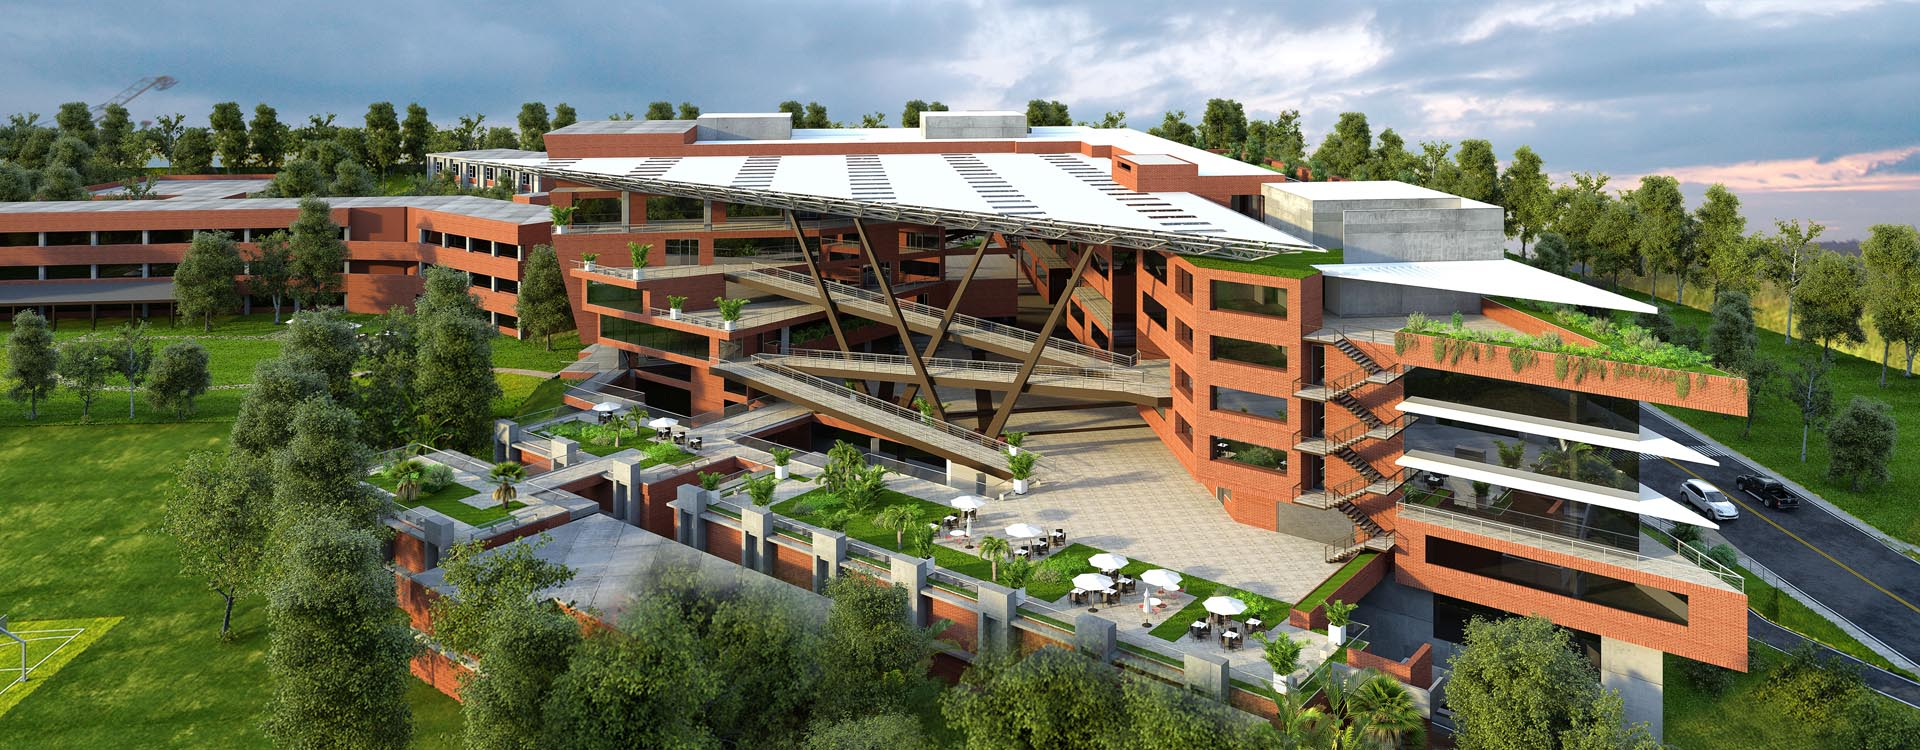
\includegraphics[height=13.25cm]{plantilla/portadacit.jpg}}
    	\makebox[\textwidth]{
    		\begin{overpic}[height=13.25cm]{\imagenportada}
     		\put(63,0){
\includegraphics[height=1.15in]{plantilla/fondologo_grande.png}}  
  			\put(64.5,2){
\includegraphics[height=0.55in]{plantilla/logoUVGblanco.eps}} 
        	\end{overpic}
    	}
    	%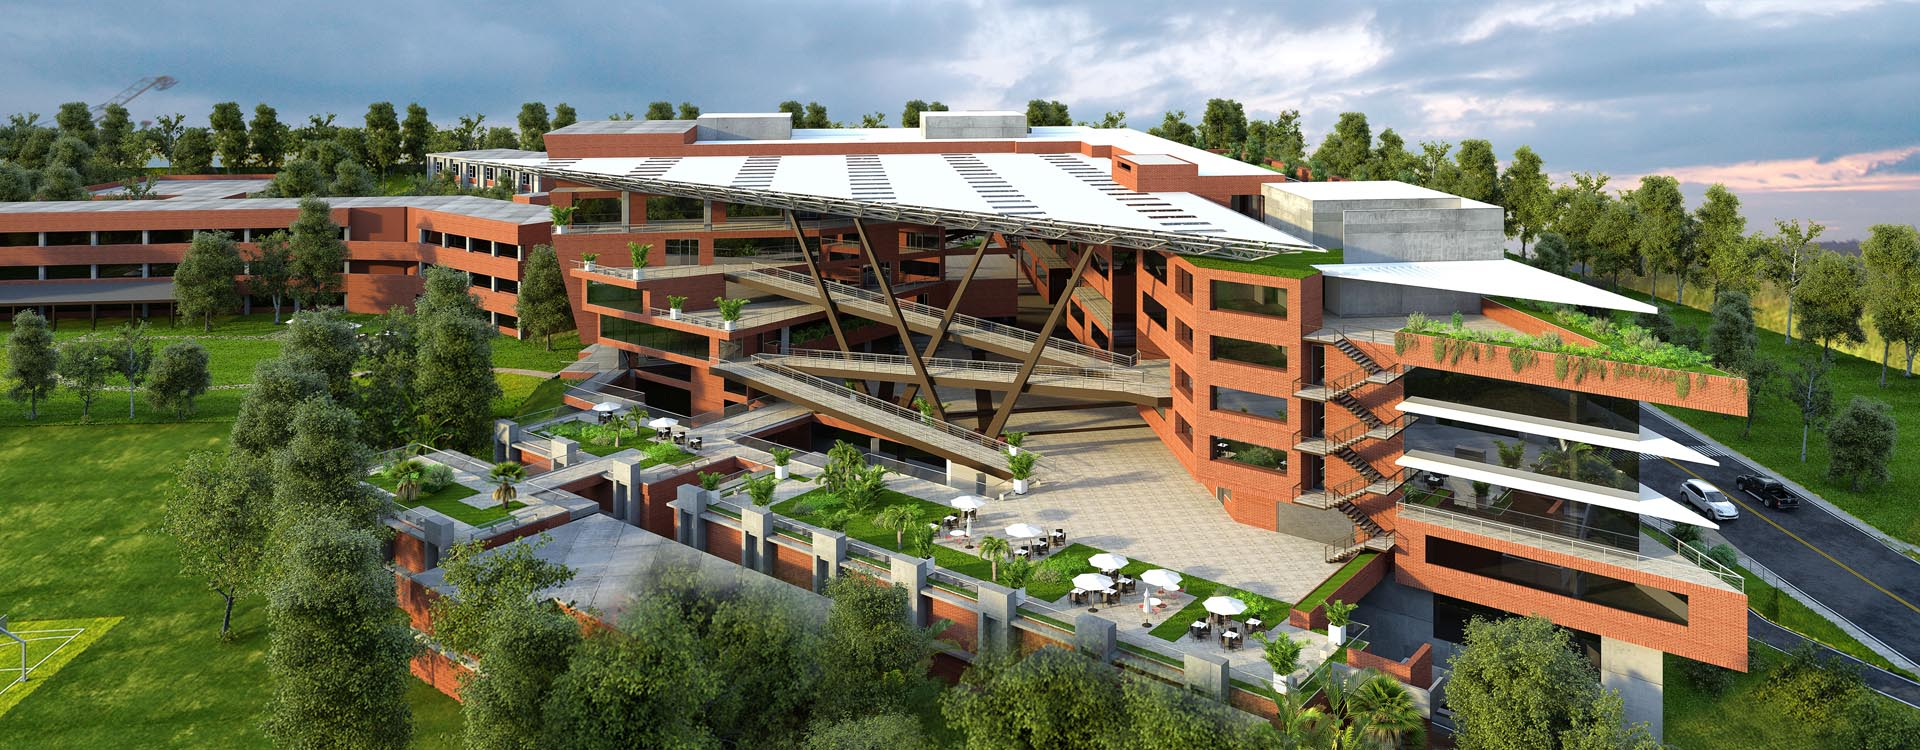
\includegraphics[height=13.25cm]{plantilla/portadacit.jpg}
	\end{figure}
	\restoregeometry
\fi

% ==============================================================================
% PRIMERAS PÁGINAS (Carátulas más hojas de guarda)
% ==============================================================================
\ifdefined\CAPcaratula
	\newpage
    \cleardoublepage\phantomsection
    % \pdfbookmark{Carátula}{toc}
	\pagecolor{white}
	\color{black}
	\setcounter{page}{1}
	\pagenumbering{roman}
	\thispagestyle{empty}
	\begin{center}
		\LARGE UNIVERSIDAD DEL VALLE DE GUATEMALA\\
		\LARGE Facultad de \uvgfacultad \\[0.75cm]
	\end{center}
	\begin{figure}[h]
		\begin{center}
		
\includegraphics[height=5.5 cm]{plantilla/escudoUVGnegro.eps}
		\vspace{0.5in}
		\end{center}
	\end{figure}
	\begin{center}
		\Large \textbf{\nohyphens{\titulotesis}} \\
		%\LARGE \textbf{\titulotesis} \\
		\vfill
		\Large \nohyphens{Trabajo de graduación presentado por \nombreestudiante \ para optar al grado académico de Licenciado en \uvgcarrera} \\
		\vfill
		\large Guatemala, \\
		\vspace{1em}
		\anoentrega
	\end{center}
    
    \ifdefined\printver	
	    \blankpage
	    \blankpage
	    
	    \newpage
	    \cleardoublepage\phantomsection
	    \pagecolor{white}
    	\color{black}
    	\setcounter{page}{1}
    	\pagenumbering{roman}
    	\thispagestyle{empty}
    	\begin{center}
    		\LARGE UNIVERSIDAD DEL VALLE DE GUATEMALA\\
    		\LARGE Facultad de \uvgfacultad \\[0.75cm]
    	\end{center}
    	\begin{figure}[h]
    		\begin{center}
    		
\includegraphics[height=5.5 cm]{plantilla/escudoUVGnegro.eps}
    		\vspace{0.5in}
    		\end{center}
    	\end{figure}
    	\begin{center}
    		\Large \textbf{\nohyphens{\titulotesis}} \\
    		%\LARGE \textbf{\titulotesis} \\
    		\vfill
    		\Large \nohyphens{Trabajo de graduación presentado por \nombreestudiante \ para optar al grado académico de Licenciado en \uvgcarrera} \\
    		\vfill
    		\large Guatemala, \\
    		\vspace{1em}
    		\anoentrega
    	\end{center}
    \fi
\fi

% ==============================================================================
% HOJA DE FIRMAS
% ==============================================================================
\ifdefined\CAPfirmas
	\newpage
	\cleardoublepage\phantomsection
	\thispagestyle{empty}
	\vspace*{0.5in}
	\large Vo.Bo.:\\[1cm]
	\begin{center}
		(f) \rule[1pt]{4 in}{1pt}\\
		\nombreasesor
	\end{center}
	\vspace{1in}

	Tribunal Examinador:\\[1cm]
	\begin{center}
		(f) \rule[1pt]{4 in}{1pt}\\
		\nombreasesor \\[1in]
		(f) \rule[1pt]{4 in}{1pt}\\
		\nombreprimerex \\[1in]
		(f) \rule[1pt]{4 in}{1pt}\\
		\nombresegundoex
	\end{center}
	\vspace{1in}

%	Fecha de aprobación: Guatemala, \rule[1pt]{0.5 in}{1pt} de \rule[1pt]{1 in}{1pt} de \anoaprobacion.
    Fecha de aprobación: Guatemala, \diaaprobacion de \mesaprobacion de \anoaprobacion.
	\normalsize
\fi

% Comentar para formato estilo libro en la numeración de páginas (NO 
% compatible con la guía UVG 2019)
\pagestyle{plain}
% ==============================================================================
% CONTENIDO DEL TRABAJO
% ==============================================================================
% PREFACIO
% ------------------------------------------------------------------------------
\ifdefined\CAPprefacio
	\newpage
	\cleardoublepage\phantomsection
    \chapter*{Prefacio}
    \ifdefined\parpordefecto
    	\defaultparformat{a-prefacio}
    \else
    	Este trabajo es el resultado de un esfuerzo continuo, y no podría haberlo logrado sin el apoyo incondicional de las personas que siempre estuvieron a mi lado a lo largo de este proceso. A mi padre, Jorge, cuyo consejo y ejemplo me han guiado en cada paso, a mi madre, Brenda, por su amor y dedicación, que me ha enseñado a enfrentar los retos con paciencia y fortaleza, y a mi hermana, Camila, por ser mi apoyo emocional constante, saber cómo distraerme cuando lo necesitaba y, sobre todo, por su incansable cariño. Cada uno de ellos ha sido esencial para mi crecimiento personal y académico, y su presencia ha sido un pilar en mi vida durante toda esta carrera.

Quiero expresar también mi sincero agradecimiento a mi asesor de tesis, el Dr. Luis Alberto Rivera Estrada, quien ha sido una fuente invaluable de conocimiento y motivación. Su disposición constante para resolver mis dudas, su paciencia para guiarme en cada etapa de este proyecto y sus palabras de aliento me han permitido superar obstáculos y continuar avanzando. Sin su apoyo, este trabajo no habría sido posible.

A mis amigos y compañeros de estos cinco años, gracias por compartir este camino lleno de retos, aprendizajes y momentos inolvidables. Su amistad ha hecho que mi experiencia universitaria haya sido mucho más enriquecedora y memorable. También a mis amigos del colegio, quienes siempre han estado presentes, ofreciéndome su apoyo y comprensión a pesar de la distancia. Su apoyo constante es un tesoro que valoro profundamente.

Finalmente, mi agradecimiento se extiende a todos los profesores que, con generosidad, han compartido su conocimiento conmigo. Gracias por extender siempre su mano y respaldarme en cada paso del camino. Su apoyo no solo ha sido crucial para la realización de este trabajo de graduación, sino también para que pudiera enfrentar cada materia con confianza y éxito.
    \fi
    \addcontentsline{toc}{chapter}{Prefacio}
\fi

% ÍNDICE GENERAL
% ------------------------------------------------------------------------------
\ifdefined\CAPindice
	\newpage
    \cleardoublepage\phantomsection
	\renewcommand{\contentsname}{Índice}
    %\phantomsection
    \pdfbookmark{\contentsname}{toc}
    %\pdfbookmark{Índice}{toc}
	\tableofcontents
\fi

% LISTADO DE FIGURAS
% ------------------------------------------------------------------------------
\ifdefined\CAPfiguras
	\newpage
    \cleardoublepage\phantomsection
	\renewcommand{\listfigurename}{Lista de figuras}
	\listoffigures
	\addcontentsline{toc}{chapter}{Lista de figuras}
\fi

% LISTADO DE CUADROS
% ------------------------------------------------------------------------------
\ifdefined\CAPcuadros
	\newpage
    \cleardoublepage\phantomsection
	\renewcommand{\listtablename}{Lista de cuadros}
	\listoftables
	\addcontentsline{toc}{chapter}{Lista de cuadros}
\fi

% RESUMEN
% ------------------------------------------------------------------------------
\ifdefined\CAPresumen
	\newpage
    \cleardoublepage\phantomsection
	\chapter*{Resumen}
	\ifdefined\parpordefecto
		\defaultparformat{b-resumen}
	\else
		Este trabajo de investigación se enfocó en la evaluación de sensores de distancia tipo láser para aplicaciones de mapeo de entornos con agentes robóticos móviles, destacando la importancia de contar con sensores precisos y confiables para la navegación autónoma. A través de un análisis comparativo entre tres sensores de distancia tipo láser: VL53L0X, LiDAR FHL-LD20, y YDLIDAR Tmini Pro, se evaluaron diversos criterios y parámetros técnicos que permitieron seleccionar al sensor LiDAR FHL-LD20 como el más adecuado para su integración en dichas aplicaciones. Adicionalmente, se desarrolló una herramienta de software diseñada par procesar, visualizar e interpretar los datos generados por el sensor seleccionado. 

La herramienta no solo facilitó la interpretación de los datos, sino que también se consolidó como un recurso clave para validar el rendimiento del sensor en diversas condiciones operativas. De forma paralela, se llevaron a cabo pruebas de calibración y caracterización del sensor en escenarios específicos. Estas pruebas permitieron definir un rango mínimo de medición efectivo, depurar mediciones nulas, y analizar las distribuciones de las mediciones de distancia y ángulo, revelando que el sensor ofrece mediciones precisas, con desviaciones menores a 5 mm en las distancias y un margen de error inferior a 3° en las mediciones angulares.

Finalmente, se evaluó la viabilidad de integrar el sensor en agentes robóticos móviles disponibles en la Universidad.  Las contribuciones de esta investigación son significativas, ya que abren el camino para futuras aplicaciones en robótica autónoma y mapeo de entornos dinámicos, aportando herramientas útiles para avanzar en la integración de sensores LiDAR en sistemas robóticos móviles.
	\fi
	\addcontentsline{toc}{chapter}{Resumen}
\fi

% ABSTRACT
% ------------------------------------------------------------------------------
\ifdefined\CAPabstract
	\newpage
    \cleardoublepage\phantomsection
	\chapter*{Abstract}
	\ifdefined\parpordefecto
		\defaultparformat{c-abstract}
	\else
		This research focused on the evaluation of laser distance sensors for environment mapping applications with mobile robotic agents, emphasizing the importance of precise and reliable sensors for autonomous navigation. Through a comparative analysis of three laser distance sensors: VL53L0X, LiDAR FHL-LD20, and YDLIDAR Tmini Pro, various technical criteria and parameters were assessed, leading to the selection of the LiDAR FHL-LD20 as the most suitable for integration in such applications. Additionally, a software tool was developed to process, visualize, and interpret the data generated by the selected sensor.

The tool not only facilitated data interpretation but also became a key resource for validating the sensor’s performance under different operational conditions. Simultaneously, calibration and characterization tests were carried out in specific scenarios. These tests helped define the sensor's minimum effective measurement range, refine data by filtering out null measurements, and analyze the distributions of distance and angle readings, revealing that the sensor provides precise measurements with deviations of less than 5 mm in distances and a margin of error below 3° in angular measurements.

Finally, the feasibility of integrating the sensor into available mobile robotic agents at the University was assessed. The contributions of this research are significant, as they pave the way for future applications in autonomous robotics and dynamic environment mapping, providing valuable tools to advance the integration of LiDAR sensors into mobile robotic systems.
	\fi
	\addcontentsline{toc}{chapter}{Abstract}
\fi

% INTRODUCCIÓN
% ------------------------------------------------------------------------------
\ifdefined\CAPintroduccion
	\newpage
	\cleardoublepage
	\pagenumbering{arabic}
	\setcounter{page}{1}
	\chapter{Introducción}
	\ifdefined\parpordefecto
		\defaultparformat{d-introduccion}
	\else
		El objetivo principal de este trabajo fue evaluar tecnologías y opciones de sensores de distancia que puedan usarse para mapeo de entornos. Para ello, se llevó a cabo un análisis de las opciones disponibles en el mercado, considerando distintos criterios, y se seleccionó la mejor opción que se consideraba adecuada para su futura implementación con agentes robóticos móviles. Asimismo, se desarrolló una herramienta de software que permitió la comunicación con el sensor seleccionado, permitiendo adquirir, interpretar y visualizar los datos capturados de manera intuitiva y eficiente. 

Además, con esta herramienta, se caracterizó y calibró el LiDAR FHL-LD20, con el objetivo de optimizar su rendimiento y validar su precisión. Se llevaron a cabo pruebas en distintos entornos controlados para evaluar su funcionamiento y la fidelidad de sus mediciones bajo diferentes condiciones. Durante este proceso, se establecieron criterios de comparación y evaluación para analizar el desempeño del mismo. De esta manera, se identificaron posibles limitaciones y áreas de mejora, con el fin de optimizar su uso y garantizar fiabilidad de los datos obtenidos para su futura implementación en aplicaciones de mapeo y navegación en el ecosistema Robotat de la Universidad del Valle de Guatemala.
	\fi
\fi

% ANTECEDENTES
% ------------------------------------------------------------------------------
\ifdefined\CAPantecedentes
	\newpage
	\chapter{Antecedentes}
	\ifdefined\parpordefecto
    	\defaultparformat{e-antecedentes}
    \else
    	En el campo de la robótica móvil, la navegación autónoma desempeña una tarea fundamental para que los sistemas robóticos se desplacen de manera segura y eficiente en entornos dinámicos y desconocidos. Este proceso implica la percepción del entorno mediante sensores, la planificación y ejecución de trayectorias y la toma de decisiones en tiempo real, sin la necesidad de intervención humana directa. Por lo tanto, la exitosa integración de este proceso resulta en una mayor capacidad de adaptación y desempeño de los robots móviles con su entorno, promoviendo la autonomía e independencia de estos sistemas.

\section{Generación de trayectorias y mapeo de entornos}
En \cite{li_map_2023} se describió un método de construcción para mapeo de entornos basado en un mapa de cuadrícula de probabilidad de colisión y la mejora de un algoritmo A*. Se utilizaron técnicas de probabilidad de colisión que consideraron tanto el tamaño del robot como la posición relativa de este y los obstáculos presentes en la cuadrícula para construir un mapa del entorno. El método permitió encontrar rutas seguras y eficientes al integrar información de probabilidad de colisión en el proceso de construcción de mapas y planificación de rutas desde el nodo de inicio hasta el nodo objetivo. El mapa generado ofrece una cuadrícula en escala de grises indicando la probabilidad de colisión según la cercanía de los obstáculos; cuanto más oscuro el color, más peligroso y cercano se encuentra el obstáculo. En cambio, la cuadrícula blanca representa la zona libre y menos propensa a la colisión.

\begin{figure}[H]
	\centering
	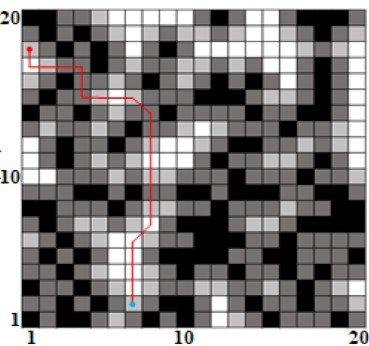
\includegraphics[width=0.45\textwidth]{mapa_colisiones.jpg}
	\caption{Mapa generado a partir de cuadrícula de probabilidad de colisión con ruta óptima \cite{li_map_2023}.}
	\label{fig2_1}
\end{figure}

Además, considera la función de costo del algoritmo A*, minimizando el tiempo de búsqueda de nodos peligrosos en entornos complejos, generando un mapa más completo y reduciendo el tiempo de búsqueda y número de giros en las rutas propuestas. Los resultados de las simulaciones realizadas en Matlab demuestran mejoras en la seguridad ante colisiones y eficiencia de localización de objetos en entornos complejos sobre algoritmos tradicionales. Sin embargo, los autores identifican ciertas limitaciones ante obstáculos dinámicos al momento de mapear el entorno.\\

En \cite{li_quadruped_2022} se desarrolló e implementó un algoritmo para el mapeo bidimensional en robots cuadrúpedos utilizando estimaciones de mínimos cuadrados. El algoritmo generado tuvo como finalidad planificar y producir trayectorias de seguimiento que permitieron la evasión de obstáculos en entornos cambiantes. Esto se logró por medio de un radar láser 3D y un sistema de posicionamiento de banda ultraancha (UWB) los cuales proporcionaban datos espaciales y direccionales del entorno en tiempo real. Dicha información fue transformada en un mapa de rejilla 2D donde se estableció la ubicación actual del cuadrúpedo, la presencia de obstáculos y los espacios libres de movimiento. El artículo presentó resultados experimentales que demostraron la precisión del algoritmo en la construcción del entorno y la autonomía del cuadrúpedo al ajustar sus movimientos y trayectorias en tiempo real según diferentes situaciones. Además, se destacó la futura implementación de algoritmos de trayectorias globales y locales para mejorar la reconstrucción del entorno y la estabilidad del sistema de planificación de rutas y navegación espacial.

\section{\textit{Ant Colony Optimization} (ACO)}

En \cite{dai_mobile_2019} se compararon algoritmos basados en ACO para abordar la problemática de planificación de rutas para robots móviles en entornos complejos. En el artículo se analizaron diferentes parámetros para determinar tanto la convergencia de las trayectorias como la optimización y suavidad de las rutas en diferentes entornos de simulación para cada uno de los algoritmos propuestos. Además, se destacó la implementación de mecanismos de reacción y supresión de curvas para mejorar el rendimiento y adaptabilidad de estos, resultando en un algoritmo que superó en eficiencia y convergencia las versiones tradicionales de ACO. Los resultados de simulación en MATLAB demostraron que el algoritmo mejorado garantiza que los robots puedan encontrar una trayectoria satisfactoria incluso en situaciones desafiantes.


\begin{figure}[H]
	\centering
	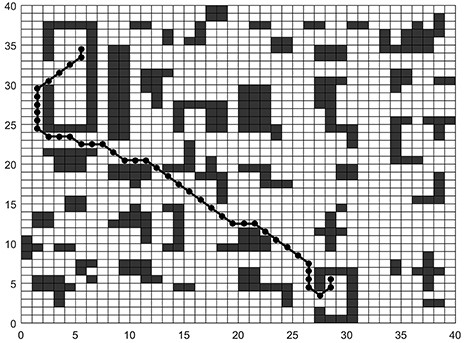
\includegraphics[width=0.6\textwidth]{ruta_algoritmo_mod.jpg}
	\caption{Ruta generada a partir del algoritmo ACO mejorado \cite{dai_mobile_2019}.}
	\label{fig2_2}
\end{figure}

\section{\textit{Particle Swarm Optimization} (PSO)}
En \cite{han_mobile_2019} se presentó la implementación de PSO para la planificación de rutas de robots móviles en coordenadas polares. Se empleó el algoritmo de optimización por enjambre de partículas como un proceso de búsqueda donde cada agente se movió a través de un espacio bidimensional buscando la mejor ruta desde el punto de inicio hasta el punto objetivo. Durante la ejecución del algoritmo, los agentes se movieron a través del espacio de búsqueda, ajustando su posición y velocidad en función de la información obtenida de su propio desempeño pasado y de la mejor solución global encontrada por otros agentes en el enjambre. Este proceso de búsqueda colectiva permitió que los agentes exploraran el espacio y convergieran hacia soluciones óptimas. Los resultados de simulación demostraron que el algoritmo PSO eliminó puntos de ruta redundantes, optimizando la eficiencia de trayectorias planificadas. Sin embargo, los autores identificaron ciertas limitaciones de escalabilidad en entornos con obstáculos dinámicos. 

\section{Implementación de algoritmos de inteligencia de enjambre en UVG}
En el trabajo de investigación \cite{pena_echeverria_algoritmo_2019} se desarrolló e implementó un algoritmo de control para sistemas de robots multi-agente orientado a misiones de búsqueda, basado en métodos teóricos de grafos y control moderno. Se destacó que la integración de una sola función racional que combina el control de formación y colisiones permitía que los agentes alcanzaran formaciones con un mínimo error cuadrático medio al utilizar grafos totalmente rígidos. Además, los resultados de la simulación en el entorno de Webots demostraron que los agentes lograron alcanzar la meta en el 80\% de los escenarios considerados, con un 11\% de éxito en control de formación. Esto indicó que el algoritmo propuesto fue efectivo en la coordinación de los agentes, más no fue eficiente en la cantidad de formaciones finales exitosas.

\begin{figure}[H]
	\centering
	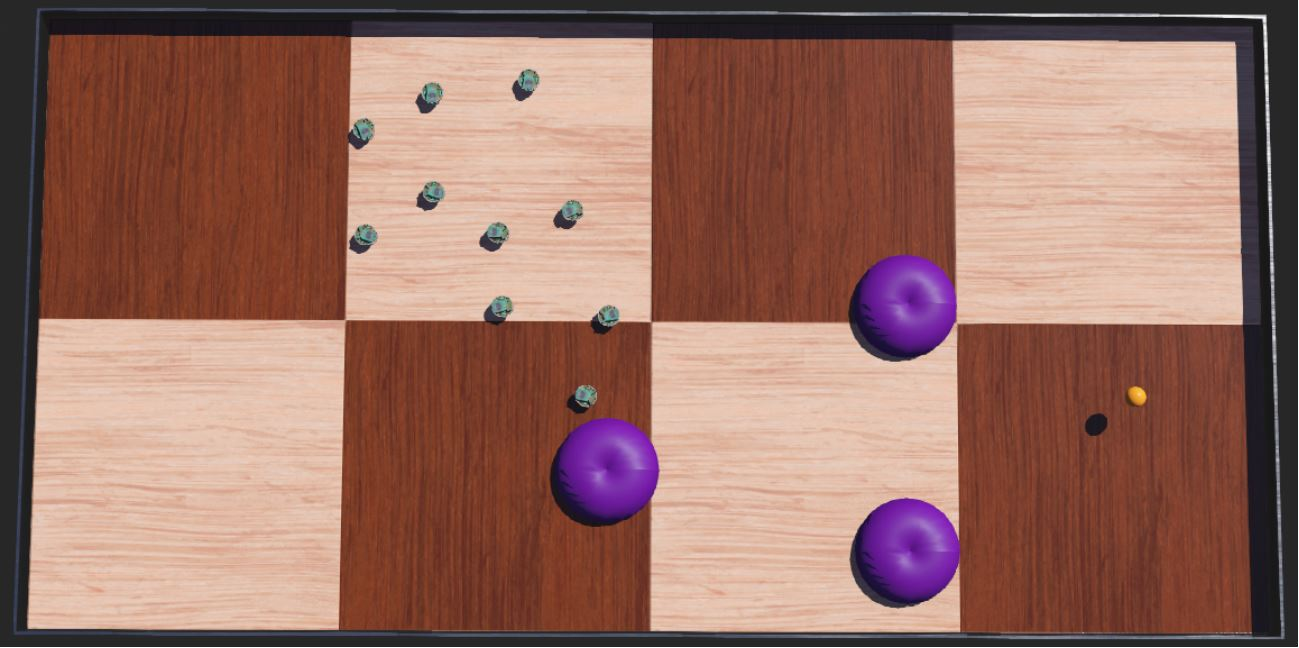
\includegraphics[width=0.75\textwidth]{desplazamiento.jpg}
	\caption{Desplazamiento del grupo de robots hacia la meta  \cite{pena_echeverria_algoritmo_2019}.}
	\label{fig2_3}
\end{figure}

\begin{figure}[H]
	\centering
	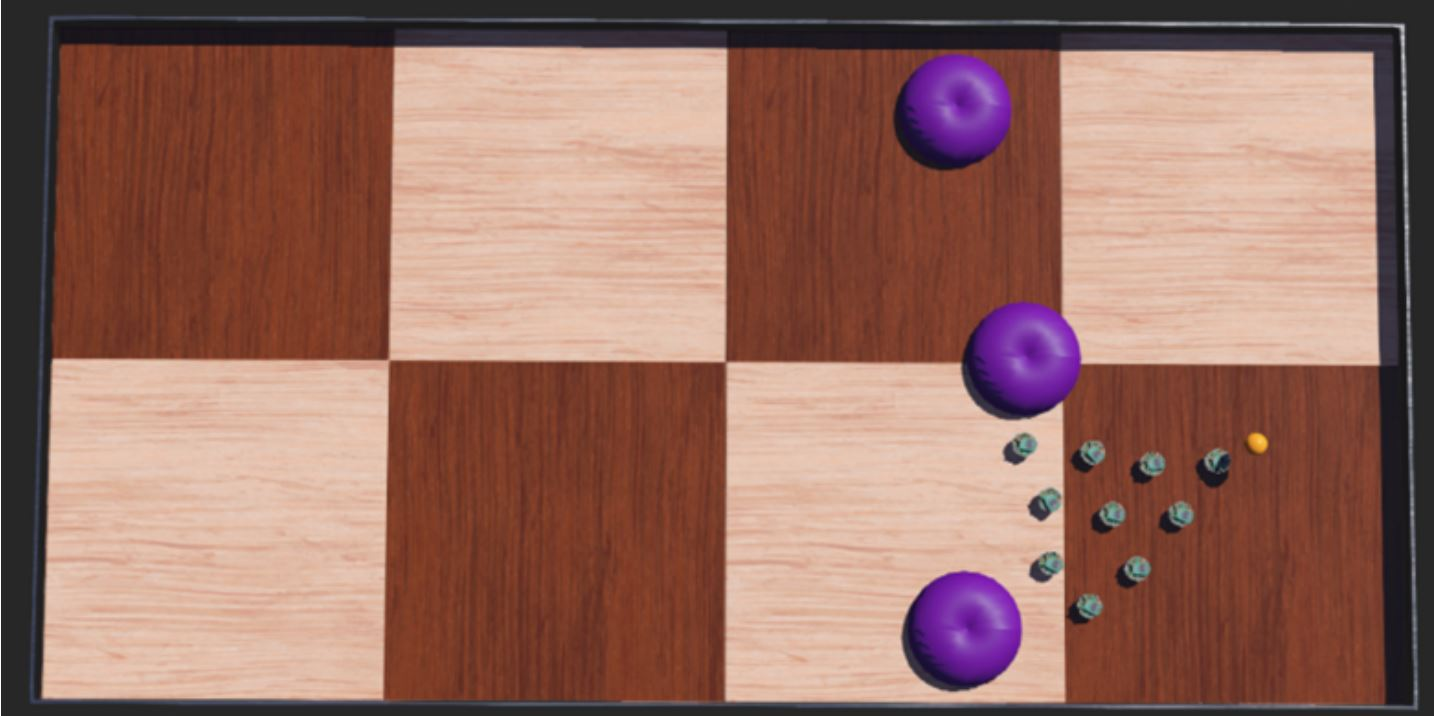
\includegraphics[width=0.75\textwidth]{formacion.jpg}
	\caption{Formación triangular del grupo de robots en la meta \cite{pena_echeverria_algoritmo_2019}.}
	\label{fig2_4}
\end{figure}

En \cite{santizo_olivet_aprendizaje_2021} se desarrolló un algoritmo que determinaba los parámetros más adecuados para mejorar y potenciar el desempeño del algoritmo PSO estándar. Mediante el uso de redes neuronales recurrentes, la herramienta nombrada Deep PSO Tuner, permitió la selección dinámica y automática de los hiper-parámetros que debería de emplear el algoritmo, mejorando la precisión y tiempo de convergencia del mismo. Los resultados de las simulaciones realizadas demostraron que la red nueronal BiLSTM fue la más efectiva, logrando superar obstáculos locales y permitiendo una mayor precisión y rendimiento del algoritmo en diferente situaciones. No obstante, se mencionaron ciertas limitaciones respecto a la escalabilidad del método y la baja reacción del algoritmo en situaciones con obstáculos dinámicos.

En el trabajo de investigación \cite{baldizon_garcia_aplicaciones_2022} se propusieron dos algoritmos basados en ACO para resolver problemas de exploración de terrenos, planificación de trayectorias y evasión de obstáculos. Los algoritmos fueron implementados en Matlab y se realizaron validaciones a nivel de simulación en el entorno de Webots de Cybertbotics. Los resultados de este trabajo evidenciaron que las trayectorias generadas por los algoritmos condujeron a que los agentes móviles evadieran exitosamente los obstáculos presentes en el entorno. Asimismo, las modificaciones realizadas al algoritmo, resultaron en mejoras significativas en la autonomía y rendimiento de los agentes y en la fidelidad de las replicas de los entornos explorados.
\begin{figure}[H]
	\centering
	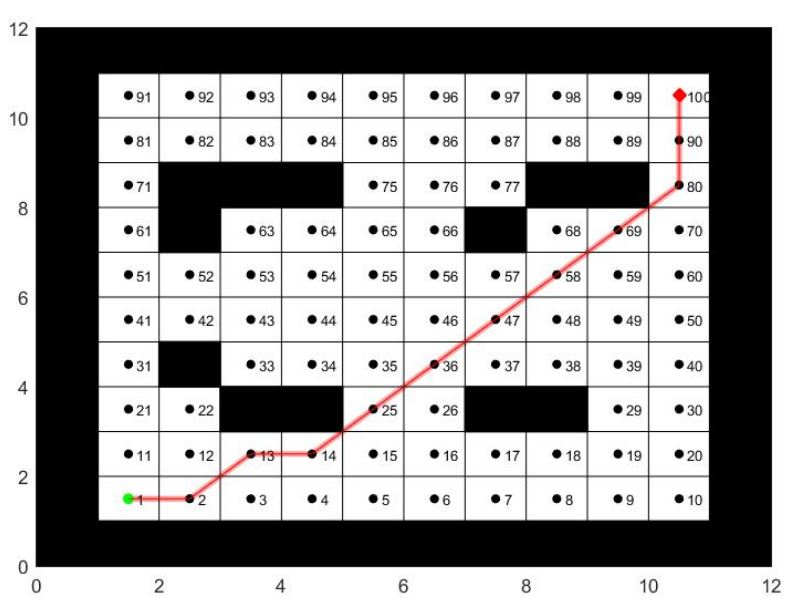
\includegraphics[width=0.5\textwidth]{mapa.jpg}
	\caption{Mapa y trayectoria generada para la validación en Webots \cite{baldizon_garcia_aplicaciones_2022}.}
	\label{fig2_5}
\end{figure}

\begin{figure}[H]
	\begin{subfigure}{0.5\textwidth}
		\centering
		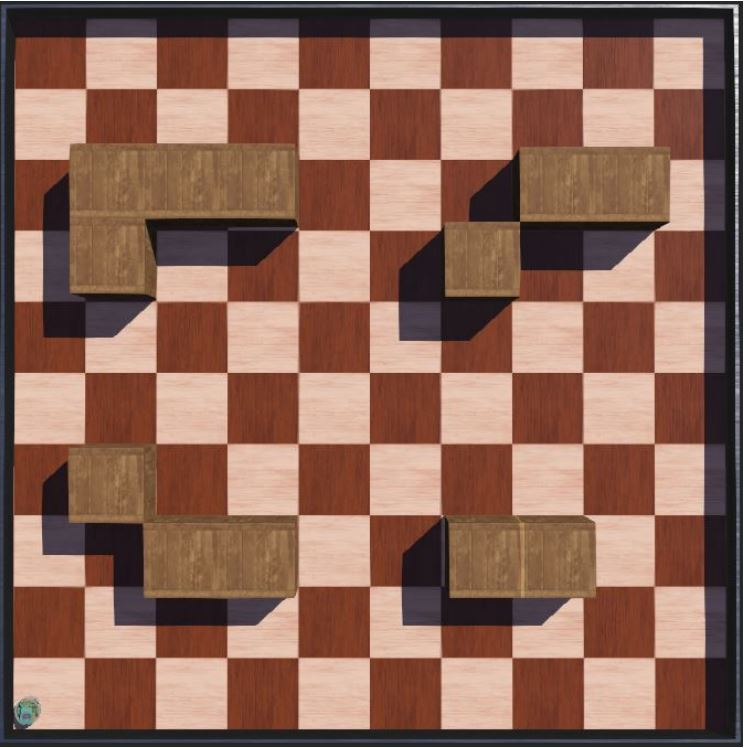
\includegraphics[width=0.9\linewidth]{pos_ini.jpg}
		\caption{Posición inicial.}
	\end{subfigure}
	\begin{subfigure}{0.5\textwidth}
		\centering
		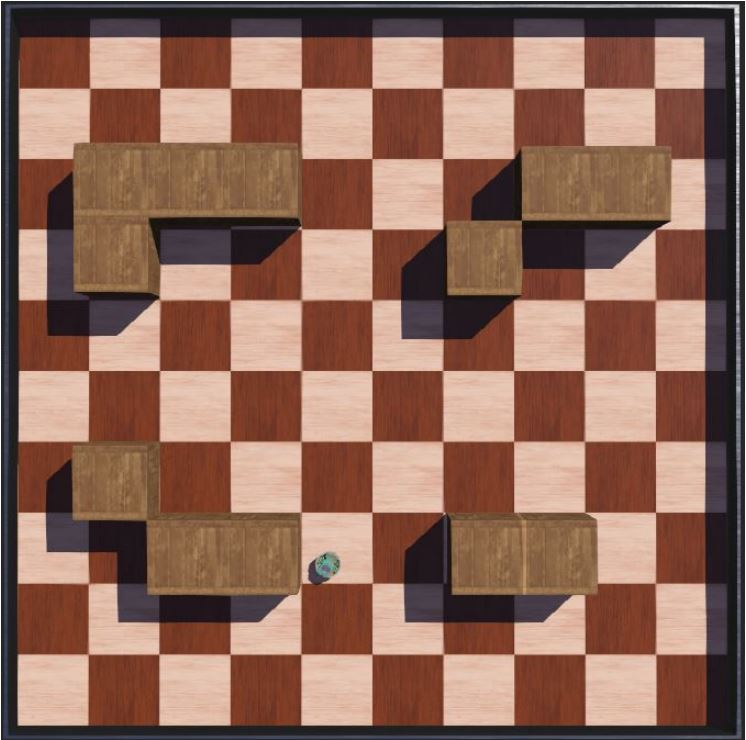
\includegraphics[width=0.9\linewidth]{pos_int1.jpg}
		\caption{Posición intermedia.}
	\end{subfigure}
	\begin{subfigure}{0.5\textwidth}
		\centering
		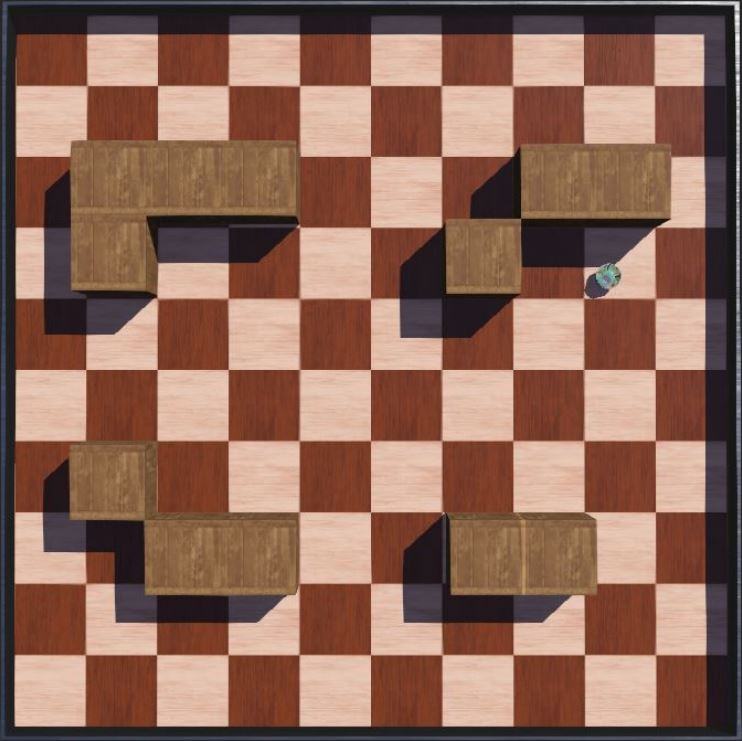
\includegraphics[width=0.9\linewidth]{pos_int2.jpg}
		\caption{Posición intermedia.}
	\end{subfigure}
	\begin{subfigure}{0.5\textwidth}
		\centering
		
\includegraphics[width=0.9\linewidth]{pos_fin.jpg}
		\caption{Posición final.}
	\end{subfigure}
	\caption{Secuencia de movimientos del agente móvil para la evasión de obstáculos en Webots \cite{baldizon_garcia_aplicaciones_2022}.}
	\label{fig2_6}
\end{figure}


En \cite{godoy_lucero_desarrollo_2023} se desarrollaron y evaluaron algoritmos para el mapeo de entornos y generación de trayectorias utilizando sistemas robóticos multi-agente. Se enfocó en la implementación simulada de la combinación de tres algoritmos relacionados con la navegación autónoma en robots con tracción diferencial. Estos algoritmos abarcaron la exploración de entornos, el mapeo bidimensional de los mismos y la generación óptima de trayectorias. Para llevar a cabo la validación, se desarrollaron y simularon en Webots distintos escenarios de trabajo que incluían pasillos,  espacios abiertos y obstáculos tridimensionales. Estos entornos fueron reconstruidos,  de manera individual y colectiva, por agentes robóticos móviles con sensores de distancia integrados: cinco sensores frontales separados por un ángulo de 45 grados entre sí y un único sensor colocado en la parte trasera del vehículo.

\begin{figure}[H]
	\centering
	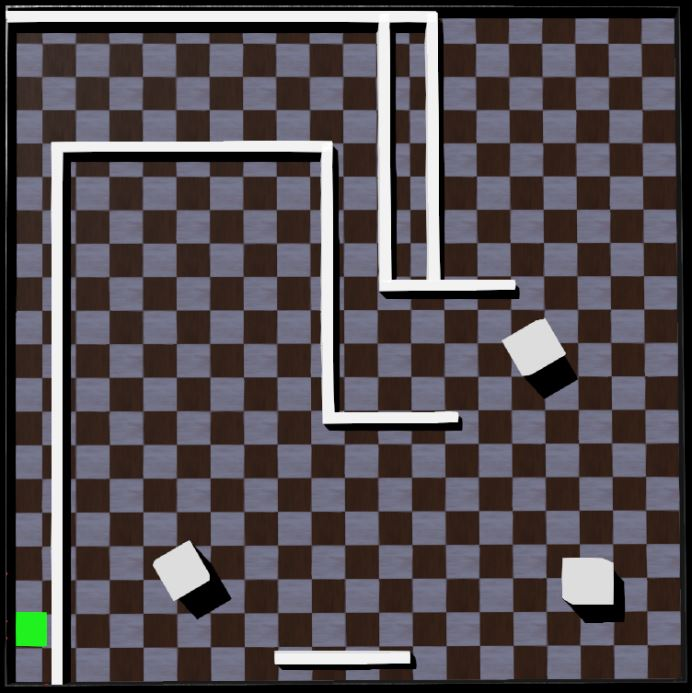
\includegraphics[width=0.6\textwidth]{escenario.jpg}
	\caption{Escenario simulado en Webots \cite{godoy_lucero_desarrollo_2023}.}
	\label{fig2_7}
\end{figure}

\begin{figure}[H]
	\centering
	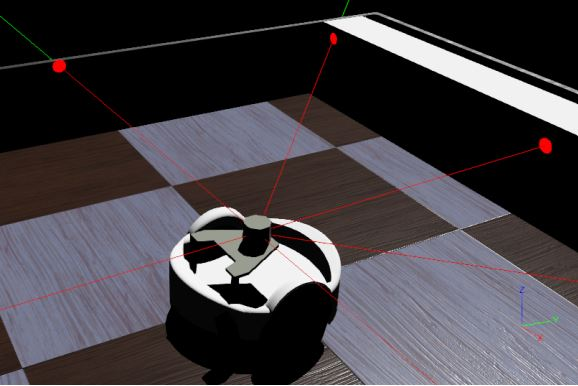
\includegraphics[width=0.5\textwidth]{exploracion.jpg}
	\caption{Puntos de visibilidad de los sensores integrados en el agente robótico móvil en Webots. \cite{godoy_lucero_desarrollo_2023}.}
	\label{fig2_8}
\end{figure}


En las simulaciones computarizadas, se observó que la integración de sensores a distancia tipo láser en lugar de los tipo sonar en los agentes resultaba más precisa y eficaz en la detección de obstáculos, asegurando trayectorias de exploración confiables y no redundantes. Además, se destacó que la disposición e interacción entre estos sensores influía en la capacidad del sistema para obtener una representación precisa del entorno. Se decidió combinar los datos provenientes de todos los sensores delanteros para compensar las limitaciones individuales de cada sensor, obteniendo una buena estimación y reconstrucción del entorno. La precisión en la distribución y disposición de los obstáculos en las estimaciones del espacio de trabajo permitieron el desarrollo y validación del algoritmo de planificación de trayectorias en mapas previamente explorados. Basándose en las validaciones simuladas de los algoritmos desarrollados, el autor recomienda dos sensores de distancia comerciales para la implementación física de estos algoritmos en futuros estudios. No obstante, se mencionaron ciertas limitaciones respecto a la representación exacta del entorno debido a la falta de información en ciertas áreas por el tiempo de simulación y colisiones recurrentes por obstáculos imprevistos, como la esquina de un obstáculo. 

\begin{figure}[H]
	\centering
	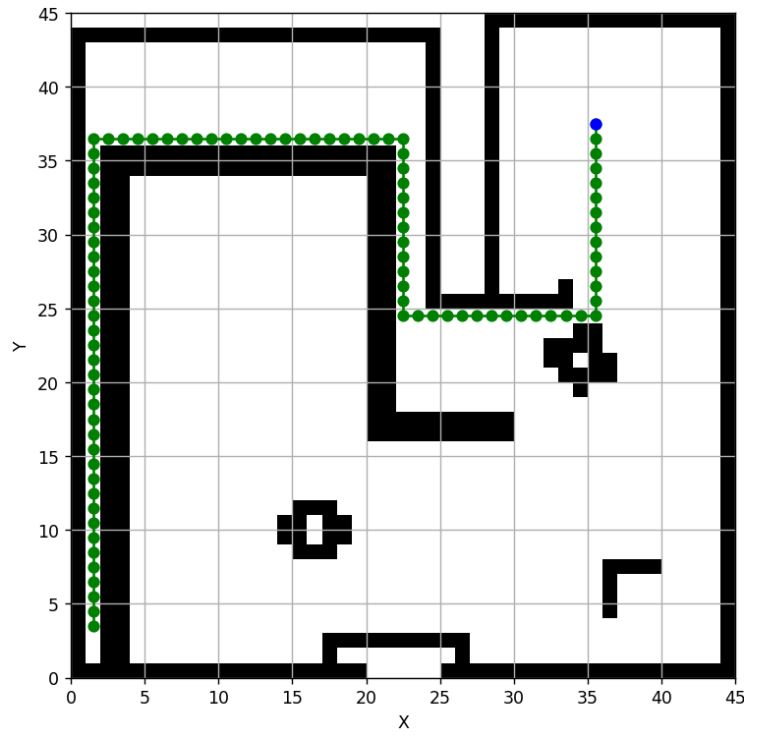
\includegraphics[width=0.55\textwidth]{mapeo.jpg}
	\caption{Espacio de trabajo estimado en exploración de 10 minutos, con planificación de trayectoria hacia su posición inicial de simulación  \cite{godoy_lucero_desarrollo_2023}.}
	\label{fig2_9}
\end{figure}

\section{Robotat}
En las instalaciones de la Universidad del Valle de Guatemala, se encuentra un laboratorio especializado en la experimentación robótica denominado Robotat. Inspirado en el Robotarium del Instituto de Tecnología de Georgia \cite{maderer_robotarium_nodate}, Estados Unidos, este espacio cuenta con una plataforma de acero blanca de 4.8 × 3.8 m, rodeada por el sistema de captura de movimiento OptiTrack. Dicho sistema está conformado por seis cámaras de alta precisión y baja latencia, diseñadas para capturar movimiento en tiempo real. Además, el laboratorio dispone de una red WiFi local que permite la comunicación entre los robots. Este entorno ha creado un ecosistema integral de aprendizaje, investigación y desarrollo práctico en el campo de la robótica \cite{barrera_robotat_nodate}.

En los sistemas de captura de movimiento, el uso eficiente de las cámaras es fundamental para procesar de manera óptima las imágenes obtenidas. En el caso del Robotat, el sistema OptiTrack utiliza marcadores reflectivos de plástico conocidos como marcadores pasivos para calcular con precisión la localización tridimensional de los objetos \cite{perafan_camilo_2022}. Estos marcadores reflejan la luz infrarroja emitida por las cámaras, lo que permite su detección dentro de la plataforma. Además, pueden adherirse a diversos objetos para rastrear su posición dentro del espacio 3D que abarca la plataforma, facilitando un seguimiento detallado y preciso de los movimientos.

\begin{figure}[H]
	\centering
	\includegraphics[width=0.75\textwidth]{robotat.jpg}
	\caption{Robotat, laboratorio especializado en experimentación robótica.}
	\label{robotat}
\end{figure}
    \fi  
\fi

% JUSTIFICACIÓN
% ------------------------------------------------------------------------------
\ifdefined\CAPjustificacion
	\newpage
	\chapter{Justificación}
	\ifdefined\parpordefecto
		\defaultparformat{f-justificacion}
	\else
		En entornos desconocidos, los robots móviles deben ser capaces de desplazarse de un punto a otro de manera eficiente y segura tomando en cuenta los obstáculos y elementos de interés dentro del área de operación. En los trabajos de fases anteriores se han desarrollado e implementado, a nivel de simulación, algoritmos de exploración para el mapeo de entornos utilizando modelos virtuales de robots con tracción diferencial. El uso de estos algoritmos junto con las estimaciones del entorno han permitido que se evalúe el rendimiento de algoritmos para la planificación de trayectorias en espacios donde se desee llevar a cabo una navegación autónoma. Sin embargo, todos los avances que se han realizado han sido a nivel de simulación en software como Matlab y Webots, por lo que no se ha tenido una validación física de los algoritmos en robots móviles funcionales. 

Por esta razón, el enfoque principal de este trabajo es abordar, evaluar y seleccionar opciones de sensores de distancia que permitan la futura validación física de los algoritmos de exploración y mapeo de entornos en agentes robóticos móviles. Se busca verificar que, con los datos capturados del sensor, las estimaciones del espacio de trabajo sean consistentes con las mediciones del espacio en sí. Además, se propone buscar posibles formas de implementación para integrar los sensores de distancia a los robots diferenciales Pololu 3Pi+, lo cual dotaría a los agentes con capacidades adicionales. Esto establecería un precedente con buena base para futuras implementaciones en esta línea de investigación, como lo puede ser el mapeo de entornos físicos dinámicos.

El mapeo de entornos utilizando robots móviles resulta fundamental en una amplia gama de aplicaciones, desde la logística en el transporte de suministros en ambientes comerciales hasta la exploración de terrenos desconocidos en operaciones de búsqueda y rescate. La capacidad de generar mapas detallados que representen con precisión obstáculos y elementos relevantes, no solo mejora la comprensión del entorno sino que también establece una base sólida para la toma de decisiones y planificación de acciones en situaciones críticas, como desastres naturales. Estos mapas permiten identificar rutas seguras y evaluar riesgos en las operaciones, lo que mitiga los impactos negativos en situaciones de emergencia para los humanos.
	\fi
\fi

% OBJETIVOS
% ------------------------------------------------------------------------------
\ifdefined\CAPobjetivos
	\newpage
	\chapter{Objetivos}
	\ifdefined\parpordefecto
		\defaultparformat{g-objetivos}
	\else
		\section{Objetivo general}
Evaluar sensores de distancia tipo láser para aplicaciones de mapeo de entornos con agentes robóticos móviles.

\section{Objetivos específicos}
\begin{itemize}
	\item  Seleccionar un sensor de distancia tipo láser que sea factible para investigaciones con robots móviles en el ecosistema Robotat.
	\item Desarrollar una herramienta de software que permita la obtención e interpretación de los datos provenientes del sensor seleccionado.
	\item Realizar una caracterización detallada del sensor empleado. 
	\item Desarrollar métodos de prueba y definir criterios de evaluación para la calibración del sensor.
	\item Evaluar la futura integración del sensor en agentes robóticos móviles disponibles en la Universidad.
\end{itemize}
	\fi
\fi

% ALCANCE
% ------------------------------------------------------------------------------
\ifdefined\CAPalcance
	\newpage
	\chapter{Alcance}
	\ifdefined\parpordefecto
    	\defaultparformat{h-alcance}
    \else
    	El alcance de este proyecto incluyó el desarrollo una aplicación capaz de capturar, procesar y visualizar las mediciones proporcionadas por el sensor LiDAR FHL-LD20, así como la realización de pruebas físicas para su caracterización y calibración. Estas tareas se llevaron a cabo utilizando herramientas de software como Python y MATLAB. Además, se generaron reconstrucciones precisas basadas en los datos obtenidos del sensor, las cuales permitieron evaluar su rendimiento y ajustar sus parámetros de medición.
	
De cara a proyectos futuros o trabajos relacionados con el mapeo de entornos y la navegación autónoma, la información recolectada por el sensor podrá integrarse a los algoritmos de navegación de robots móviles. Esto abrirá la posibilidad de implementar funcionalidades avanzadas, como la planificación de trayectorias para navegación punto a punto, optimizando así el desempeño de robots en aplicaciones como la exploración, la detección de obstáculos y el control autónomo en diversos entornos.
    \fi 
\fi

% MARCO TEÓRICO
% ------------------------------------------------------------------------------
\ifdefined\CAPmarcoteorico
	\newpage
	\chapter{Marco teórico}
	\ifdefined\parpordefecto
		\defaultparformat{i-marco_teorico}
	\else
		\section{Interacción de un robot móvil con su entorno}
El entorno o mundo en el que opera un robot se define por su estado, que engloba las condiciones y características tanto del robot mismo como del entorno circundante. Sin embargo, en la práctica, especificar un estado completo es prácticamente imposible para cualquier sistema robótico realista. Esto se debe a que un estado completo abarcaría no solo todos los aspectos del entorno que podrían tener un impacto en el futuro, sino también las propias características y estados internos del propio robot. Por lo tanto, en las implementaciones prácticas se selecciona un pequeño subconjunto de todas las variables de estado para formar un estado representativo y manejable. Esta selección incluye variables como \cite{thrun_probabilistic_2005}: 
\begin{itemize}
	\item La pose del robot: Comprende su ubicación y orientación con respecto a un marco de coordenadas global. Para un robot móvil en un entorno plano, la pose suele estar constituida por sus dos coordenadas de ubicación en el plano y su orientación de giro (\textit{yaw}) \cite{thrun_probabilistic_2005}.
	\item La velocidad del robot: En un entorno plano, las velocidades críticas para un robot móvil de dos ruedas son la velocidad lineal y la angular. La velocidad lineal indica cuán rápido avanza el robot en línea recta a lo largo de su trayectoria, mientras que la velocidad angular determina la rapidez con la que el robot gira alrededor de su centro de giro. Esta última se regula ajustando las velocidades angulares de las ruedas izquierda y derecha \cite{thrun_probabilistic_2005}.
	\item La ubicación y características de los objetos circundantes  en el entorno: Este aspecto abarca características como la apariencia visual de objetos, su forma, tamaño, disposición espacial y cualquier otra propiedad relevante para la interacción del robot con su entorno. Estas variables son cruciales para interpretar y comprender la situación del robot en distintos escenarios \cite{thrun_probabilistic_2005}.  
\end{itemize}

Además de lo anterior, se distinguen dos tipos fundamentales de interacciones entre un robot y su entorno: la influencia del robot en el estado mediante acciones de control de sus actuadores y la recopilación de información del estado a través de los sensores del propio robot. Las acciones de control, como el movimiento del robot y la manipulación de objetos, provocan cambios instantáneos en el estado del entorno lo que demanda una continua adaptación y respuesta por parte del sistema robótico para actualizar las condiciones del mismo. Por otro lado, se utilizan los sensores para capturar información sobre el estado del entorno. Sin embargo, es común que las mediciones de los sensores tengan cierto retraso, por lo que proporcionan una percepción del estado en momentos relativamente anteriores \cite{thrun_probabilistic_2005}. 

\begin{figure}[H]
	\centering
	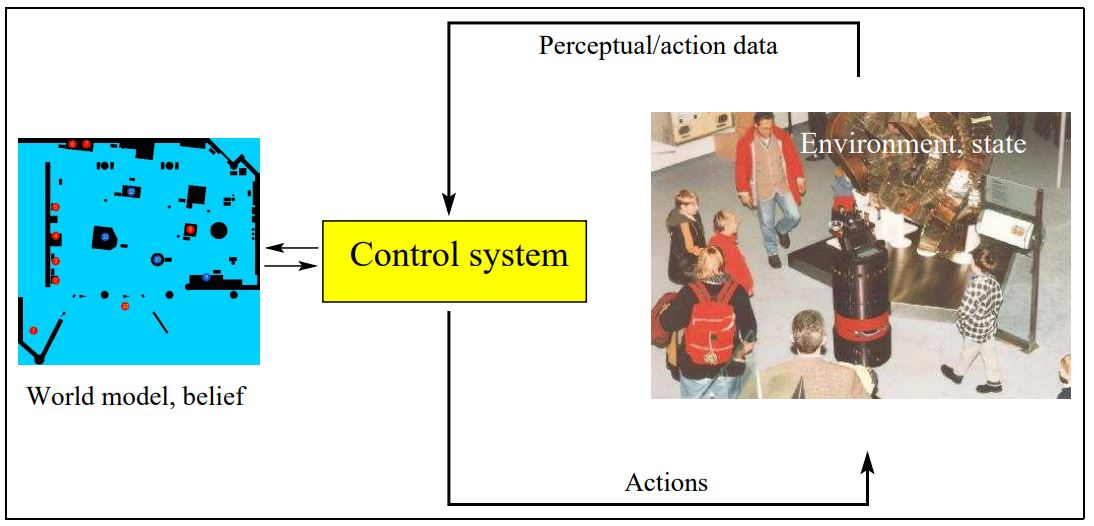
\includegraphics[width=0.7\textwidth]{inter_ent.jpg}
	\caption{Interacción de un robot con su entorno \cite{thrun_probabilistic_2005}.}
	\label{fig:interaccion_ent}
\end{figure}

\section{Modelos probabilístico de movimiento para robots móviles en entornos planos}
Los modelos probabilísticos de movimiento son empleados en robótica móvil para estimar la posición futura de un robot en función de su movimiento y de las incertidumbres asociadas que puedan influir en su trayectoria como la imprecisión de los sensores, la presencia de fuerzas externas, el ruido, entre otros. Un enfoque comúnmente utilizado es el modelo de movimiento de velocidad, el cual se basa en la relación entre las velocidades lineales y angulares del robot y su ubicación actual en el espacio para predecir su posición futura. Esta metodología en particular ofrece ventajas significativas como su facilidad de implementación y simplicidad para predecir, de manera directa, el movimiento futuro del robot en entornos simples y controlados \cite{thrun_probabilistic_2005}.

Por otro lado, se pueden emplear las mediciones de odometría como base para calcular el movimiento del robot a lo largo del tiempo. La odometría es una técnica utilizada en navegación para estimar la posición y desplazamiento de un vehículo móvil por medio de de la medición de las distancias recorridas por sus ruedas o sistemas de locomoción. Este enfoque, conocido como modelo de odometría, integra la información de los encoders en las ruedas para medir la rotación de las mismas y calcular la distancia recorrida. Estas mediciones combinadas con otros datos de orientación son empleados para estimar la posición actual del robot. Sin embargo, este método sufre de errores acumulativos a medida que el robot se desplaza debido a pequeñas desviaciones en la rotación de las ruedas \cite{thrun_probabilistic_2005}. 

Alternativamente, existe un modelo más complejo, que considera la cinemática del robot con la geometría del mismo. El modelo de movimiento cinemático considera la velocidad lineal y angular del robot, junto con la forma y tamaño del mismo para predecir con precisión el desplazamiento y la orientación futura del robot. Este enfoque destaca por su capacidad para capturar el comportamiento del robot en el espacio, ofreciendo una representación más completa del movimiento. Además, su consideración en la geometría proporciona un análisis más profundo en cómo el diseño del robot influye en su movimiento \cite{fahimi_autonomous_2009}.

\section{Robot móvil con tracción diferencial}
Los robots móviles con ruedas (WMRs, por sus siglas en inglés) están compuestos por uno o más cuerpos rígidos equipados con un sistema de locomoción. En términos generales, constan de un cuerpo rígido que funciona como base o chasis, junto con un conjunto de ruedas que les permite moverse sobre el suelo. En un robot móvil de tracción diferencial existen dos ruedas fijas con un eje de rotación común y orientación constante, las cuales se controlan de manera independiente para imponer diferentes valores de velocidad angular y controlar el movimiento lineal del propio robot. Además, estos robots pueden contar con una o más ruedas giratorias de apoyo no motorizadas para proporcionar estabilidad adicional. Es importante destacar que un robot de este tipo puede realizar giros en su propio eje sin necesidad de desplazarse, siempre que las velocidades angulares de las dos ruedas sean iguales y opuestas \cite{siciliano_robotics_2009}. 

En robótica móvil con sistemas de ruedas, se emplea la cinemática diferencial para establecer la relación entre las velocidades de las ruedas del robot y su movimiento en el espacio cartesiano. De esta manera, así como cada rueda contribuye al movimiento general del robot, estas imponen restricciones específicas a la velocidad del mismo. En el caso particular de un robot móvil con tracción diferencial y ruedas fijas, operando en un entorno plano, cada rueda se desplaza únicamente en el plano que la contiene, lo que implica la ausencia de deslizamiento relativo entre la rueda y la superficie, y garantiza que no se produzcan deslizamientos laterales. Estas restricciones, conocidas como restricción de rodadura y restricción de deslizamiento, son fundamentales para definir el modelo cinemático del robot como \cite{multi-robot_nodate}:

\begin{equation}
	\label{eq:mod_cine1}
	\dot{x_b}\cos{\theta}+\dot{y_b}\sin{\theta}=\dfrac{D_{L}\dot{\theta_{L}}+D_{R}\dot{\theta_{R}}}{4}
\end{equation}
\begin{equation}
	\label{eq:mod_cine2}
	\dot{x_b}\sin{\theta}+\dot{y_b}\cos{\theta}=0
\end{equation}
\begin{equation}
	\label{eq:mod_cine3}
	2l\dot{\theta}=D_{R}\dot{\theta_{R}}-D_{L}\dot{\theta_{L}}
\end{equation}

donde $(x_{b},y_{b})$ es la coordenada del centro de masa del robot, $\dot{x_b}$ e $\dot{y_b}$ son las velocidades del centro de masa a lo largo de los ejes $X_R$ y $Y_R$, correspondiente al sistema local de referencia del robot, donde el eje longitudinal $X_R$ apunta hacia adelante en la dirección del movimiento del robot y $Y_R$ es perpendicular al eje longitudinal apuntando hacia la izquierda del robot. $\theta$ representa la orientación del robot respecto de su posición inicial en el punto de inicio del movimiento y $\dot{\theta}$ corresponde a la velocidad angular en el sistema del robot. $D_R$ y $D_L$ son los diámetros nominales de las ruedas derecha e izquierda. Las velocidades angulares de cada rueda se denotan por $\dot{\theta_{R}}$ y $\dot{\theta_{L}}$. La distancia nominal entre las dos ruedas se representa por $l$ \cite{multi-robot_nodate}.

\begin{figure}[H]
	\centering
	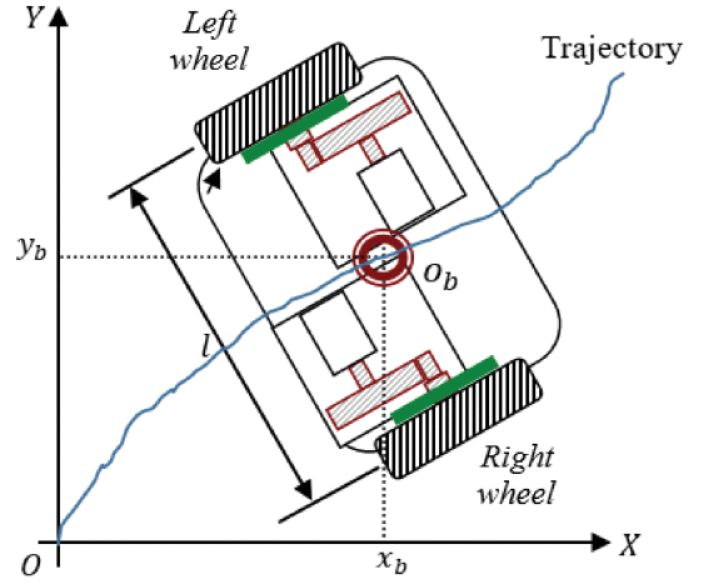
\includegraphics[width=0.6\textwidth]{mob_rob_coo_sys.jpg}
	\caption{Sistema de coordenadas de referencia de un robot móvil con tracción diferencial. $XOY$ muestra el marco de referencia mundial.$(x_{b},y_{b})$ es la coordenada del centro de masa del robot a lo largo de los ejes $X_R$ y $Y_R$, los cuales representan el sistema local de coordenadas del robot \cite{multi-robot_nodate}.}
	\label{fig:coordenadas_rob_mob}
\end{figure}

\section{Localización de robots móviles}
En términos de percepción del entorno, la localización de robots móviles constituye uno de los desafíos fundamentales en la robótica. Este desafío se enfoca en determinar la pose de un robot con respecto a un mapa predefinido del entorno en el que opera. Esta información es crucial para permitir que los robots móviles ejecuten tareas autónomas de manera efectiva, tales como la navegación, manipulación de objetos o inspección de entornos \cite{niko_correll_kinematics}.

En sí, la localización se refiere al proceso de establecer una correspondencia entre el sistema de coordenadas del mapa mundial con las coordenadas locales del sistema del robot. Conocer esta transformación permite que el robot pueda ubicar objetos de interés en su propio marco de referencia, facilitando su navegación. Sin embargo, la pose del robot no se puede detectar directamente, por lo que se emplea una combinación de diferentes sensores para llevar a cabo la localización de robot como cámaras, LiDARs, sistemas de posicionamiento global, entre otros \cite{niko_correll_kinematics}. 

Los problemas de localización varían en dificultad según la naturaleza del entorno y el conocimiento inicial sobre las características del robot. Se distinguen tres tipos de problemas de localización según el conocimiento de la pose del robot: localización local, cuando se conoce la pose inicial; localización global, cuando la pose inicial es desconocida; y el desafío de los ``robots secuestrados'', donde el robot es teletransportado durante su operación. Otro factor que tiene un impacto en la dificultad de localización es si el entorno es dinámico o estático, así como si el algoritmo de localización controla o no el movimiento del robot. Además, la cantidad de robots involucrados también puede representar un desafío adicional, ya que un mayor número de robots aumenta la complejidad del proceso de localización \cite{thrun_probabilistic_2005}.

\section{Localización y Mapeo Simultáneo (SLAM)}
Un desafío central en la robótica móvil es la construcción de un mapa del entorno desconocido mientras simultáneamente se localiza la propia posición del robot dentro de ese mapa. A esta problemática se le denomina localización y mapeo simultaneo o SLAM, por sus siglas en inglés, y a menudo se considera un problema de la clase ``huevo y la gallina'' debido a su estrecha interrelación. Esto pues, la precisión de la localización del robot depende del mapa que esté construyendo, y la precisión del mapa depende de la posición precisa del robot en el entorno \cite{corke_robotics_2017}. 

Para resolver esta problemática, los sistemas de robots móviles emplean una variedad de sensores para recopilar información del entorno y estimar tanto la posición del robot como la estructura del mapa. Una vez se recopilan los datos crudos obtenidos de los sensores, estos son procesados y fusionados para crear mediciones más confiables. Se utiliza algún algoritmo de localización para estimar la posición y orientación del robot en el entorno. Este algoritmo puede basarse en técnicas como el filtro de Kalman, el filtro de partículas, el algoritmo de gráficos de pose u otros \cite{corke_robotics_2017}. 

Simultáneamente, se construye el mapa, empleando las mediciones de los sensores y las estimaciones de la posición del robot. Para esto, se requiere la integración de las observaciones sensoriales en un marco de referencia común. A medida que el robot se mueve, se recopilan más datos por lo que el algoritmo escogido actualiza el mapa y la estimación de la posición del robot constantemente. En algunos casos, se pueden emplear algoritmos de optimización para mejorar la distribución de las características del mapa del entorno y la estimación de la posición del robot. El proceso de SLAM es iterativo y complejo. Como se observa en la Figura \ref{fig:SLAM}, la información odométrica cruda recolectada por el sistema de sensores de un robot móvil no proporciona una representación precisa del mapa del entorno. Sin embargo, mediante la aplicación de algoritmos de mapeo y localización, esta información odométrica se fusiona entre sí para generar un mapa representativo del entorno circundante \cite{thrun_probabilistic_2005}. 

\begin{figure}[H]
	\centering
	\begin{subfigure}{0.5\textwidth}
		\centering	
		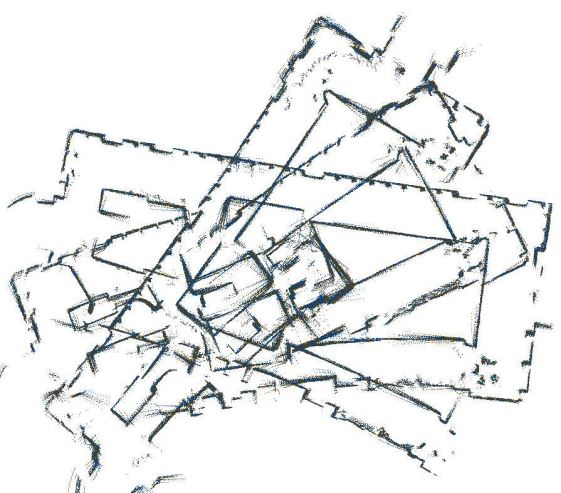
\includegraphics[width=1\linewidth]{mapeo_malo.jpg}
		\caption{Mapeo de entorno utilizando información odométrica cruda.}
	\end{subfigure}
	
	\begin{subfigure}{0.5\textwidth}
		\centering
		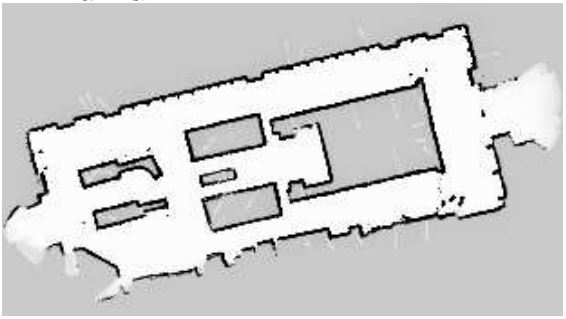
\includegraphics[width=1\linewidth]{mapeo_bueno.jpg}
		\caption{Mapeo de entorno después de fusionar la información odométrica con algoritmo.}
	\end{subfigure}
	
	\caption{Visualización del proceso de SLAM \cite{thrun_probabilistic_2005}.}
	\label{fig:SLAM}
\end{figure}
\section{Filtro de Kalman y filtro de Kalman extendido (EKF)}
El Filtro de Kalman es un algoritmo recursivo utilizado para estimar el estado de un sistema dinámico lineal en presencia de ruido. Cuenta con dos etapas principales: la etapa de predicción, donde se estima el esstao futuro del sistema utilizando el modelo dinámico y la estimación del estado actual, y la etapa de actualización, donde se ajusta la predicción con nuevas mediciones para minimizar el error en la estimación. Este filtro es ideal para sistemas lineales donde las ecuaciones del modelo y las mediciones se describen mediante relaciones lineas. Además, funciona bajo el supuesto de que tanto el proceso como el ruido de las mediciones siguen una distribución normal gaussiana. 


Cuando el sistema no es lineal, se utiliza el Filtro de Kalman Extendido (EKF, por sus siglas en inglés), una extensión del filtro de Kalman clásico. El EKF se utiliza para estimar el estado de un sistema dinámico en presencia de ruido y no linealidades. Este algoritmo funciona iterativamente, actualizando continuamente las estimaciones del estado del sistema a medida que se reciben nuevas mediciones, utilizando una versión linealizada del modelo del sistema. Al igual que el Filtro de Kalman Clásico, el EKF opera bajo dos etapas principales: la etapa de predicción y la etapa de actualización \cite{corke_robotics_2017}. 

En la primera etapa, se predice el estado actual del sistema utilizando el modelo dinámico del mismo y el estado anterior estimado. Junto con la predicción del estado, se predice su covarianza (la incertidumbre en la estimación). En la segunda etapa, se incorporan las nuevas mediciones al estado predicho para mejorar la precisión de la estimación. Se calcula la ganancia de Kalman, que determina cuánta confianza se tiene en la estimación del estado del sistema en función de la diferencia entre las mediciones reales y las predichas por el algoritmo. Finalmente, se utiliza esta ganancia para corregir la estimación del estado del sistema utilizando las mediciones disponibles de tal manera que se minimice el error de la estimación del estado \cite{corke_robotics_2017}.

Esta técnica de estimación es especialmente útil cuando el modelo del sistema y las mediciones no son lineales, lo que lo hace adecuado para sistemas como los robots móviles. Por esta razón, el EKF se utiliza en el contexto de SLAM para estimar la posición del robot en un entorno desconocido mientras construye un mapa del mismo. Siguiendo la metodología anteriormente expuesta, el EKF estima la posición y la orientación del robot en función de las mediciones odométricas y las lecturas de los sensores. A medida que el robot se mueve, se recopilan los datos de sus sensores para crear el mapa del entorno y corregir las estimaciones anteriores de la posición y orientación del mismo. Por medio de la ganancia de Kalman se compensa el error debido a pequeñas desviaciones en la rotación de las ruedas o deslizamientos en las mismas, mejorando así la precisión de la localización del robot y el mapa generado \cite{thrun_probabilistic_2005}.

\section{\textit{Light Detection and Ranging} (LiDAR)}
Los LiDAR son sistemas de teledetección que emplean pulsos de luz láser para medir distancias. Estos dispositivos emiten, de manera individual o continua, pulsos láser dirigidos hacia el objetivo que se va a medir. Al emitir un pulso láser, un circuito interno de sincronización se activa instantáneamente. Se mide el tiempo entre la emisión del pulso láser y su retorno al receptor. Los sensores receptores, al detectar la luz láser reflejada por el objetivo detienen el contador. El número de pulsos de reloj registrados durante la fase de emisión y detección es empleado para calcular la distancia hacia el objetivo. Esta tecnología es ampliamente utilizada en mediciones topográficas para generar mapas de alta resolución del terreno o la superficie. Además, son empleados en vehículos autónomos para la detección y percepción del entorno \cite{lidar}.

Esta tecnología puede clasificarse en dos tipos principales: el escáner LiDAR de una sola línea y el escáner LiDAR multilínea. El primero se utiliza para medir distancias con precisión en una dimensión específica, mientras que el segundo combina múltiples planos de escaneo para capturar mediciones en varias direcciones simultáneamente. Este último, emite pulsos láser en varias direcciones mientras gira y es utilizado en vehículos autónomos para resolver la problemática de SLAM y ofrecer un modelado del entorno más preciso \cite{lidar}.

\begin{figure}[H]
	\centering
	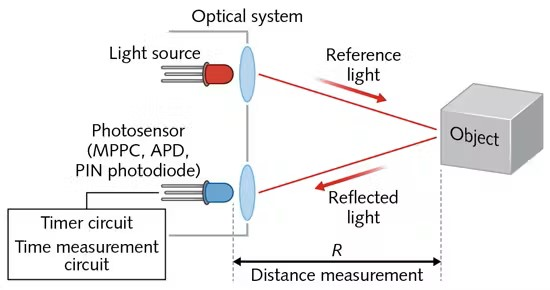
\includegraphics[width=0.65\textwidth]{lidar.jpg}
	\caption{Funcionamiento LiDAR \cite{lidar}.}
	\label{fig:lidar}
\end{figure}

\section{Sensores de distancia por tiempo de vuelo}
Como su nombre lo indica, estos sensores emplean la tecnología de \textit{Time-of-Flight} (ToF) para medir la distancia entre el sensor y un objeto. El principio de funcionamiento se basa en la velocidad de la luz. En sí, el sensor posee un emisor láser que cada cierto tiempo envía fotones que son reflejados por un objeto y detectados por el receptor. La diferencia de tiempo entre la emisión y la recepción proporciona la distancia real del objetivo en milímetros con una alta precisión. Los  sensores ToF ofrecen una rápida respuesta independientemente del tamaño y color del objeto. Son empleados en una amplia gama de aplicaciones, como sistemas de detección de obstáculos, medición de niveles de líquido, reconocimiento de gestos en cámaras y sistemas de seguridad automotriz \cite{tof}.

\section{Sensores de distancia por triangulación}
Los sensores de distancia basados en triangulación utilizan la geometría de triángulos para calcular la distancia a un objeto. En este sistema, un emisor láser proyecta un haz de luz infrarroja hacia el objeto, y la luz reflejada regresa y pasa a través de una lente que enfoca el haz en un detector, donde se registra el punto de incidencia. Este proceso forma dos triángulos similares. El primero se define por la distancia fija entre el emisor láser y el centro óptico de la lente, y la distancia desconocida al punto de reflexión en el objeto. Mientras que el segundo se establece entre el centro óptico de la lente y el plano del detector, junto con la distancia al punto donde el haz de luz reflejado incide sobre el detector.

\begin{figure}[H]
	\centering
	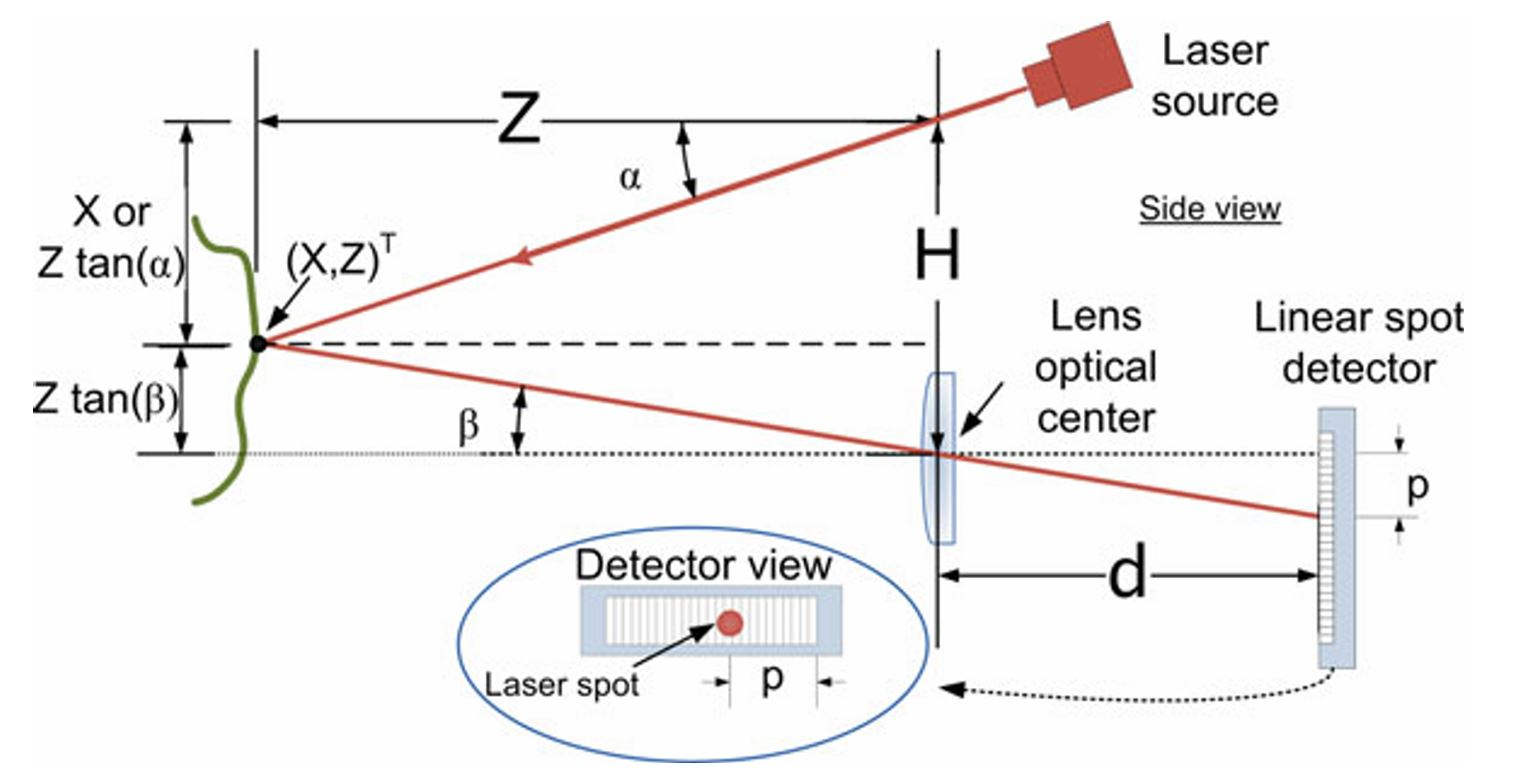
\includegraphics[width=0.75\textwidth]{triangulation.jpg}
	\caption{Diagrama esquemático de un sensor de distancia basado en triangulación. La distancia fija $H$ representa la línea base entre el emisor láser y el centro óptico de la lente, mientras que $d$ es la distancia entre la lente y el detector. El ángulo de proyección del haz láser hacia el objeto se denota como $\alpha$, y el ángulo de recolección $\beta$ se calcula en función de $d$ y la posición $p$ del punto láser en el detector. La ubicación del punto $[X,Z]^T$ se determina  a partir de la línea base $H$, el ángulo de proyección $\alpha$, y el ángulo de recolección $\beta$ \cite{drouin2020}.}
	\label{fig:triangulation}
\end{figure}

A medida que el objeto se aproxima o se aleja, el ángulo reflejado cambia, desplazando el punto de impacto en el detector. Al conocer la distancia fija entre el emisor y el detector y aplicando trigonometría, el sistema puede calcular con precisión la distancia al objeto. Esta técnica permite obtener mediciones precisas a distancias cortas y medias.


\section{Vehículo diferencial \textit{Pololu 3pi+ 32U4}}
El vehículo diferencial Pololu 3pi+ 32U4 es un pequeño robot móvil, con un diámetro nominal de 9.7 cm, manufacturado por Pololu Corporation. Está diseñado para ser un robot de tipo diferencial, por lo que emplea dos ruedas motorizadas independientes para controlar su movimiento. Esto le permite moverse con facilidad y realizar maniobras precisas al variar la velocidad de cada rueda. Una característica notable del robot es que en su núcleo se encuentra un microcontrolador AT-mega32U4 AVR de Microchip, el cual proporciona capacidad de procesamiento y control. Se puede programar utilizando el entorno de desarrollo integrado IDE de Arduino, lo que lo hace accesible para implementar distintos algoritmos de control \cite{pololu}.  

Cuenta con una variedad de sensores, que incluyen una unidad de medición inercial completa (acelerómetro, giroscopio y magnetómetro de 3 ejes), cinco sensores de reflectancia orientados hacia abajo para el seguimiento de bordes y sensores de impacto a lo largo de su cara frontal. Dispone de conexión USB para la comunicación con un ordenador, facilitando la programación del mismo en lenguajes como C o C++. Además, ofrece una serie de periféricos de expansión que permite a los usuarios personalizar y ampliar sus capacidades \cite{pololu}.
\begin{figure}[H]
	\centering
	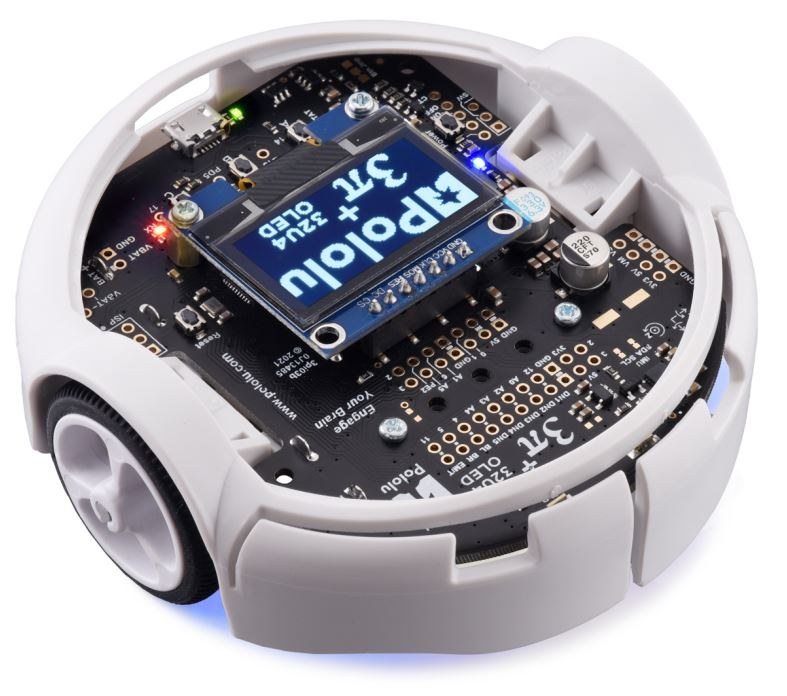
\includegraphics[width=0.5\textwidth]{pololu.jpg}
	\caption{Pololu 3pi+ 32U4 OLED Robot \cite{pololu}.}
	\label{fig:pololu}
\end{figure}

\section{\textit{Universal Asynchronous Receiver-Transmitter} (UART)}

El \textit{Universal Asynchronous Receiver-Transmitter} (UART, por sus siglas en inglés) es uno de los protocolos de comunicación más utilizados en sistemas embebidos debido a su simplicidad. Este protocolo utiliza solo dos cables para transmitir y recibir datos, y opera de manera serial y asíncrona, es decir, no requiere una señal de reloj compartida entre los dispositivos para sincronizar la transmisión de datos. En lugar de eso, la velocidad de transmisión se ajusta configurando la tasa de baudios, la cual define cuántos bits por segundo pueden ser transmitidos y recibidos entre ambos dispositivos \cite{pena_uart_nodate}.

\begin{figure}[H]
	\centering
	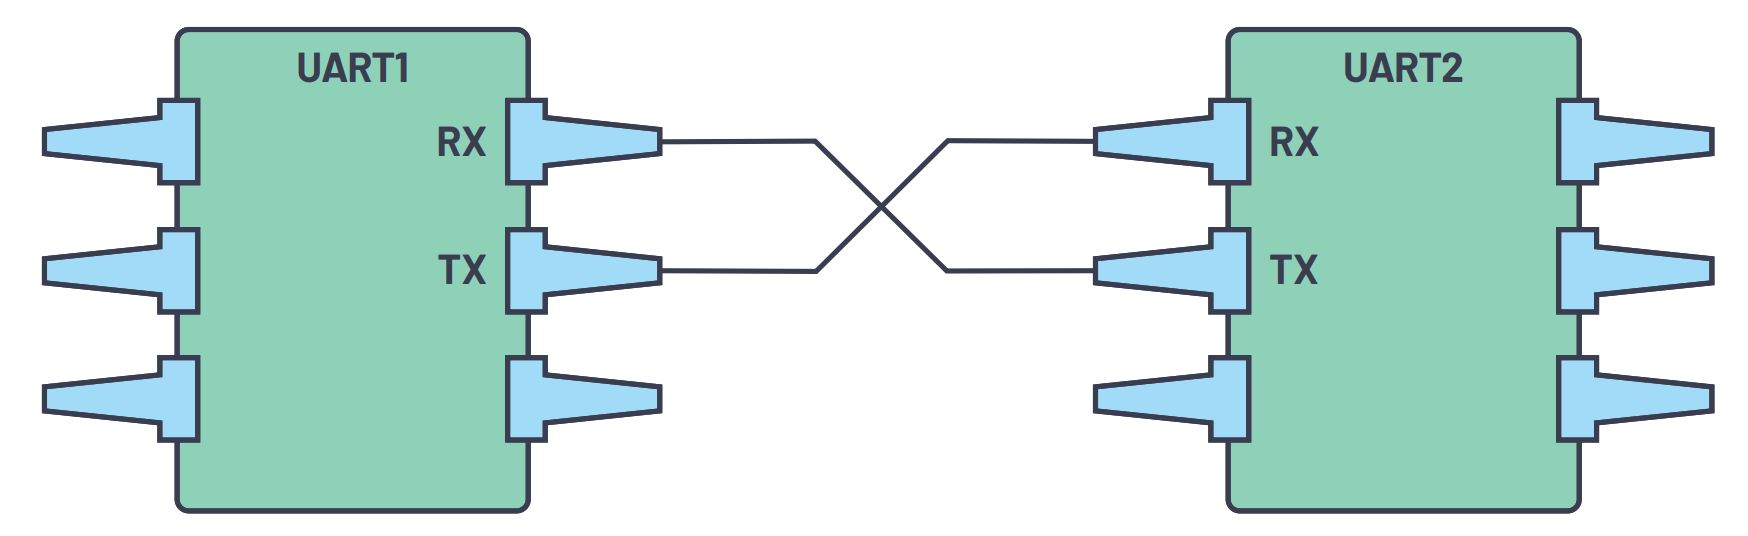
\includegraphics[width=0.7\textwidth]{uart_conexion.jpg}
	\caption{Esquema de comunicación UART entre dispositivos \cite{pena_uart_nodate}.}
	\label{fig:uart_conexión}
\end{figure}

El protocolo UART emplea dos señales principales : transmisión (Tx) y recepción (Rx) . Durante la comunicación, el UART del dispositivo convierte los datos paralelos en un flujo serial de bits, que luego se envían bit a bit a través de la línea Tx a Rx. El UART receptor recibe los datos en serie y los convierte en datos paralelos para el dispositivo receptor. Para que esta comunicación sea efectiva, ambos dispositivos deben estar configurados con la misma velocidad en baudios, lo que asegura que los bits se transmitan y reciban al mismo ritmo, sincronizando el flujo de datos \cite{campbell_basics_2016}.


Existen diferentes modos de comunicación a través de UART:
\begin{itemize}
	\item Simplex: Comunicación unidireccional. Un dispositivo seimpre actúa como transmisor y otro como receptor, sin alternar roles.
	\item Semidúplex: Comunicación bidireccional, pero no simultánea. Ambos dispositivos pueden enviar y recibir datos, pero no al mismo tiempo, se alterna entre transmisión y recepción.
	\item Dúplex completo: Comunicación bidireccional simultánea. Ambos dispositivos pueden enviar y recibir datos al mismo tiempo a través de sus respectivas líneas Tx y Rx.
\end{itemize}

Una característica importante de la comunicación UART es la implementación de una estructura de tramas (\textit{frame protocol}), que añade seguridad y robustez a la transmisión de datos. Cada trama incluye un conjunto de bits que agrupan los datos de manera estructurada con campos por encabezados, datos y verificación de errores, como el \textit{Cyclic Redundancy Check} (CRC) \cite{pena_uart_nodate}. Este protocolo asegura que los datos sean recibidos de manera confiable, y permite a los diseñadores personalizar los encabezados y finales de cada trama para adaptarse a los requisitos específicos de la aplicación. En la Figura \ref{fig:uart_frame} se muestra un ejemplo de cómo se estructura una trama UART.

\begin{figure}[H]
	\centering
	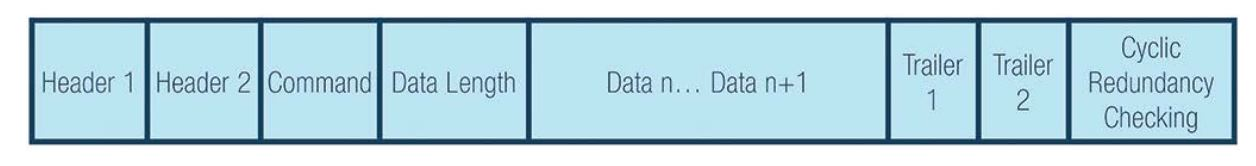
\includegraphics[width=0.8\textwidth]{uart_protocol.jpg}
	\caption{Ejemplo de protocolo de trama UART. \cite{pena_uart_nodate}.}
	\label{fig:uart_frame}
\end{figure}
	\fi
\fi

% CAPÍTULOS
% ------------------------------------------------------------------------------
\newpage
\ifdefined\parpordefecto
	\defaultparformat{j-capitulos}
\else
	\definecolor{celeste}{RGB}{166, 201, 236}
\definecolor{azul1}{RGB}{218, 233, 248}
\definecolor{azul2}{RGB}{192, 230, 245}
\definecolor{azul3}{RGB}{148, 220, 248}
\definecolor{azul4}{RGB}{97, 203, 243}
\definecolor{azul5}{RGB}{68, 179, 225}
\definecolor{azul6}{RGB}{100, 149, 237}
\definecolor{azul7}{RGB}{84, 127, 222}
\definecolor{azul8}{RGB}{77, 147, 217}
\definecolor{azul9}{RGB}{0, 134, 234}
\definecolor{azul10}{RGB}{0, 120, 210}

\chapter{Validación de sensor de distancia tipo láser}

En este capítulo se presentan las alternativas de sensores de distancia tipo láser consideradas y la validación de la selección del sensor más adecuado para la futura implementación de algoritmos de exploración y mapeo de entornos en agentes robóticos móviles. Cada uno de los sensores analizados presenta ventajas específicas, por lo que, con el fin de identificar aquel que mejor se adaptara a las necesidades de esta aplicación, se realizó un \textit{trade study} en el cual se evaluaron diversos parámetros y especificaciones de cada uno de estos. Este análisis comparativo asegura que la elección final ofrezca el mejor rendimiento posible según criterios relevantes para la aplicación.

\section{Sensores de distancia tipo láser considerados}
Las opciones de sensores de distancia tipo láser consideradas para este trabajo fueron: el módulo VL53L0X, el LiDAR FHL-LD20 y el YDLIDAR Tmini Pro. Estos sensores fueron seleccionados estratégicamente para analizar dos tecnologías de medición diferentes: triangulación y tiempo de vuelo (ToF, por sus siglas en inglés). Ambas tecnologías han demostrado ser altamente efectivas en la obtención de mediciones de distancia para aplicaciones de navegación autónoma, haciendo que los sensores que las utilizan sean candidatos adecuados para la aplicación prevista.

\subsection{Sensor VL53L0X}
El sensor de distancia láser VL530X de STMicroelectronics \cite{stmicroelectronics_vl53l0x_2016} es un módulo compacto con microcontrolador integrado que utiliza la tecnología de medición por tiempo de vuelo para obtener mediciones precisas, independientemente de la reflectancia del objetivo. Es capaz de medir distancias con precisión en un rango de 50 mm a 2 m. Una  característica destacada de este sensor es su emisor láser de cavidad vertical de 940 nm, el cual es completamente invisible para el ojo humano durante su funcionamiento. 
 
Con un campo de visión (FoV) típico de 25°, el sensor integra una avanzada matriz SPAD, capaz de detectar fotones individuales incluso en condiciones de luz extremadamente débil. Esta característica junto con sus filtros anti-infrarrojos, mejora significativamente la sensibilidad y precisión de las mediciones en entornos con niveles altos de luz infrarroja. Adicionalmente, su interfaz $I^2C$ estándar facilita el control y transferencia de datos, lo que simplifica su integración en proyectos electrónicos. Por estas razones, es ampliamente utilizado en aplicaciones como prevención de colisiones, detección de bordes, o en sistemas de auto-enfoque en cámaras digitales \cite{stmicroelectronics_vl53l0x_2016}.

\subsection{LiDAR FHL-LD20}

El LiDAR FHL-LD20, desarrollado por youyeetoo Tech \cite{youyeetoo_tech_ld20_nodate}, es un sensor omnidireccional de 360° que emplea tecnología de triangulación para escanear su entorno. Una vez recopilados los datos de distancia, el sensor combina estos valores con los ángulos medidos por la unidad de medición angular para generar una nube de puntos, que puede utilizarse para crear un mapa detallado del contorno circundante. Además, cuenta con un CCD fotosensible de alto rendimiento, el cual le permite medir distancias con precisión en un rango de 100 mm a 8 m. 

El núcleo de medición de distancia del FHL-LD20 permite capturar 4000 puntos por segundos, lo que facilita la actualización del entorno capturado. Esta capacidad, junto con la modulación de la velocidad del motor, mejora la cobertura del sensor y reduce los puntos ciegos en distintos entornos. Adicionalmente, su comunicación serial UART simplifica la integración del LiDAR en una amplia variedad de aplicaciones, como la navegación autónoma en robots móviles, la reconstrucción de mapas 2D y la elusión de obstáculos \cite{youyeetoo_tech_ld20_nodate}.

\subsection{YDLIDAR Tmini Pro}

El YDLIDAR Tmini Pro es un LiDAR 2D de 360° desarrollado por EAI Technology \cite{eai_technology_ydlidar_2022}. Emplea el principio de tiempo de vuelo para lograr mediciones de distancia con alta precisión. Durante la medición, su estructura mecánica gira 360 grados, lo que le permite obtener información continua de ángulos y realizar un escaneo completo del entorno. Entre sus características destacadas se encuentra su resistencia al polvo y al agua, lo que lo hace adecuado para operar en condiciones ambientales adversas.

Junto a esto, su tamaño compacto facilita su integración a otros sistemas, optimizando la estructura espacial en una amplia variedad de aplicaciones. Esto lo hace adecuado para pruebas en diversos escenarios. Utiliza comunicación serial UART para transmitir los datos de medición, lo que simplifica su conexión con sistemas de procesamiento. Con un rango de medición de 20 mm a 12 m, el YDLIDAR Tmini Pro es empleado en navegación y elusión de obstáculos en robots de servicio doméstico y aspiradoras robot, mejorando su eficiencia y capacidad de respuesta en entornos complejos \cite{eai_technology_ydlidar_2022}.

\section{Selección del sensor de distancia tipo láser}
Los sensores descritos en la sección anterior fueron evaluados considerando sus diferencias en metodología de medición y cantidad de datos generados. Aunque los tres sensores comparten el mismo propósito, estas variaciones presentan ventajas y desventajas específicas en función del objetivo y contexto de cada proyecto. Por esta razón, para realizar una comparación efectiva entre estos, se establecieron distintos criterios que se consideraron fundamentales para el desarrollo de este trabajo.

En el Cuadro \ref{cuadro:criterios} se presentan los criterios empleados en el \textit{trade study} junto con el peso asignado a cada parámetro. Estos pesos fueron determinados mediante el proceso de ponderación por pares, un método utilizado para comparar y sopesar criterios cualitativos y cuantitativos entre sí. Para este estudio, se consideraron 10 criterios para asegurar una decisión fundamentada al escoger el sensor.

\begin{table}[H]
	\centering
	\begin{tabular}{|l|r|}
		\hline
		\multicolumn{1}{|c|}{\textbf{Criterios}}&\multicolumn{1}{|c|}{\textbf{Peso}}\\ 
		\hline
		Costo&$10\%$\\
		\hline
		Disponibilidad&$15\%$\\
		\hline
		Precisión&$6\%$\\
		\hline
		Rango de medición&$7\%$\\
		\hline
		Parámetros eléctricos&$5\%$\\
		\hline
		Velocidad de medición&$6\%$\\
		\hline
		Tamaño&$6\%$\\
		\hline
		Masa&$8\%$\\
		\hline
		Operatividad en aplicaciones deseadas&$22\%$\\
		\hline
		Adaptabilidad a robots móviles&$15\%$\\
		\hline
	\end{tabular}
	\caption{Criterios de comparación.} 
	\label{cuadro:criterios}
\end{table}

El método de ponderación por pares emplea una matriz de comparaciones (ver Cuadro \ref{cuadro:matrizPP}) para evaluar la importancia relativa entre cada par de criterios. Primero, se calcula la media geométrica de los valores en cada fila de la matriz. Luego, estos valores se normalizan para obtener los factores de ponderación, garantizando que la suma total sea igual a 1 \cite{fatchurrahman_light_2016}. Los valores para las comparaciones se seleccionan dentro de un intervalo 1 a 9, como se describe en el Cuadro \ref{cuadro:valoresPP}.

\begin{table}[H]
	\centering
	\rotatebox{90}{
		\resizebox{0.98\textheight}{!}{
			\begin{tabular}{|c|c|c|c|c|c|c|c|c|c|c|c|c|}
				\hline
				&Costo&Disponibilidad&Precisión&\makecell{Rango\\de medición}&\makecell{Parámetros\\eléctricos}&\makecell{Velocidad\\de medición}&Tamaño&Peso&Operatividad&Adaptabilidad&\makecell{Media\\ Geométrica}&Masa\\
				\hline
				Costo&1&1/4&1/2&3&2&5&4&4&1/5&1/3&1.1487&0.1019
				\\
				\hline
				Disponibilidad&4&1&3&2&2&4&3&3&1/3&1/4&1.6438&0.1458
				\\
				Precisión&2&1/3&1&7&3&1&1/4&1/4&1/8&1/6&0.6700&0.0594
				\\
				\hline
				\makecell{Rango\\de medición}&1/3&1/2&1/7&1&5&1/3&5&5&1/3&1/4&0.7794&0.0691
				\\
				\hline
				\makecell{Parámetros\\eléctricos}&1/2&1/2&1/3&1/5&1&1/5&2&1/2&1/2&3&0.5887&0.0522
				\\
				\hline
				\makecell{Velocidad\\de medición}&1/5&1/4&1&3&5&1&1/4&1/4&1&1/2&0.6871&0.0609
				\\
				\hline
				Tamaño&1/4&1/3&4&1/5&1/2&4&1&1&1/5&1&0.6960&0.0617
				\\
				\hline
				Masa&1/4&1/3&4&1/5&2&4&1&1&1/3&1&0.8414&0.0746
				\\
				\hline
				Operatividad&5&3&8&3&2&1&5&3&1&1&2.5313&0.2244
				\\
				\hline
				Adaptabilidad&3&4&6&4&1/3&2&1&1&1&1&1.6917&0.1500
				\\
				\hline
				\multicolumn{11}{|r|}{Suma}&11.2779&1.0000
				\\
				\hline
			\end{tabular}
		}
	}
	\caption{Matriz de comparación por pares.} 
	\label{cuadro:matrizPP}
\end{table}

\begin{table}[H]
	\centering
	\begin{tabular}{|c|l|}
		\hline
		\multicolumn{1}{|c|}{\textbf{Valor}}&\multicolumn{1}{|c|}{\textbf{Descripción}}\\ \hline
		1&Igual importancia\\ \hline
		3&Moderadamente más importante\\ \hline
		5&Fuertemente más importante\\ \hline
		7&Muy fuertemente más importante\\ \hline
		9&Extremadamente más importante\\ \hline
		2,4,6,8&Valores intermedios entre los anteriores\\ \hline
		
	\end{tabular}
	\caption{Escala fundamental de comparación por pares.} 
	\label{cuadro:valoresPP}
\end{table}

\subsection{Criterios para el \textit{Trade Study} de los sensores de distancia tipo láser}
El \textit{trade study} es un método sistemático de toma de decisiones diseñado para identificar la solución técnica más adecuada entre un conjunto de alternativas viables. Este enfoque consiste en evaluar y comparar diferentes opciones en función de una serie de criterios predefinidos, los cuales son ponderados numéricamente según su importancia relativa en el proyecto. A cada criterio se le asigna un peso específico, de manera que las alternativas que satisfacen más plenamente con dicho criterio obtengan una puntuación superior a aquellas que lo satisfacen en menor medida. El Cuadro \ref{cuadro:valoresCompa} muestra las calificaciones posibles al desempeño de cada uno de los criterios evaluados.

\begin{table}[H]
	\centering
	\begin{tabular}{|l|l|}
		\hline
		\multicolumn{1}{|c|}{\textbf{Adjetivos(s)}}&\multicolumn{1}{|c|}{\textbf{Calificación}}\\ \hline
		No aceptable / Nulo&0\\ \hline
		Muy malo / Muy bajo&1\\ \hline
		Malo / Bajo&2\\ \hline
		Moderado / Normal&3\\ \hline
		Bueno / Alto&4\\ \hline
		Muy bueno / Muy Alto&5\\ \hline
		
	\end{tabular}
	\caption{Valores de interés para la comparación.} 
	\label{cuadro:valoresCompa}
\end{table}

\subsubsection{Costo}
Dado que no se contaba con los dispositivos, fue necesario evaluar su compra. Para este criterio, se asignó la ponderación más alta al módulo VL53L0X, cuyo precio aproximo de \$6.00 lo hace más accesible que los otros sensores de distancia. Su precio resulta ser más de diez veces inferior al de los LiDAR evaluados. Cabe señalar que las ponderaciones asignadas a cada sensor en el Cuadro \ref{cuadro:ponderacionCosto} reflejan las limitaciones económicas del proyecto, donde se priorizaron las opciones que se ajustaran al presupuesto disponible. En el Cuadro \ref{cuadro:caracteristicasgenerales} se especifican los precios de los LiDAR, junto con características destacables que serán mencionadas en los criterios de evaluación.

\begin{table}[H]
	\centering
	\begin{tabular}{|l|l|}
		\hline
		\textbf{Alternativa} & \textbf{Costo} \\ \hline
		VL53L0X & 5 \\ \hline
		FHL-LD20 & 3 \\ \hline
		YDLIDAR Tmini Pro & 1 \\ \hline
	\end{tabular}
	\caption{Ponderación de costo.} 
	\label{cuadro:ponderacionCosto}
\end{table}


\subsubsection{Disponibilidad}
Este criterio es considerado uno de los más importantes, ya que la disponibilidad de un sensor influye directamente en diversos aspectos. Por un lado, un sensor que se encuentra ampliamente disponible permite realizar sustituciones rápidas y oportunas cuando sea necesario. Junto a esto, los sensores con amplia disponibilidad suelen ofrecer un mejor soporte técnico, lo que facilita su mantenimiento y desarrollo. En este contexto, como se muestra en el Cuadro \ref{cuadro:ponderacionDisponibilidad}, el módulo VL53L0X recibió la ponderación más alta, ya que es accesible en el mercado local de Guatemala. Es importante señalar que, aunque los otros dos sensores son desarrollados en el extranjero y generan un cargo adicional por envío, también cuentan con un excelente soporte técnico. 

\begin{table}[H]
	\centering
	\begin{tabular}{|l|l|}
		\hline
		\multicolumn{1}{|c|}{\textbf{Alternativas}}&\multicolumn{1}{|c|}{\textbf{Disponibilidad}}\\ \hline
		VL53L0X&5\\ \hline
		FHL-LD20&3\\ \hline
		YDLIDAR Tmini Pro&1\\ \hline
	\end{tabular}
	\caption{Ponderación de disponibilidad.} 
	\label{cuadro:ponderacionDisponibilidad}
\end{table}

\subsubsection{Precisión}
Como se indica en el Cuadro \ref{cuadro:caracteristicasgenerales}, la precisión de cada sensor se presenta dentro de un rango, donde el primer valor refleja la precisión en condiciones óptimas y el segundo corresponde a escenarios menos favorables. Aunque estos valores pueden fluctuar según el entorno donde se utilicen, los rangos proporcionan una idea general de la precisión de cada sensor. En este contexto, se observa que ambos sensores de distancia tipo láser LiDAR tienen una precisión inferior en comparación con el módulo VL53L0X. En particular, el FHL-LD20 muestra la menor precisión entre los tres sensores evaluados, lo que justifica su puntuación en el Cuadro \ref{cuadro:ponderacionPrecision}. 

\begin{table}[H]
	\centering
	\begin{tabular}{|l|l|}
		\hline
		\multicolumn{1}{|c|}{\textbf{Alternativas}}&\multicolumn{1}{|c|}{\textbf{Precisión}}\\ \hline
		VL53L0X&5\\ \hline
		FHL-LD20&3\\ \hline
		YDLIDAR Tmini Pro&4\\ \hline
	\end{tabular}
	\caption{Ponderación de precisión.} 
	\label{cuadro:ponderacionPrecision}
\end{table}

\subsubsection{Rango de medición}
El rango de medición del sensor debe ser adecuado para cubrir las dimensiones del área de trabajo. Puesto que se planea operar en el ecosistema Robotat, que cuenta con una plataforma de 4.8$\times$3.8 m, es importante que el sensor tenga un rango suficiente para medir distancias dentro de este espacio sin restricciones. Además, al considerar su futura integración con robots móviles para el mapeo de entornos, un rango de medición limitado podría restringir significativamente su utilidad. En este contexto, el FHL-LD20 obtiene la ponderación más alta (ver Cuadro \ref{cuadro:ponderacionRango}), ya que tiene la capacidad de cubrir áreas de trabajo moderadamente grandes como la plataforma del Robotat . 

\begin{table}[H]
	\centering
	\begin{tabular}{|l|l|}
		\hline
		\multicolumn{1}{|c|}{\textbf{Alternativas}}&\textbf{\makecell{Rango\\de medición}}\\ \hline
		VL53L0X&2\\ \hline
		FHL-LD20&5\\ \hline
		YDLIDAR Tmini Pro&4\\ \hline
		
	\end{tabular}
	\caption{Ponderación de rango de medición.} 
	\label{cuadro:ponderacionRango}
\end{table}

\subsubsection{Parámetros eléctricos}
El sensor debe ser compatible con el voltaje de operación del sistema en el que se integrará, ya que esto influye directamente en el diseño general del mismo. También, es importante conocer su consumo de corriente para evitar sobrecargas en la fuente de alimentación. En aplicaciones móviles, un sensor con bajo consumo de energía es preferible, ya que extiende el tiempo de funcionamiento y reduce la frecuencia de recargas. Como se muestra en el Cuadro \ref{cuadro:caracteristicasgenerales}, los tres sensores operan con voltajes de alimentación similares. Sin embargo, los sensores LiDAR presentan un mayor consumo de corriente durante su funcionamiento. Aunque este incremento es manejable al integrarlos con otros subsistemas, el módulo VL53L0X destaca por su menor consumo energético, lo cual respalda su puntuación en el Cuadro \ref{cuadro:PE}. 


\begin{table}[H]
	\centering
	\begin{tabular}{|l|l|}
		\hline
		\multicolumn{1}{|c|}{\textbf{Alternativas}}&\textbf{\makecell{Parámetros\\eléctricos}}\\ \hline
		VL53L0X&5\\ \hline
		FHL-LD20&3\\ \hline
		YDLIDAR Tmini Pro&3\\ \hline
	\end{tabular}
	\caption{Ponderación de parámetros eléctricos.} 
	\label{cuadro:PE}
\end{table}


\subsubsection{Velocidad de medición}
Una mayor velocidad de medición permite capturar rápidamente los cambios en el entorno, lo que mejora la capacidad de respuesta en tiempo real. En este aspecto, tanto el sensor LiDAR FHL-LD20 como el YDLIDAR Tmini Pro pueden obtener mediciones a una velocidad de 4000 puntos por segundo, lo que les otorga una alta ponderación en este criterio (ver Cuadro \ref{cuadro:VM}). Por otro lado, la velocidad de medición del módulo VL53L0X depende del modo de operación, con tiempos de respuesta típicos que oscilan entre 30 ms y 200 ms, lo que lo hace más lento en comparación con los otros sensores.


\begin{table}[H]
	\centering
	\begin{tabular}{|l|l|}
		\hline
		\multicolumn{1}{|c|}{\textbf{Alternativas}}&\textbf{\makecell{Velocidad\\de medición}}\\ \hline
		VL53L0X&2\\ \hline
		FHL-LD20&5\\ \hline
		YDLIDAR Tmini Pro&5\\ \hline
	\end{tabular}
	\caption{Ponderación de velocidad de medición.} 
	\label{cuadro:VM}
\end{table}

\subsubsection{Tamaño}
Un sensor compacto se integra más fácilmente en sistemas con espacio limitado como lo podría ser un robot móvil. Un tamaño reducido permite mayor flexibilidad en el diseño estructural del sistema. En este contexto, como se muestra en el Cuadro \ref{cuadro:Tamaño}, el módulo VL53L0X recibió la ponderación más alta. No obstante, los tamaños de los otros dos sensores también son manejables y adecuados para la aplicación en cuestión. 

\begin{table}[H]
	\centering
	\begin{tabular}{|l|l|}
		\hline
		\multicolumn{1}{|c|}{\textbf{Alternativas}}&\multicolumn{1}{|c|}{\textbf{Tamaño}}\\ \hline
		VL53L0X&5\\ \hline
		FHL-LD20&3\\ \hline
		YDLIDAR Tmini Pro&4\\ \hline
	\end{tabular}
	\caption{Ponderación de tamaño.} 
	\label{cuadro:Tamaño}
\end{table}

\subsubsection{Masa}
Cada gramo adicional puede impactar la eficiencia energética y la estabilidad de sistema en el que se integre el sensor. Un sensor liviano reduce la carga que el sistema debe soportar, favoreciendo su rendimiento. Por esta razón, el módulo VL53L0X recibió la mayor ponderación en términos de masa. Sin embargo, las masas de los otros dos sensores también son manejables y adecuados para la aplicación en cuestión, siendo el YDLIDAR Tmini Pro el sensor con menor puntuación debido a su mayor masa (ver Cuadro \ref{cuadro:Masa}).

\begin{table}[H]
	\centering
	\begin{tabular}{|l|l|}
		\hline
		\multicolumn{1}{|c|}{\textbf{Alternativas}}&\multicolumn{1}{|c|}{\textbf{Masa}}\\ \hline
		VL53L0X&5\\ \hline
		FHL-LD20&3\\ \hline
		YDLIDAR Tmini Pro&4\\ \hline
	\end{tabular}
	\caption{Ponderación de masa.} 
	\label{cuadro:Masa}
\end{table}

\subsubsection{Operatividad en aplicaciones deseadas}
Este fue el criterio que se consideró más importante, pues determina cómo el sensor se ajusta a las necesidades específicas de la aplicación. Puesto que se requiere para futuras aplicaciones de mapeo de entornos con robots móviles, la naturaleza unidireccional del módulo VL53L0X afecta su rendimiento en comparación con los otros dos sensores, que son omnidireccionales. Por esta razón, como se muestra en el Cuadro \ref{cuadro:operatividad}, el módulo VL53L0X obtuvo la menor puntuación en comparación a los LIDAR evaluados. El VL53L0X mide distancias en una sola dirección a la vez, lo que implica que para capturar un mapa completo del entorno, el sensor se debe girar o el robot cambiar su orientación. Esto puede complicar la eficiencia en la obtención de datos y aumentar el tiempo necesario para crear un mapa exhaustivo. 

Por otro lado, los sensores omnidireccionales tienen la ventaja de capturar el entorno completo en una sola rotación. Eso reduce significativamente el tiempo necesario para obtener un mapa completo y facilita la interpretación de bordes y esquinas al realizar SLAM. Esta capacidad mejora notablemente la eficiencia en la programación de algoritmos de mapeo y planificación de trayectorias, haciéndolos ideales para aplicaciones de navegación autónoma, evasión de obstáculos y generación de mapas 2D. En contraste, el sensor unidireccional enfrenta desafíos adicionales en términos de localización y mapeo, dado que requiere múltiples capturas para obtener una visión completa del entorno. 


\begin{table}[H]
	\centering
	\begin{tabular}{|l|l|}
		\hline
		\multicolumn{1}{|c|}{\textbf{Alternativas}}&\textbf{\makecell{Operatividad\\en aplicaciones\\deseadas}}\\ \hline
		VL53L0X&1\\ \hline
		FHL-LD20&5\\ \hline
		YDLIDAR Tmini Pro&5\\ \hline
	\end{tabular}
	\caption{Ponderación de operatividad en aplicaciones deseadas.} 
	\label{cuadro:operatividad}
\end{table}

\subsubsection{Adaptabilidad a robots móviles}
Este criterio, considerado como el segundo en importancia, evalúa la facilidad de integración y el desempeño del sensor en sistemas robóticos. Este criterio hace énfasis en la facilidad de montaje y mantenimiento al integrar el sensor al diseño estructural de distintos sistemas robóticos, asegurando que no interfieran con otros componentes estructurales. También, toma en cuenta el campo de visión, que determina la cobertura del entorno: un campo de visión más amplio proporciona una visión más completa y detallada. Finalmente, se analiza la robustez y resistencia del sensor frente a condiciones operativas adversa. 

En este contexto, dado que se planea utilizar los sensores en aplicaciones futuras con robots móviles, la naturaleza unidireccional del módulo VL53L0X exige la instalación de al menos cinco sensores para cubrir múltiples direcciones y recabar suficientes características del entorno. Otra alternativa sería implementar un sistema de rotación para obtener una cobertura completa sin la necesidad de instalar más de uno, lo que añadiría complejidad al diseño. En contraste, los sensores LiDAR están diseñados para ser montados en diversas posiciones y orientaciones, lo cual facilita su integración en robots móviles y ofrece una cobertura más amplia del entorno. Además, su capacidad para operar en diversas condiciones ambientales, tanto en interiores como exteriores, y su versatilidad en aplicaciones, les otorgan una puntuación superior que el módulo VL53L0X (ver Cuadro \ref{cuadro:adaptabilidad}).

\begin{table}[H]
	\centering
	\begin{tabular}{|l|l|}
		\hline
		\multicolumn{1}{|c|}{\textbf{Alternativas}}&\textbf{\makecell{Adaptabilidad\\a robots móviles}}\\ \hline
		VL53L0X&2\\ \hline
		FHL-LD20&4\\ \hline
		YDLIDAR Tmini Pro&5\\ \hline
	\end{tabular}
	\caption{Ponderación de adaptabilidad a robots móviles.} 
	\label{cuadro:adaptabilidad}
\end{table}

\begin{table}[H]
	\centering
	\resizebox{\textwidth}{!}{
	\begin{tabular}{|c|l|l|l|}
		\hline
		&\multicolumn{1}{|c|}{\textbf{VL53L0X}}&\multicolumn{1}{|c|}{\textbf{FHL-LD20}}&\multicolumn{1}{|c|}{\textbf{YDLIDAR Tmini Pro}}\\
		\hline
		\multicolumn{1}{|c|}{\textbf{Precio}}&\$6.00&\$60.00&\$100.00\\
		\hline
		\multicolumn{1}{|c|}{\textbf{Disponibilidad}}&Guatemala&Estados Unidos&Estados Unidos\\
		\hline
		\multicolumn{1}{|c|}{\textbf{Precisión}}&$\pm$ 3 mm a $\pm$ 10 mm&$\pm$ 10 mm a $\pm$ 20 mm&$\pm$ 25 mm a $\pm$ 50 mm\\
		\hline
		\multicolumn{1}{|c|}{\textbf{Rango de medición}}& 50 mm a 2 m& 100 mm a 8 m&20 mm a 12 m\\
		\hline
		\multicolumn{1}{|c|}{\textbf{Parámetros eléctricos}}& DC 3.3 V @ 20 mA & \multicolumn{1}{|l|}{\makecell{DC 5 V @ 300 mA\\$i_{inrush} \leq 1.0$ A}} & \multicolumn{1}{|l|}{\makecell{DC 5 V @ 340 mA\\$i_{inrush} \leq 1.0$ A}}\\
		\hline
		\multicolumn{1}{|c|}{\textbf{Velocidad de medición}}& 30 ms a 200 ms & 4000 puntos/s & 4000 puntos/s\\
		\hline
		\multicolumn{1}{|c|}{\textbf{Tamaño}}& 4.4 $\times$ 2.4 $\times$ 1.0 mm & 96.3 $\times$ 59.8 $\times$ 38.8 mm & 38.6 $\times$ 38.6 $\times$ 33.4 mm\\
		\hline
		\multicolumn{1}{|c|}{\textbf{Peso}}& 2.0 g & 100.4 g & 45.0 g\\
		\hline
		\textbf{\makecell{Operatividad en\\ aplicaciones deseadas}}& Unidireccional & Omnidireccional & Omnidireccional\\
		\hline
		\textbf{\makecell{Adaptabilidad a\\robots móviles}}& $I^2C$ & UART & UART\\
		\hline
	\end{tabular}}
	\caption{Características de los sensores analizados.} 
	\label{cuadro:caracteristicasgenerales}
\end{table}

\subsection{Resultados del \textit{trade study}}
Una vez definidos los pesos y ponderaciones de los criterios presentados previamente, se elaboró un esquema de ponderación para obtener los resultados del estudio comparativo. En la Figura \ref{fig:graf_trade_study}, el gráfico de barras apiladas ilustra el valor total de cada alternativa a través de la longitud de la barra segmentada. Cada segmento de la barra representa un criterio evaluado (ver Figura \ref{fig:legend_graf_trade_study}), y su longitud indica la magnitud de la ponderación obtenida. De acuerdo con la puntuación final, se concluyó que el LiDAR FHL-LD20 era la opción más adecuada como sensor de distancia tipo láser. Por lo tanto, se seleccionó para utilizarlo en investigaciones con robots móviles dentro del ecosistema Robotat. Cabe señalar que en el Cuadro \ref{cuadro:ponderacion_individual} se resume la ponderación individual obtenida por cada sensor de acuerdo con los criterios mencionados anteriormente.

\begin{figure}[H]
	\centering
	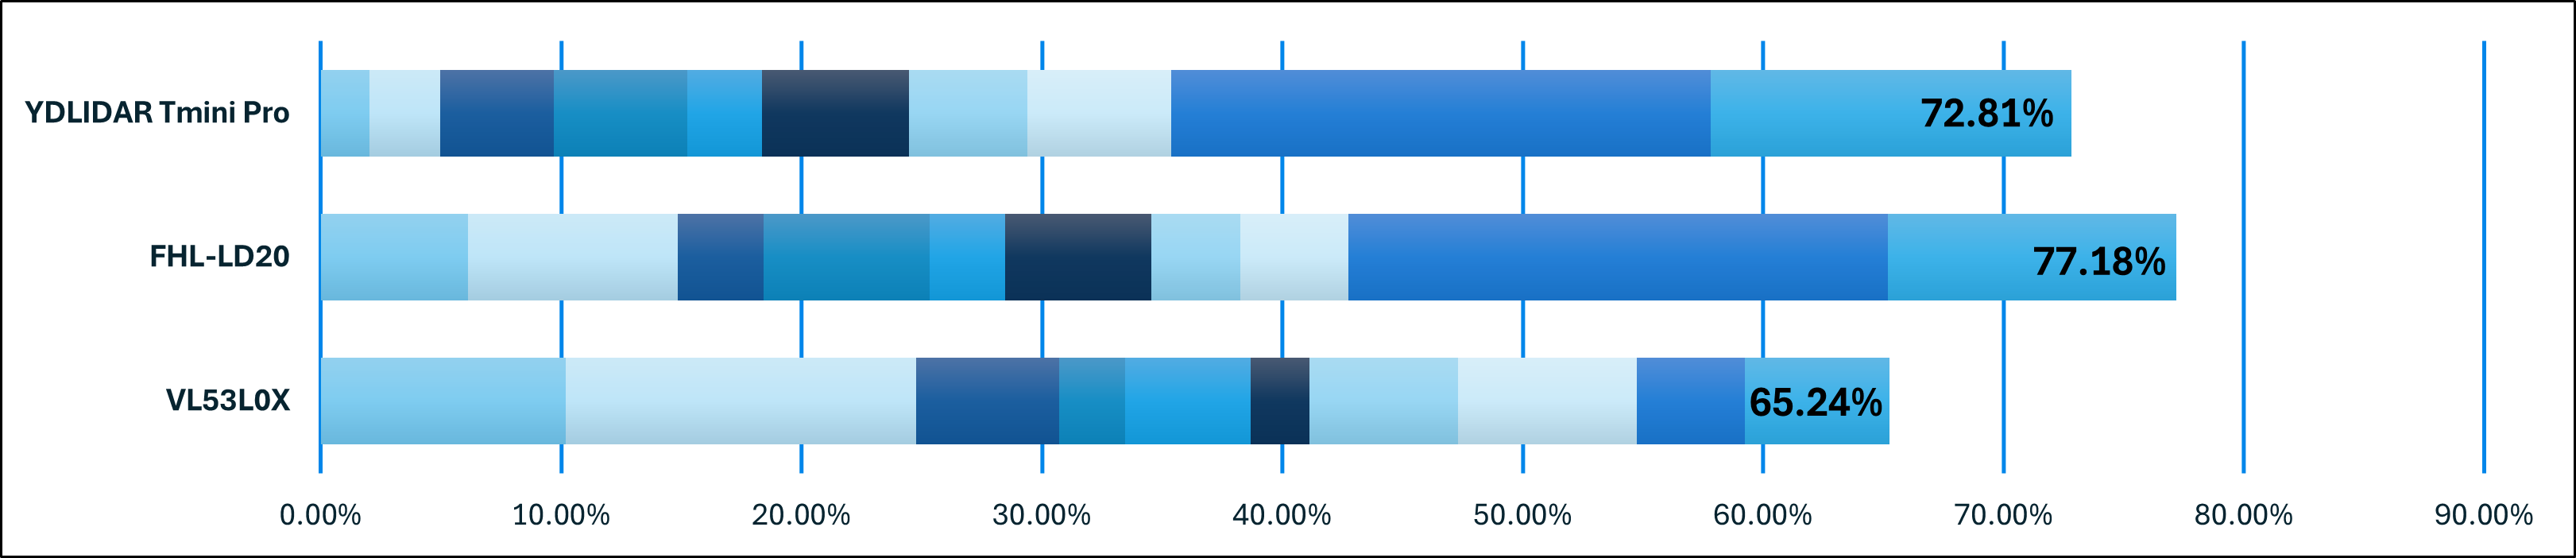
\includegraphics[width=1\textwidth]{trade_study.png}
	\caption{Resultados del \textit{trade study}.}
	\label{fig:graf_trade_study}
\end{figure}

\begin{figure}[H]
	\centering
	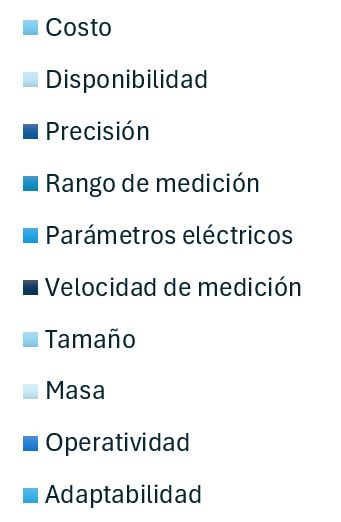
\includegraphics[width=0.25\textwidth]{parametros_tradestudy.jpg}
	\caption{Leyenda del gráfico de barras segmentadas.}
	\label{fig:legend_graf_trade_study}
\end{figure}

\begin{table}[H]
	\centering
	\begin{tabular}{|l|r|r|r|}
		\hline
		\multirow{2}{6.5cm}{\centering\textbf{Criterios}}&\multicolumn{1}{|c|}{\textbf{VL53L0X}}&\multicolumn{1}{|c|}{\textbf{FHL-LD20}}&\multicolumn{1}{|c|}{\textbf{\makecell{YDLIDAR\\Tmini Pro}}}\\
		\cline{2-4}
		&\multicolumn{1}{|c|}{Pesos}&\multicolumn{1}{|c|}{Pesos}&\multicolumn{1}{|c|}{Pesos}\\
		
		\hline
		Costo&$10.19\%$&$6.11\%$&$2.04\%$\\
		\hline
		Disponibilidad&$14.57\%$&$8.74\%$&$2.91\%$\\
		\hline
		Precisión&$5.94\%$&$3.56\%$&$4.75\%$\\
		\hline
		Rango de medición&$2.76\%$&$6.91\%$&$5.53\%$\\
		\hline
		Parámetros eléctricos&$5.22\%$&$3.13\%$&$3.13\%$\\
		\hline
		Velocidad de medición&$2.44\%$&$6.09\%$&$6.09\%$\\
		\hline
		Tamaño&$6.17\%$&$3.70\%$&$4.94\%$\\
		\hline
		Masa&$7.46\%$&$4.48\%$&$5.97\%$\\
		\hline
		Operatividad en aplicaciones deseadas&$4.49\%$&$22.44\%$&$22.44\%$\\
		\hline
		Adaptabilidad a robots móviles&$6.00\%$&$12.00\%$&$15.00\%$\\
		\hline
		\multicolumn{1}{|r|}{\textbf{Total}}&\textbf{$65.24\%$}&\textbf{$77.18\%$}&\textbf{$72.81\%$}\\
		\hline
	\end{tabular}
	\caption{Ponderación individual de los sensores evaluados según criterios establecidos.} 
	\label{cuadro:ponderacion_individual}
\end{table}

\chapter{Lectura e interpretación de datos extraídos del LiDAR FHL-LD20}
Este capítulo aborda el funcionamiento y la interpretación de datos del sensor LiDAR FHL-LD20. Se detalla el formato de los paquetes de datos enviados por el sensor, y se describe cómo se captura y procesa esta información utilizando software como Matlab y Python. Además, se presenta la aplicación desarrollada para que el usuario comprenda como operar el sensor y utilizar de manera efectiva los datos que proporciona.

\section{Funcionamiento del sensor de distancia FHL-LD20}
Esta sección se centra en el funcionamiento del sensor FHL-LD20, detallando sus características técnicas, protocolo de comunicación y la estructura de los datos que transmite. Se exploran los principios de operación que permiten al sensor capturar y transmitir información de manera eficiente. La comprensión de estos aspectos es fundamental para integrar y utilizar el sensor de manera efectiva en aplicaciones que requieran mediciones precisas. 
\subsection{Características generales}
El sensor de distancia tipo láser FHL-LD20, fabricado por Youyeetoo, está diseñado para capturar datos en un plano bidimensional, generalmente en orientación horizontal. Utiliza un láser infrarrojo con una longitud de onda que varía entre 775 nm y 800 nm, siendo 793 nm el valor típico. Su campo de visión (FOV, por sus siglas en inglés) abarca una sección circular de 360° con un radio que varía entre 100 mm y 8 m. Además, cuenta con un motor eléctrico integrado que hace girar la ventana óptica de emisión y recepción del láser, permitiendo cubrir un ángulo de medición en todo el plano horizontal. En el Cuadro \ref{cuadro:parametrosrendi} se presentan a algunos parámetros relevantes del sensor.

\begin{table}[H]
	\centering
	\begin{tabular}{|l|l|} 
		\hline
		\multicolumn{2}{|c|}{Parámetros de rendimiento}\\
		\hline
		\multicolumn{1}{|l|}{Resolución angular}& 0.54°\\
		\hline
		\multicolumn{1}{|l|}{\textit{Pitch}}& 0°$\sim$1.0°\\
		\hline		
		\multicolumn{1}{|l|}{\textit{Yaw}}& -0.5°$\sim$0.5°\\
		\hline
		\multirow{2}{*}{Tiempo de arranque}&$\leq$ 3.4 s\\
		&Típico de 3 s\\
		\hline
		\multicolumn{1}{|l|}{Frecuencia de escaneo}& 6 Hz $\pm$ 0.2 Hz\\
		\hline
		\multicolumn{1}{|l|}{Temperatura de funcionamiento}& -10°C a 50°C\\
		\hline
		\multicolumn{1}{|l|}{Humedad relativa}& < 95\% RH\\
		\hline
		\multicolumn{1}{|l|}{Nivel de seguridad del láser}& IEC 60825 Clase 1\\
		\hline
	\end{tabular}
	\caption{Parámetros de rendimiento.} 
	\label{cuadro:parametrosrendi}
\end{table}

\subsubsection{Orientación del sensor}
El LiDAR FHL-LD20 utiliza un sistema de coordenadas zurdo, donde el centro de rotación actúa como el origen de coordenadas (ver Figura \ref{fig:orientación}). La dirección que conecta el centro de rotación con el centro de la rueda motriz se establece como la dirección de cero grados, y el ángulo de rotación aumenta en sentido horario. Ademas, el sensor tiene un margen limitado de inclinación y rotación en los ejes de \textit{pitch} y \textit{yaw}, por lo que si se superan los límites descritos en el Cuadro \ref{cuadro:parametrosrendi}, su capacidad para medir distancias con precisión podría verse comprometida.

\begin{figure}[H]
	\centering
	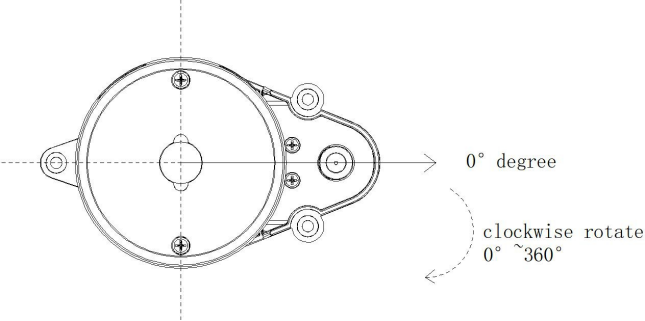
\includegraphics[width=0.7\textwidth]{orientacion_lidar.jpg}
	\caption{Orientación del sensor \cite{youyeetoo_tech_ld20_nodate}.}
	\label{fig:orientación}
\end{figure}

\subsection{Protocolo de comunicación}
El FHL-LD20 utiliza un puerto serial asíncrono estándar (UART) para la transmisión unidireccional de datos. La conexión se realiza a través de un conector ZH1.5T-4P de 1.25mm, que se utiliza tanto para la alimentación como para la transmisión de datos hacia un dispositivo \textit{Host}. En la Figura \ref{fig:pines} y en el Cuadro \ref{cuadro:parametrostrans} se muestra el orden de los pines de entrada y salida del sensor, y en el Cuadro \ref{cuadro:parametrostrans} se especifican los parámetros de transmisión.

\begin{figure}[H]
	\centering
	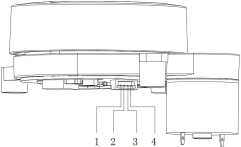
\includegraphics[width=0.4\textwidth]{pin_lidar.jpg}
	\caption{Esquema de conexión del conector ZH1.5T-4P del LiDAR FHL-LD20 \cite{youyeetoo_tech_ld20_nodate}.}
	\label{fig:pines}
\end{figure}

\begin{table}[H]
	\centering
	\resizebox{\textwidth}{!}{\begin{tabular}{|l|l|l|l|l|l|l|} 
		\hline
		\multirow{2}{*}{\centering\textbf{No. Pin}}&\multirow{2}{*}{\centering\textbf{Señal}}&\multirow{2}{*}{\centering\textbf{Tipo}}&\multirow{2}{*}{\centering\textbf{Descripción}}&\multicolumn{3}{|c|}{\textbf{Voltajes de operación}}\\
		&&&&\multicolumn{1}{|c|}{\textbf{Mínimo}}&\multicolumn{1}{|c|}{\textbf{Típico}}&\multicolumn{1}{|c|}{\textbf{Máximo}}\\
		\hline
		\multicolumn{1}{|c|}{\textbf{1}}&RX/PWM&Entrada&Control de velocidad externo&3 V&3.3 V&3.6 V\\
		\hline
		\multicolumn{1}{|c|}{\textbf{2}}&GND&Alimentación&Tierra&-&0 V&-\\
		\hline
		\multicolumn{1}{|c|}{\textbf{3}}&TZ&Salida&Salida de datos del LiDAR&3 V&3.3 V&3.6 V\\
		\hline
		\multicolumn{1}{|c|}{\textbf{4}}&VCC&Alimentación&Alimentación positiva&4.5 V&5 V&5.5 V\\
		\hline
	\end{tabular}}
	\caption{Parámetros de conexión del Lidar FHL-LD20.} 
	\label{cuadro:parametrospin}
\end{table}

\begin{table}[H]
	\centering
	\resizebox{\textwidth}{!}{\begin{tabular}{|l|l|l|l|l|} 
		\hline
		\multicolumn{1}{|c|}{\textbf{Velocidad en baudios}}&\multicolumn{1}{|c|}{\textbf{Longitud de los datos}}&\multicolumn{1}{|c|}{\textbf{Bits de parada}}&\multicolumn{1}{|c|}{\textbf{Bit de paridad}}&\multicolumn{1}{|c|}{\textbf{Control de flujo}}\\
		\hline
		230400&8 bits&1&N/A&N/A\\
		\hline
	\end{tabular}}
	\caption{Parámetros de transmisión UART.} 
	\label{cuadro:parametrostrans}
\end{table}

\subsubsection{Formato de paquete}
Cuando el sensor alcanza un estado de operación estable, comienza a enviar automáticamente paquetes de datos de medición sin requerir ninguna instrucción. En el Cuadro \ref{cuadro:paquete} se detalla la estructura general de estos paquetes de medición y el significado de cada campo.
\begin{table}[H]
	\centering
	\resizebox{\textwidth}{!}{\begin{tabular}{|l|l|l|l|l|l|l|l|l|l|l|l|} 
			\hline
			\multicolumn{1}{|c|}{\textbf{\makecell{Carácter\\de inicio}}}&\multicolumn{1}{|c|}{\textbf{VerLen}}&\multicolumn{2}{|c|}{\textbf{\makecell{Velocidad\\del radar}}}&\multicolumn{2}{|c|}{\textbf{\makecell{Ángulo\\de inicio}}}&\multicolumn{1}{|c|}{\textbf{Data}}&\multicolumn{2}{|c|}{\textbf{\makecell{Ángulo\\final}}}&\multicolumn{2}{|c|}{\textbf{\makecell{Marca\\de tiempo}}}&\multicolumn{1}{|c|}{\textbf{\makecell{Verificación\\CRC}}}\\
			\hline
			54H&2CH&LSB&MSB&LSB&MSB&...&LSB&MSB&LSB&MSB&1 Byte\\
			\hline
			\multicolumn{12}{c}{\textbf{}}\\
			\multicolumn{6}{c}{\textbf{}}&\multicolumn{1}{c}{\textbf{$\Downarrow$}}&\multicolumn{5}{c}{\textbf{}}\\
			\multicolumn{12}{c}{\textbf{}}\\
			\hline
			\multicolumn{3}{|c|}{\textbf{Punto de medición 1}}&\multicolumn{3}{|c|}{\textbf{Punto de medición 2}}&\multicolumn{3}{|c|}{\textbf{...}}&\multicolumn{3}{|c|}{\textbf{Punto de medición 12}}\\
			\hline
			\multicolumn{2}{|c|}{\textbf{Valor distancia 1}}&\textbf{Intensidad}&\multicolumn{2}{|c|}{\textbf{Valor distancia 2}}&\textbf{Intensidad}&\multicolumn{3}{|c|}{\textbf{...}}&\multicolumn{2}{|c|}{\textbf{Valor distancia 12}}&\textbf{Intensidad}\\
			\hline
			LSB&MSB&1 Byte&LSB&MSB&1 Byte&\multicolumn{3}{|c|}{\textbf{...}}&LSB&MSB&1 Byte\\
			\hline
	\end{tabular}}
	\caption{Estructura de un paquete de medición.} 
	\label{cuadro:paquete}
\end{table}

\begin{itemize}
	\item  Carácter de inicio (1 byte): Valor fijo de 0x54, señala el inicio de un paquete.
	\item  VerLen (1 byte): Valor fijo de 0x2C, especifica que cada paquete contiene 12 puntos de medición.
	\item  Velocidad del radar (2 bytes): Representa la velocidad del radar en grados por segundo.
	\item  Ángulo de inicio (2 bytes): Indica el ángulo de inicio en unidades de 0.01 grados.
	\item  Data (36 bytes): Contiene la información de 12 puntos de medición, cada uno de 3 bytes. Los primeros 2 bytes de cada punto indican el valor de distancia en milímetros, y el tercer byte refleja la intensidad de la señal de reflexión; los valores más altos indican una mayor intensidad.
	\item  Ángulo final (2 bytes): Señala el ángulo de finalización de la medición, en unidades de 0.01 grados.
	\item  Marca de tiempo (2 bytes): Representa el tiempo en milisegundos en el que se capturaron los datos.
	\item  Verificación CRC (1 byte):  Byte utilizado como \textit{checksum} para asegurar la integridad de todos los datos anteriores que forman un phaquete.
\end{itemize}

\section{Lectura de datos}
La integración de microcontroladores y software de análisis es fundamental para el desarrollo de sistemas de captura y procesamiento de datos en aplicaciones de sensores. En esta sección, se describe el proceso de lectura y decodificación de datos del sensor FHL-LD20, utilizando un microcontrolador ESP32 y plataformas de software como Matlab y Python. También, se presenta la aplicación desarrollada para la recolección e interpretación de datos del sensor, proporcionando una herramienta útil para evaluar su precisión y confiabilidad en diversos escenarios.

\subsection{Lectura e interpretación de datos mediante ESP32 y Matlab}
Para desarrollar el prototipo inicial de un sistema de captura y análisis de datos del sensor FHL-LD20, se utilizó un microncontrolador ESP32, programado mediante la plataforma de Arduino, en combinación con el software Matlab. El microcontrolador ESP32 se encargó de la recolección de información a través de la conexión UART proporcionada por el sensor. Este primer modelo permitió realizar una evaluación preliminar del rendimiento del sensor. En la Figura \ref{fig:diagrama_captura} se muestra el proceso general de captura de datos en términos generales.

\begin{figure}[H]
	\centering
	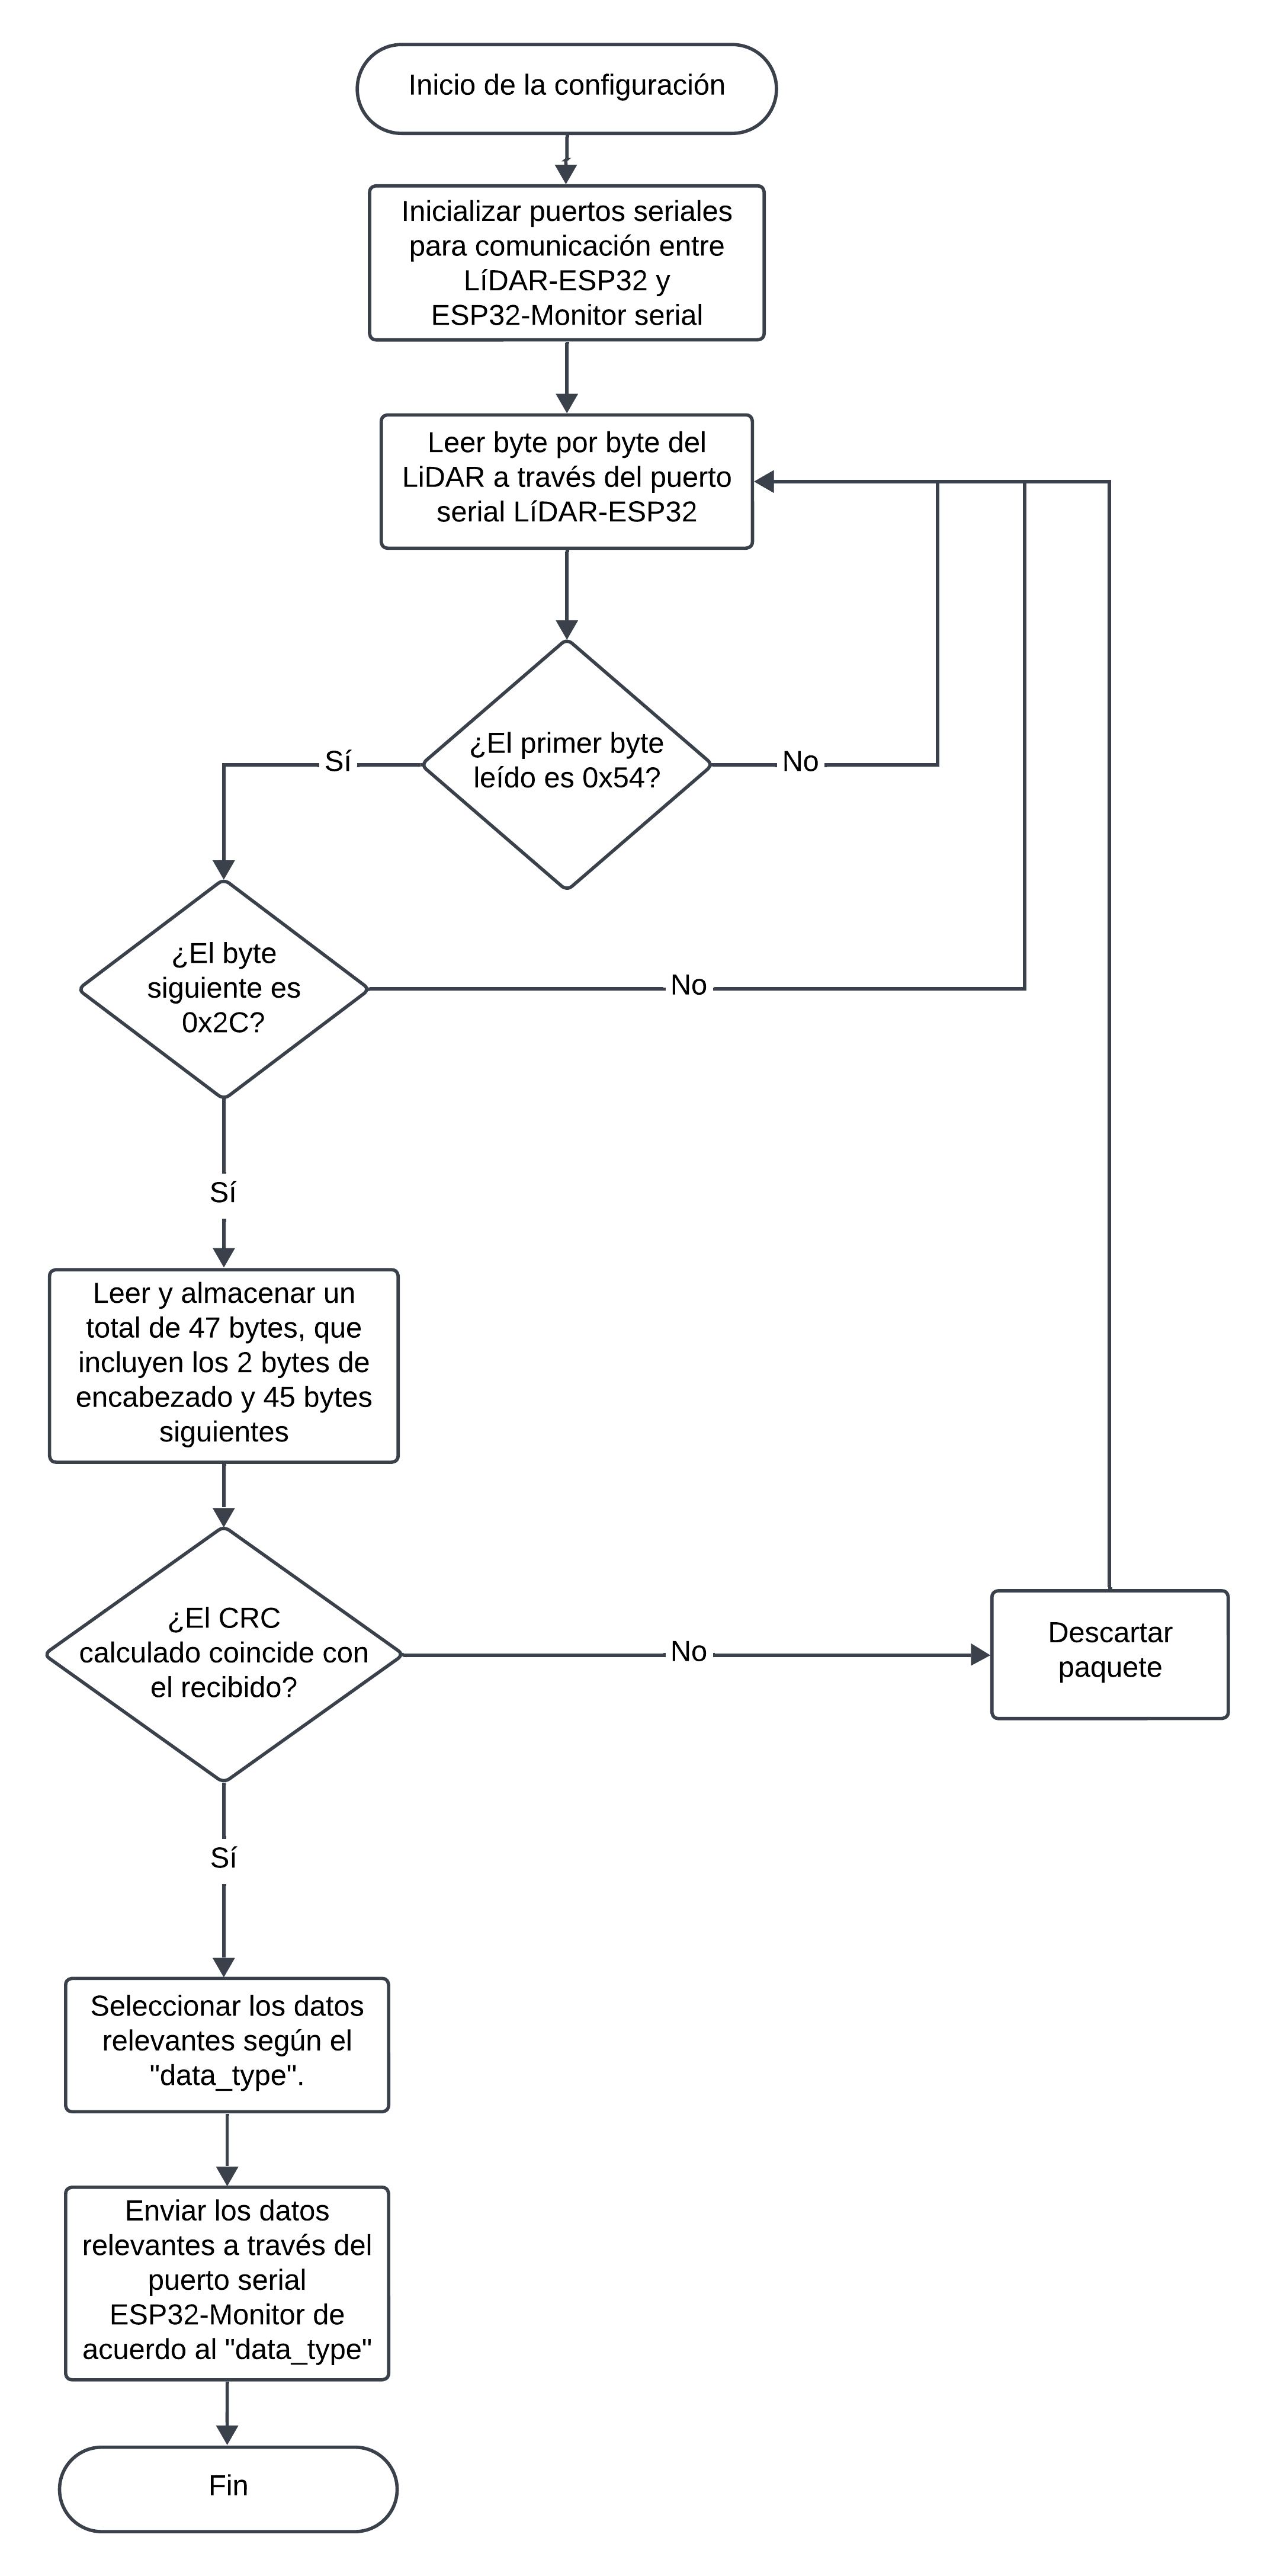
\includegraphics[width=0.6\textwidth]{diagrama_captura.png}
	\caption{Diagrama de flujo general para captura de datos provenientes del sensor.}
	\label{fig:diagrama_captura}
\end{figure}

El proceso de captura de datos sigue una estructura de validación en la que se espera recibir un paquete de 47 bytes. Cada paquete se valida mediante los dos bytes de encabezados específicos (0x54 y 0x2C), una vez recibido el paquete completo, se realiza una verificación de integridad utilizando un cálculo de verificación por redundancia cíclica (CRC) de 8 bits. El código opera de manera cíclica en el bucle principal, lo que permite un flujo continuo de lectura de datos del LiDAR. 

En el diagrama de flujo presentado se destaca la importancia de la variable ``data\_type''. Esta variable define la cantidad de datos que el microcontrolador enviará a Matlab para su procesamiento. Dicha variable puede asumir uno de tres valores predefinidos: ``FULL\_DATA'', ``RELEVANT\_DATA'' o ``RELEVANT\_DATA2'', cada uno especificando una longitud distinta para los datos a transmitir.
\begin{itemize}
	\item  ``FULL\_DATA'': Corresponde a un paquete completo de 47 bytes (94 caracteres).
	\item ``RELEVANT\_DATA'': Paquete de 30 bytes que excluye la velocidad del radar, los bytes de intensidad de la señal, los de la marca de tiempo y el byte de verificación CRC (60 caracteres).
	\item ``RELEVANT\_DATA2'': Paquete de 42 bytes que, a diferencia de ``RELEVANT\_DATA'', incluye los bytes de intensidad de la señal (84 caracteres).
\end{itemize}
La flexibilidad en el tamaño de los paquetes fue implementada para optimizar el tiempo de procesamiento en Matlab, lo cual es particularmente relevante en aplicaciones en tiempo real o cuando se manejan múltiples paquetes de datos en rápida sucesión. Al reducir la cantidad de información procesada, se logra una respuesta más rápida del sistema sin necesidad de realizar cambios significativos en el software. Cabe destacar que los datos capturados se envían como una cadena de caracteres hexadecimales a través del puerto serial.

Una vez capturada la información del sensor, se utilizó Matlab para desarrollar un programa capaz de recibir los datos transmitidos desde el microcontrolador. El software permitió obtener y decodificar múltiples lecturas consecutivas, así como graficar los resultados. Este proceso se utilizó para verificar la concordancia de las lecturas del sensor con los valores esperados, además de ofrecer una herramienta sencilla para manipular los datos recibidos. La Figura \ref{fig:diagrama_procesamiento} muestra el proceso de recepción, decodificación y visualización de los datos obtenidos.

\begin{figure}[H]
	\centering
	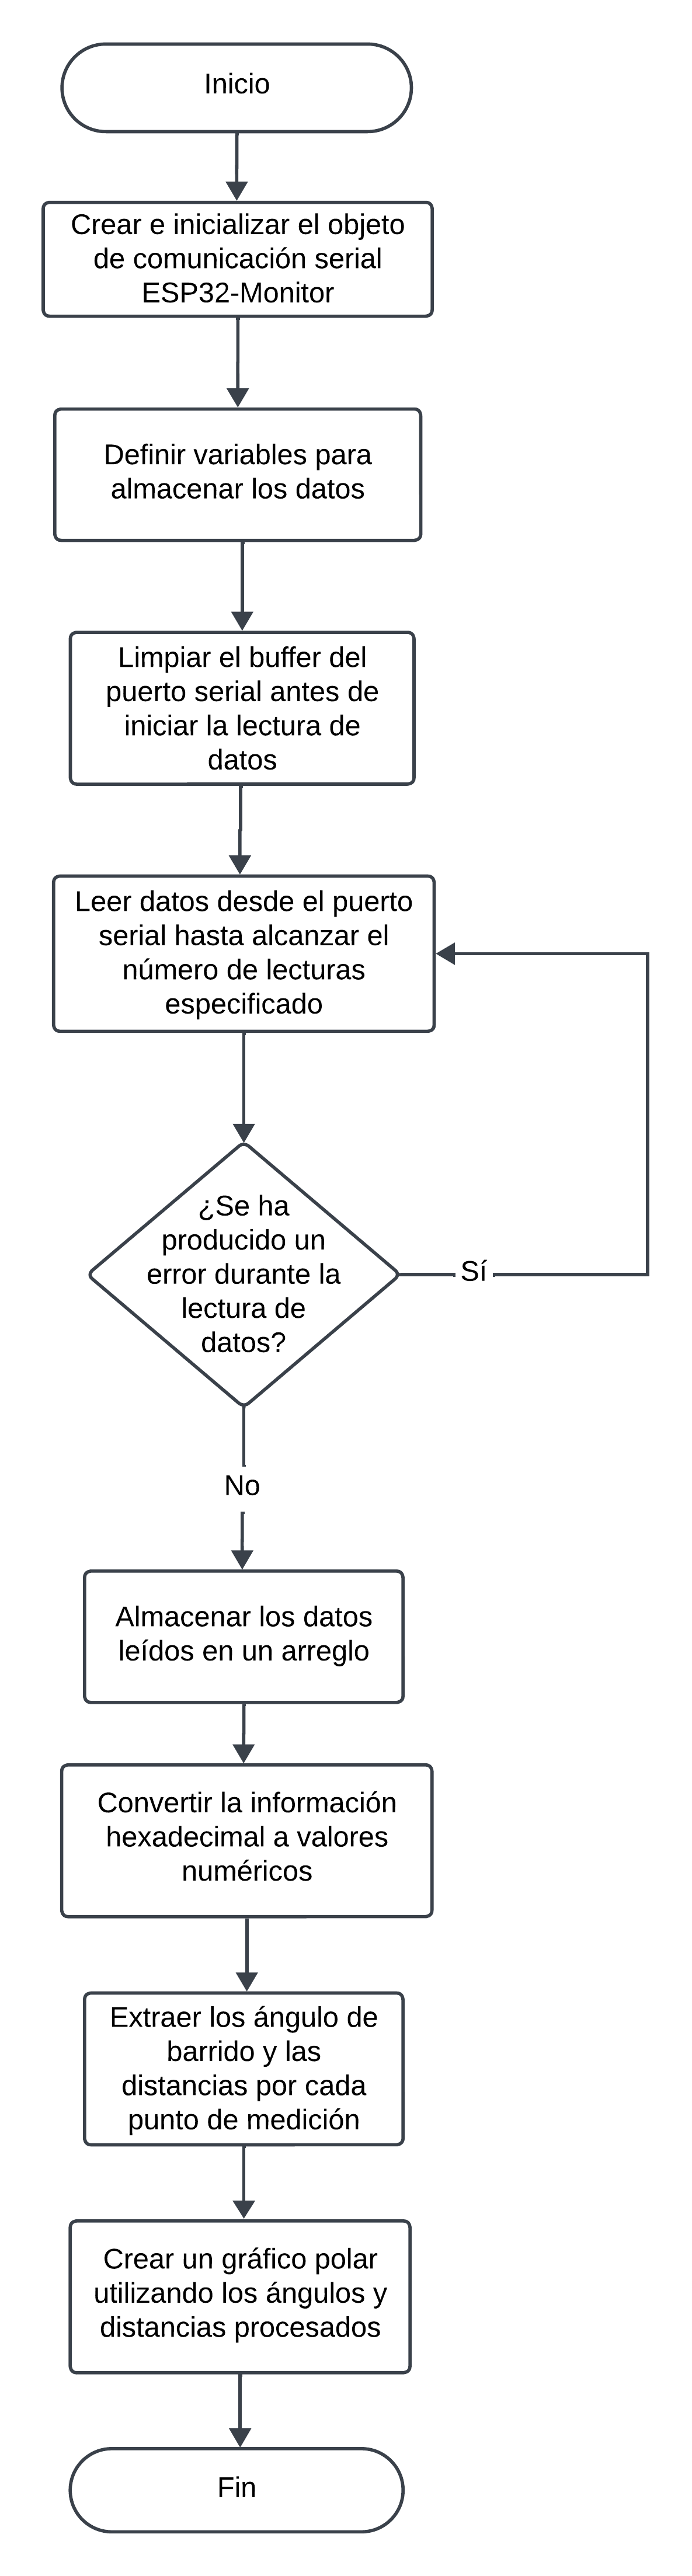
\includegraphics[width=0.33\textwidth]{diagrama_procesamiento.png}
	\caption{Diagrama de flujo general para procesamiento de datos provenientes del sensor.}
	\label{fig:diagrama_procesamiento}
\end{figure}

Como se mencionó anteriormente, el paquete de datos recibido consiste en un arreglo de caracteres que contiene información estructurada en formato hexadecimal. La conversión de datos se realiza dividiendo el paquete en segmentos y extrayendo pares de caracteres hexadecimales. Para reconstruir los valores completos de ángulos y distancias, se combinan dos partes: un byte de menor orden y un byte de mayor orden. 

Por ejemplo, para el ángulo de inicio codificado en dos bytes, se extraen las partes de menor y mayor orden para obtener los valores hexadecimales correspondientes. Luego, se desplaza el byte de mayor orden a la posición correcta dentro del valor de 16 bits y se suma con el byte de menor orden para obtener el valor completo. De esta manera, se reconstruye el valor decimal correspondiente al ángulo de inicio medido, expresado en unidades de 0.01 grados, en el paquete de datos evaluado como se muestra en la Figura \ref{fig:data_in}.

\begin{figure}[H]
	\centering
	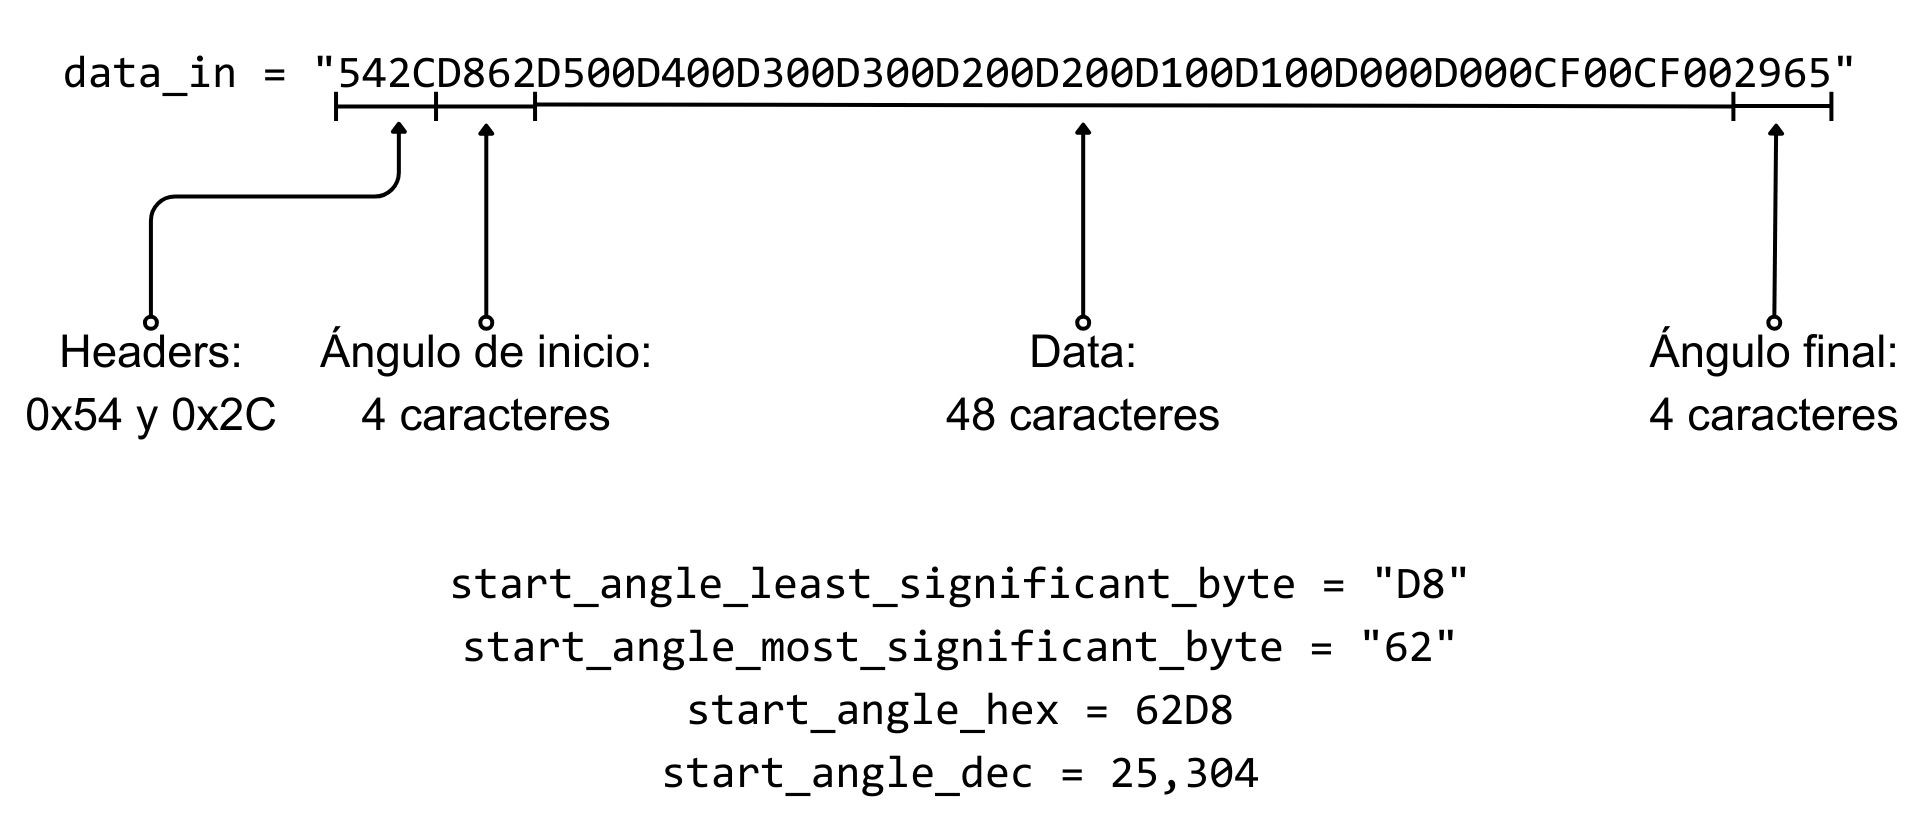
\includegraphics[width=0.8\textwidth]{data_in.jpg}
	\caption{Ejemplificación del proceso de reconstrucción de mediciones: ángulo de inicio.}
	\label{fig:data_in}
\end{figure}

Una vez que las lecturas fueron decodificadas y segmentadas en sus partes correspondientes, se calculó el ángulo de barrido para cada punto de distancia. Este cálculo se realizó determinando el paso angular, el cual fue obtenido al dividir la diferencia entre los ángulos de inicio y fin por el número de intervalos entre los puntos de medición. Este incremento angular fue sumado acumulativamente al angulo de inicio. De esta manera, a cada punto de distancia medido se le asignaría un ángulo de barrido específico. Cabe destacar que la diferencia entre los ángulos de inicio y fin fue de aproximadamente 6°, lo que implica que cada paquete de datos cubre un barrido de esta magnitud.

Los valores de distancias y ángulos resultantes del procesamiento de datos se organizaron en una matriz de datos la cual se representó en una gráfica de coordenadas polares en Matlab para recrear la visualización generada por el LiDAR. Para verificar su funcionamiento y realizar un reconocimiento de área, se colocó el sensor FHL-LD20 dentro de una caja de 38.5$\times$23 cm. En la Figura \ref{primera_corrida} se presenta la disposición del sensor dentro de la caja y la reconstrucción visual realizada a partir de 60 paquetes del puerto serial, es decir, 720 puntos de medición procesados o bien, una revolución completa.

\begin{figure}[H]
	\centering
	\begin{subfigure}{0.8\textwidth}
		\centering
		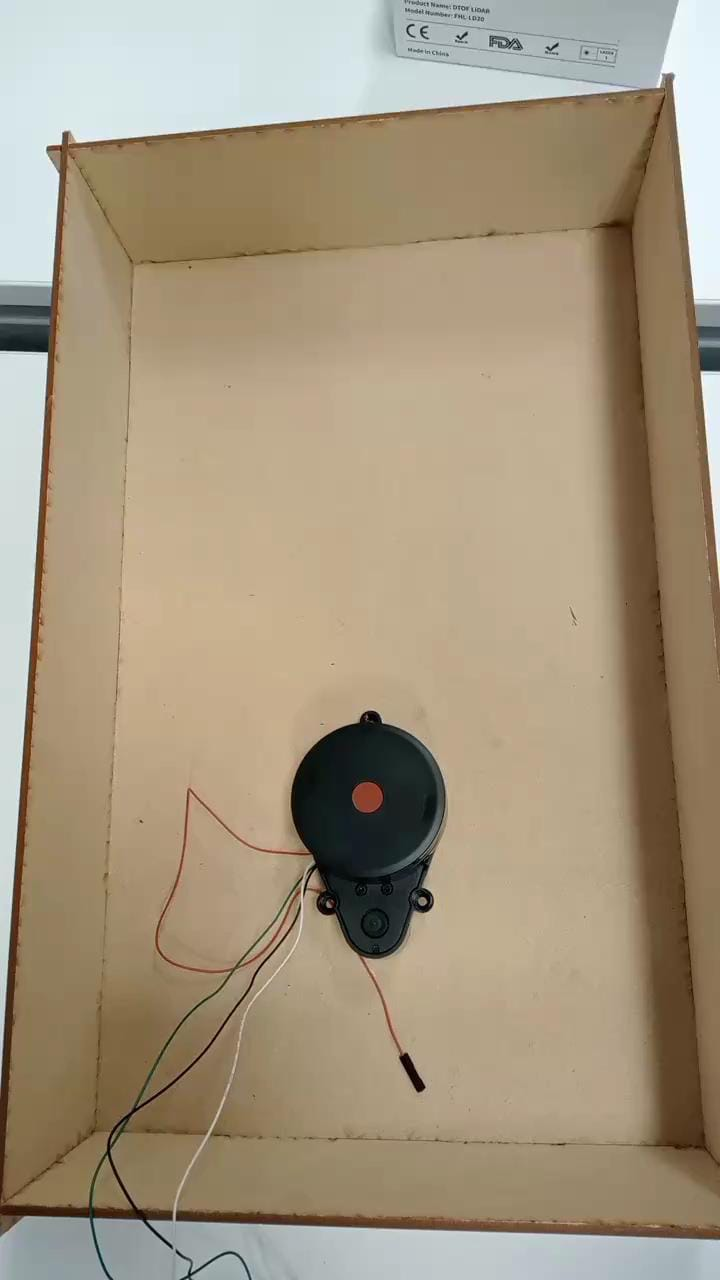
\includegraphics[angle=270,width=0.8\linewidth]{disposicion_lidar1.jpeg}
		\caption{Disposición del sensor FHL-LD20 dentro de la caja.}
		\label{primera_corrida_disp}
		\vspace{1em}
	\end{subfigure}
	\begin{subfigure}{0.8\textwidth}
		\centering
		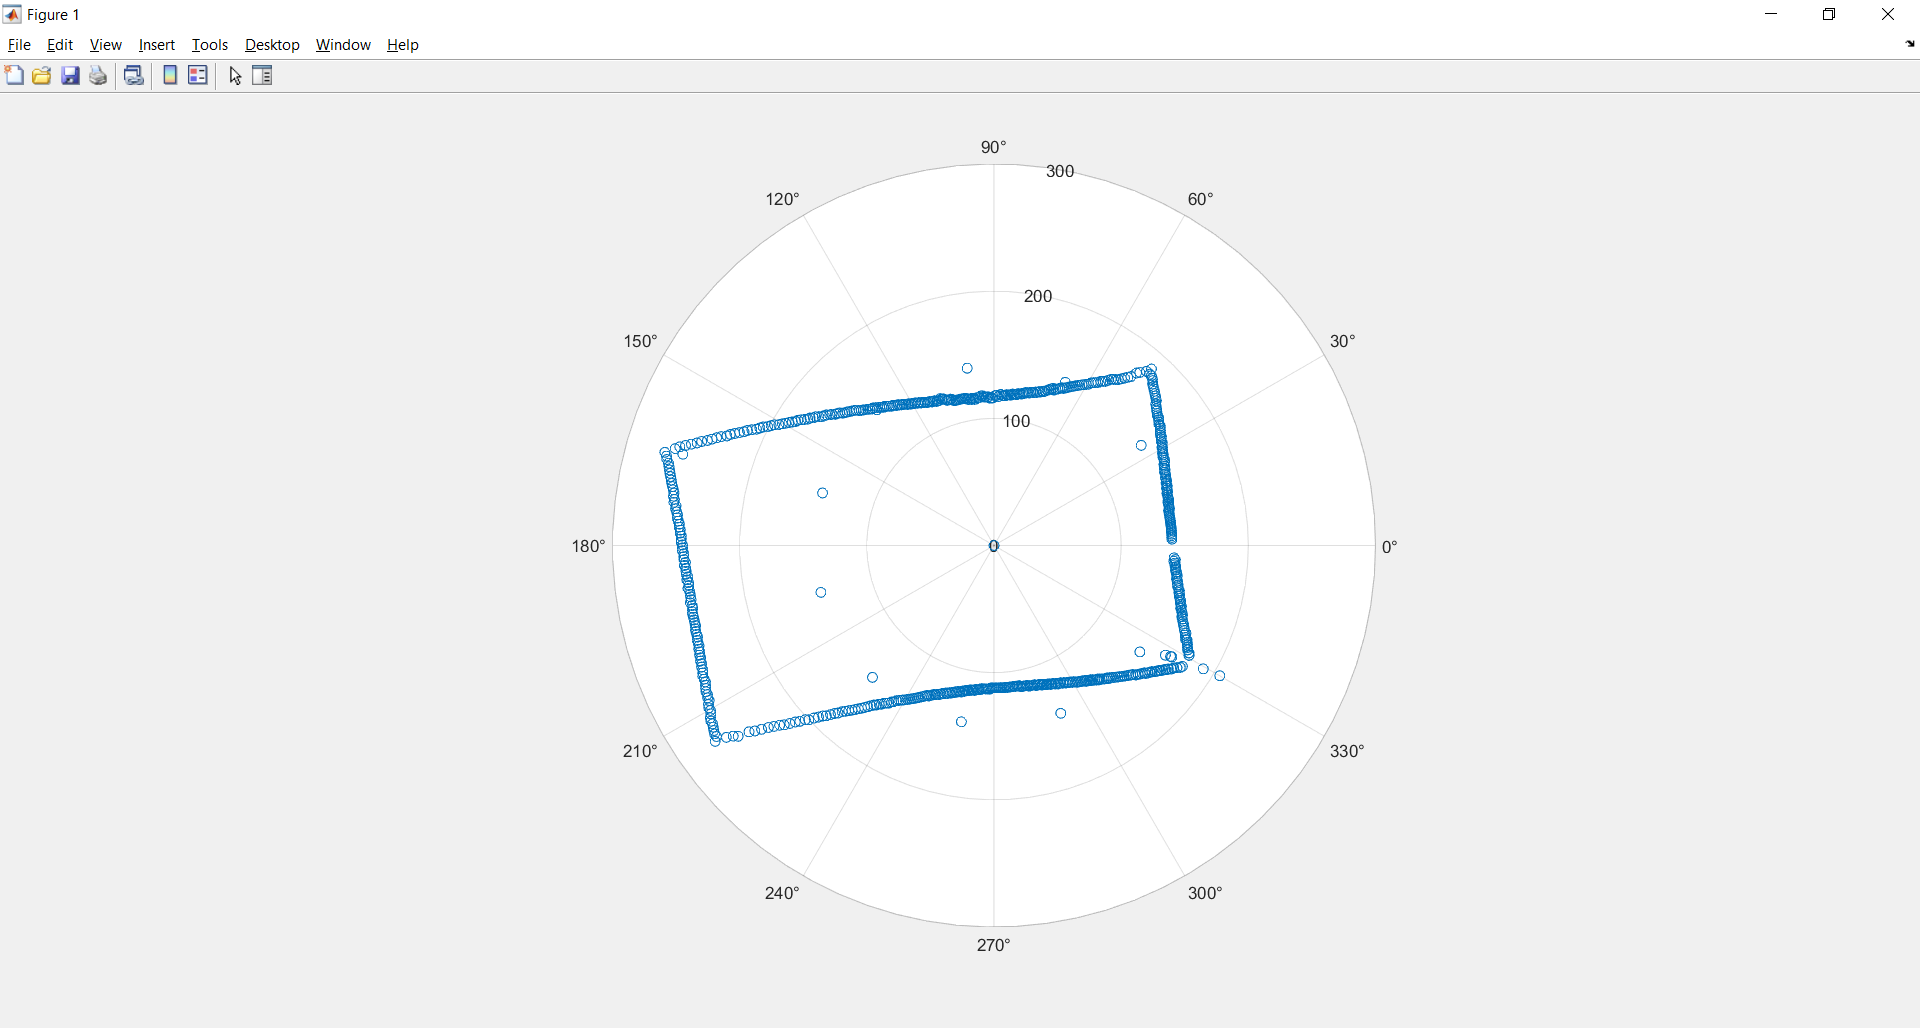
\includegraphics[width=0.8\linewidth]{primera_lectura.png}
		\caption{Reconstrucción de las 70 lecturas del sensor.}
		\label{primera_corrida_recon}
	\end{subfigure}
	\caption{Visualización de la primera corrida del sensor: 840 puntos de medición.}
	\label{primera_corrida}
\end{figure}
A partir de la Figura \ref{primera_corrida_recon}, se identificaron distintas áreas de mejora al momento de realizar la reconstrucción. En primer lugar, aunque la forma y las proporciones generales de la caja se representaron correctamente, la reconstrucción se presenta de manera ``invertida'' en comparación con la disposición física observada (Figura \ref{primera_corrida_disp}). La causa de esta discrepancia radica en que el LiDAR captura los datos en dirección horaria, mientras que los sistemas de visualización convencionales suelen interpretar los datos en sentido antihorario. Como resultado, la orientación visual de la reconstrucción difiere con lo que se observa a simple vista. Este hecho resaltó la necesidad de implementar una opción para ajustar la orientación de los puntos capturados, de modo que la reconstrucción se alinee con la disposición física y sea más intuitiva.

Otro aspecto destacable es la ligera curvatura observada en las aristas de la reconstrucción, que difiere con los bordes rectos de la caja física. Esta distorsión surgió debido a que los datos se procesaron sin considerar el ajuste para alinear los puntos obtenidos con el sistema de referencia deseado (eje central de rotación del sensor como origen). Es decir, no se aplicó una compensación adecuada para corregir los desfases entre el sistema de coordenadas en el que se capturan las mediciones (propio del LiDAR) y el sistema de coordenadas en el que se deberían de visualizar los datos (eje central). Como resultado, la reconstrucción presenta una leve deformación en comparación con la realidad física observada.

Además, se identificó un conjunto de aproximadamente 10 puntos distribuidos de forma circular que no deberían de estar presentes en la reconstrucción. Al revisar el procesamiento de datos, se determinó que estos puntos atípicos surgieron debido a un error en el cálculo del barrido angular. Cuando el ángulo de inicio era mayor que el ángulo final, se obtenía una diferencia negativa, lo que provocaba que las mediciones cercanas al cruce del punto de 0 grados se distorsionaran. Para solventar esto, se implementó una corrección en el cálculo del ángulo, añadiendo 360 grados cuando el ángulo de inicio superaba al ángulo final. Esta corrección garantizaba una transición continua entre mediciones al momento en que el sensor completaba un ciclo y cruzaba por el ángulo de 0 grados. Estos detalles no solo resaltaron la importancia de revisar cuidadosamente el procesamiento de datos, sino también la necesidad de diseñar un soporte para estabilizar y alinear adecuadamente el sensor LiDAR.

\subsection{Lectura e interpretación de datos mediante ESP32 y Python}
En lugar de desarrollar únicamente un software para obtener y procesar los datos, se decidió crear una aplicación que mejorara la experiencia del usuario al utilizar el sensor FHL-LD20. Para ello, se optó por utilizar Python 3.11 como lenguaje de programación, considerando la necesidad de un entorno más flexible y eficiente para el manejo de datos. Las principales razones por las cuales se seleccionó Python sobre Matlab, que se había usado anteriormente, fueron las siguientes:
\begin{itemize}
	\item  A diferencia de Matlab, Python es un lenguaje de código abierto y gratuito. 
	\item Python cuenta con un ecosistema amplio, con una gran variedad de librerías y \textit{frameworks} que facilitan la integración de diferentes funcionalidades en una misma aplicación.
	\item Para el desarrollo de aplicaciones de escritorio, Python ofrece múltiples frameworks como Tkinter, PyQT y Kivy, mientras que Matlab sólo dispone de App Designer para la creación de interfaces gráficas.
	\item Python cuenta con una comunidad de desarrolladores muy grande y activa, lo que facilita la resolución de problemas y la implementación de nuevas funcionalidades.
\end{itemize}
Cabe señalar que el código desarrollado para el ESP32, se mantuvo sin cambios, ya que mostró ser eficiente para la recolección de datos.

Ahora bien, para el desarrollo de la aplicación, se empleó CustomTkinter, una extensión moderna y estilizada de Tkinter. Esta elección no solo permitió mejorar la estética de la interfaz, sino que también ofreció una experiencia más funcional en comparación con herramientas tradicionales, como Tkinter. En la Figura \ref{fig:vista_interfaz}, se presenta la interfaz gráfica nombrada ``LiDAR MapViewer'', junto con las distintas opciones y paneles disponibles dentro de la aplicación. Es importante destacar que el procesamiento de datos siguió la misma estructura general que el diagrama de flujo presentado en la Figura \ref{fig:diagrama_procesamiento}. Las modificaciones específicas realizadas se detallan en el siguiente capítulo.

\begin{figure}[H]
	\centering
	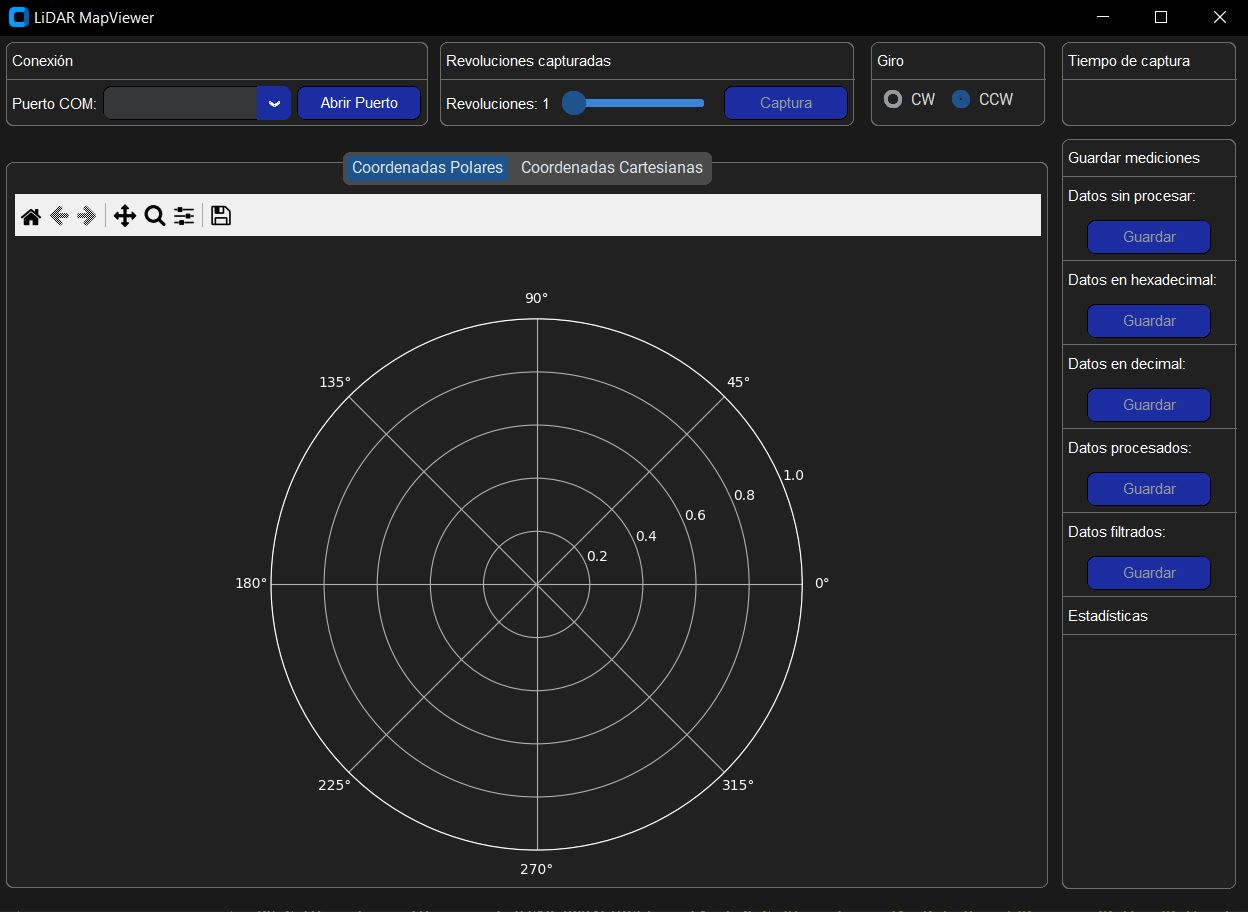
\includegraphics[width=0.9\textwidth]{app.jpg}
	\caption{Vista de usuario, interfaz gráfica LiDAR MapViewer.}
	\label{fig:vista_interfaz}
\end{figure}

\begin{itemize}
	\item  Panel de conexión: Este panel gestiona la conexión entre el ESP32 y el monitor a través de un puerto serial, que puede seleccionarse mediante un menú desplegable que muestra los puertos COM disponibles. La conexión se habilita mediante un botón, siempre que el puerto COM se encuentra activo y disponible. 
	\item Panel de revoluciones capturadas: Este marco contiene los controles para seleccionar y visualizar el número de revoluciones capturadas por el LiDAR. Incluye un control deslizante que permite elegir entre 1 y 5 revoluciones, y un botón para iniciar la captura de datos.
	\item Panel de giro: Este panel cuenta con dos botones que permiten al usuario seleccionar la orientación del giro  de los datos capturados por el LiDAR. Este selección ajusta el cálculo de los ángulos para su visualización.
	\item Panel de tiempo de captura: Muestra el tiempo total empleado por la interfaz para capturar, procesar y graficar todas las muestras seleccionadas por el usuario. El panel se actualiza al finalizar el proceso de captura.
	\item Panel de gráficos: Este marco contiene los gráficos de la interfaz, donde se visualizan los resultados de los datos capturados por el LiDAR, tanto en formato polar como cartesiano.
	\item Panel de guardado de mediciones: Este panel ofrece cinco opciones para almacenar distintos conjuntos de datos en archivos CSV:
	\begin{itemize}
		\item Datos sin procesar.
		\item Datos segmentados en hexadecimal.
		\item Datos segmentados en decimal.
		\item Datos procesados de ángulos y distancias.
		\item Datos filtrados de ángulos y distancias. 
	\end{itemize}
	Cada botón permite al usuario elegir la ubicación donde se guardará la información, simplificando así la organización y el análisis de los datos recopilados.
	\item Panel de pruebas estadísticas: Sección en la cual se muestran los análisis estadísticos de las aristas capturadas por el sensor. Esta sección solamente aplica para reconstrucciones de entornos cuadriláteros.
\end{itemize}

\chapter{Caracterización del LiDAR FHL-LD20}
En este capítulo se presenta la caracterización del sensor LiDAR FHL-LD20, un proceso que permite evaluar y modelar con precisión la confiabilidad de sus mediciones en condiciones reales de operación. Este análisis tiene como objetivo estudiar las variaciones y el ruido presente en las mediciones de distancia y ángulo proporcionadas por el sensor. La caracterización permite obtener una compresión detallada de los parámetros de incertidumbre del LiDAR, lo que facilita su integración en algoritmos de percepción y navegación autónoma, como el filtro de Kalman extendido (EKF). Este proceso es fundamental para validar las especificaciones proporcionadas por el fabricante, que pueden no reflejar el rendimiento en el entorno real de uso. Además, la caracterización permite adaptar el sensor a las condiciones específicas de la aplicación, identificar limitaciones, y optimizar su configuración para maximizar su rendimiento en la implementación final.

\section{Desarrollo de plataforma física para pruebas con el LiDAR FHL-LD20}
La plataforma para pruebas preliminares se diseñó utilizando el software de Autodesk Inventor 2024. La estructura consistía en una base cuadrada de 400$\times$400 mm sobre la cual se montaban cuatro paredes de 70 mm de altura de dos clases. Como se muestra en la Figura \ref{fig:pared_ranura}, la primera clase de pared presentaba divisiones escalonadas cada 10 mm, lo que permitía sujetar otras paredes y brindar modularidad a la plataforma. Esta pared también contaba con dos ranuras: una para deslizar y ajustar su posición sobre la plataforma, y otra para facilitar el paso de los cables de conexión del sensor. La segunda, en cambio, era una pieza sin divisiones (ver Figura \ref{fig:pared_normal}), diseñada para proporcionar soporte estructural adicional y cerrar la plataforma.

\begin{figure}[H]
	\centering
	\begin{subfigure}{0.5\textwidth}
		\centering	
		
\includegraphics[width=1\linewidth]{pared_ranura.jpg}
		\caption{Pared modular con divisiones y ranuras.}
		\label{fig:pared_ranura}
	\end{subfigure}%
	\begin{subfigure}{0.5\textwidth}
		\centering
		
\includegraphics[width=1\linewidth]{pared_normal.jpg}
		\caption{Pared lisa de soporte estructural.}
		\label{fig:pared_normal}
	\end{subfigure}
	
	\caption{Vista frontal de las dos clases de paredes laterales que componen la plataforma de pruebas.}
	\label{fig:pared}
\end{figure}

En la Figura \ref{fig:base} se observa que la base de la plataforma fue cubierta con una cuadrícula milimetrada en la que se marcaron cuatro líneas diagonales a 45, 135, 225 y 315 grados. Esto se realizó con el objetivo de proporcionar referencias visuales precisas de las dimensiones de la plataforma para el montaje de las paredes y la alineación exacta del sensor en el espacio. Además, se diseñó un soporte para sujetar y nivelar el sensor, incorporando dos patrones radiales que simulaban una brújula (ver Figura \ref{fig:soporte}). Estos patrones se ubicaron a 135 y 225 grados desde el centro ideal del sensor, con un desplazamiento de 30 mm. Esta disposición permitió alinear el LiDAR correctamente, ya que, al estar su centro bloqueado visualmente, los patrones desplazados proporcionaban puntos de referencia para centrarlo con precisión, teniendo en cuenta la distancia radial de 30 mm y las diagonales de la base. 

\begin{figure}[H]
	\centering
	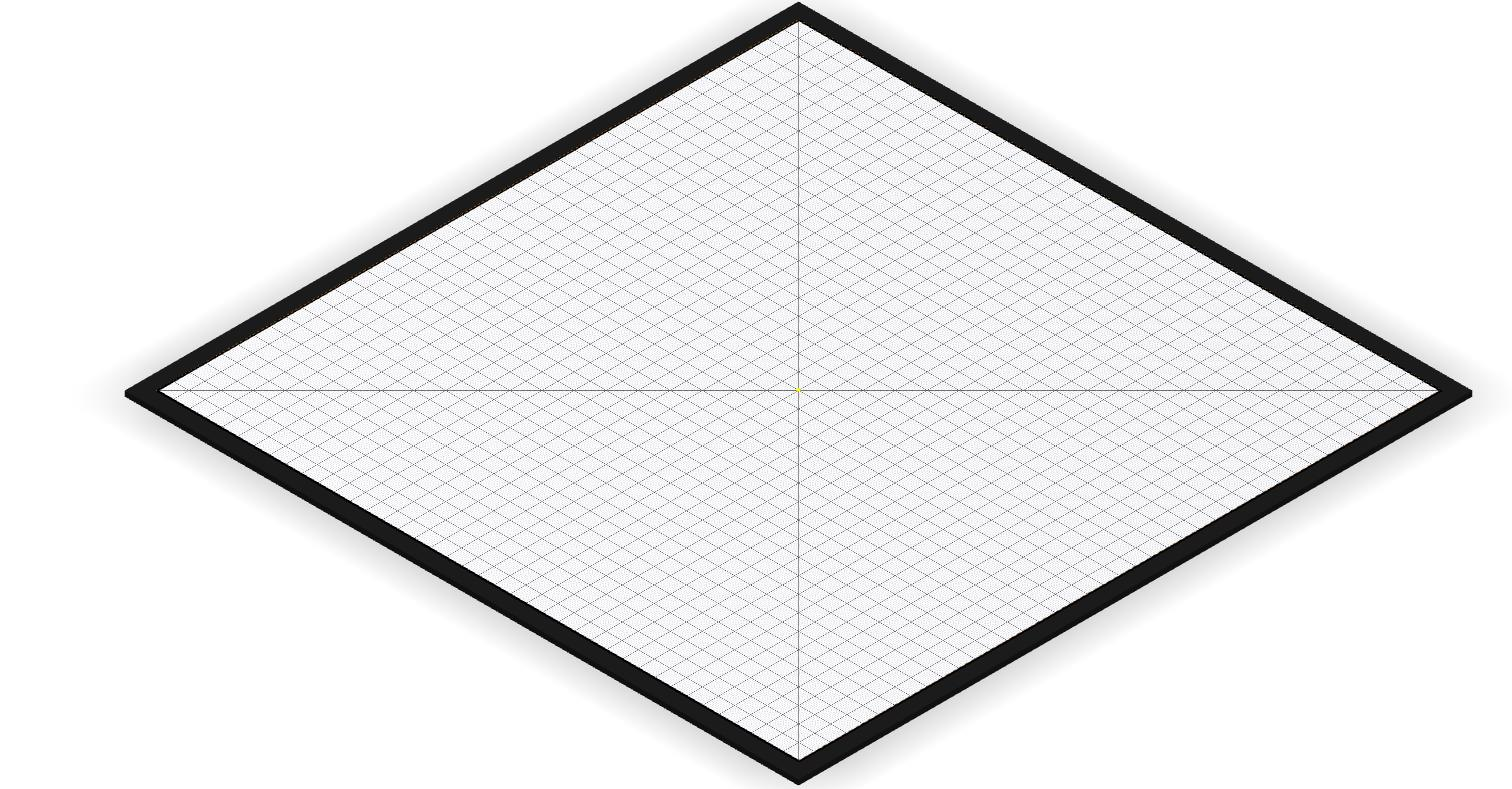
\includegraphics[width=0.6\textwidth]{base.jpg}
	\caption{Vista isométrica de la base de la plataforma de pruebas.}
	\label{fig:base}
\end{figure}

\begin{figure}[H]
	\centering
	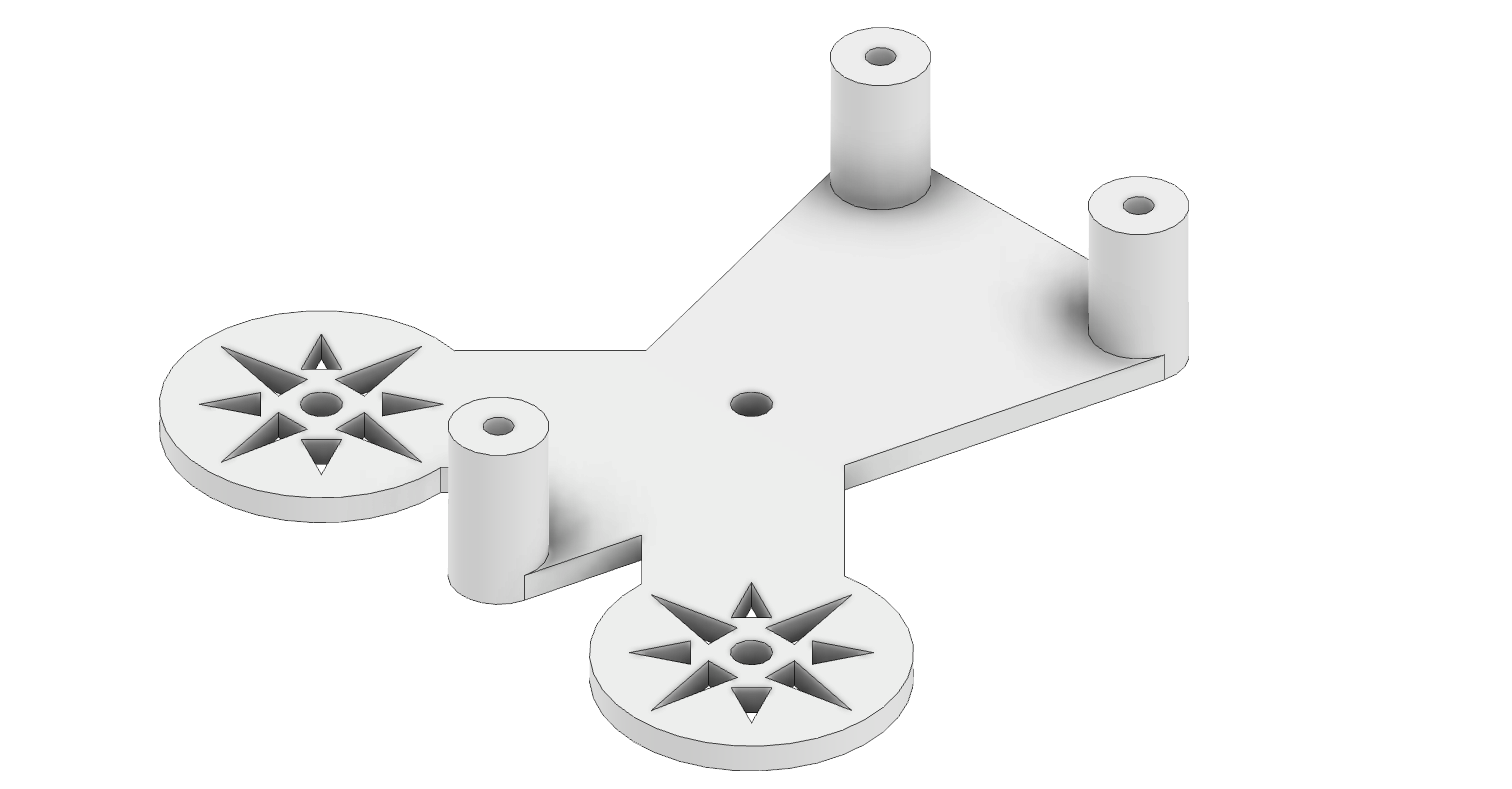
\includegraphics[width=0.5\textwidth]{base_lidar.png}
	\caption{Vista isométrica del soporte para el LiDAR FHL-LD20.}
	\label{fig:soporte}
\end{figure}

Las referencias visuales en la cuadrícula y las paredes de la plataforma permitieron comparar las lecturas obtenidas por el sensor con las dimensiones conocidas de la plataforma, ayudando a identificar cualquier desviación en las lecturas y permitiendo realizar ajustes en la orientación del sensor. Este escenario controlado aseguraba que cada medición del sensor fuera consistente y replicable en diversas pruebas. En la Figura \ref{fig:plataforma_pruebas} se presenta el diseño del ensamble final de la plataforma de pruebas, mientras que en la Figura \ref{fig:plataforma_fisica} se muestra la plataforma física fabricada junto con una reconstrucción visual del entorno, generada a partir de las lecturas del LiDAR tras el proceso de calibración descrito en la Sección \ref{sec:calibracion}.

\begin{figure}[H]
	\centering
	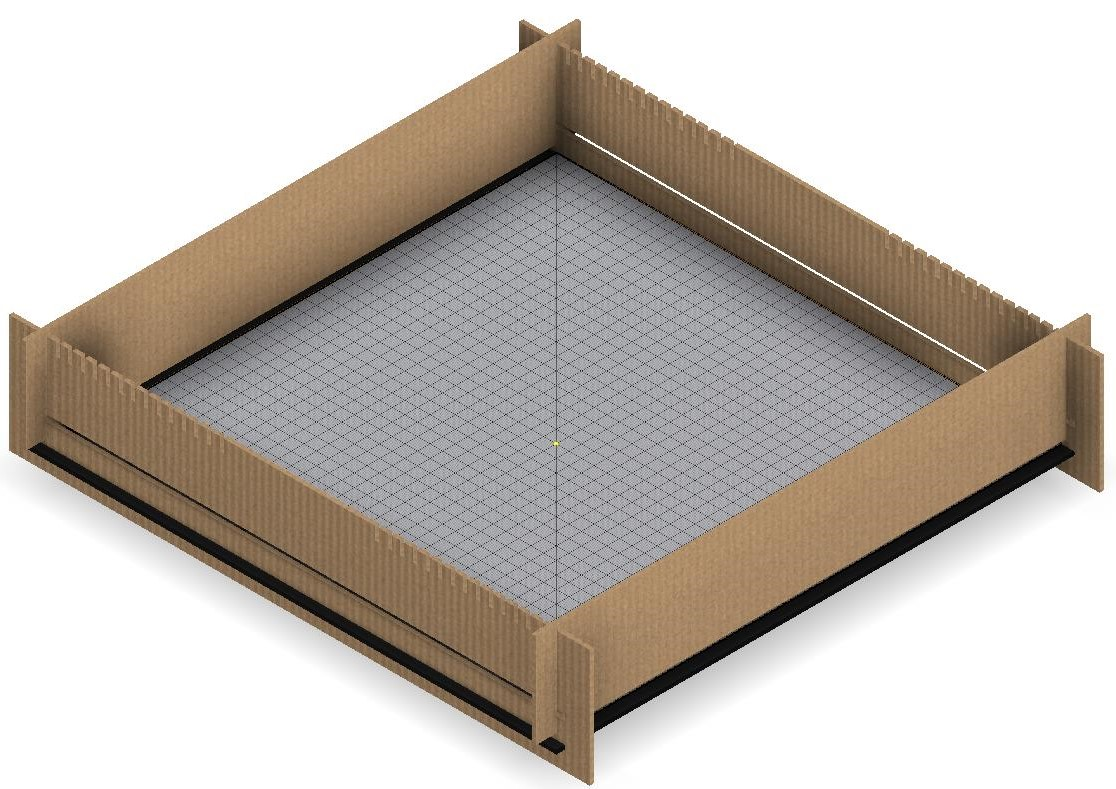
\includegraphics[width=0.6\textwidth]{plataforma_cad2.jpg}
	\caption{Vista isométrica de la plataforma de pruebas.}
	\label{fig:plataforma_pruebas}
\end{figure}

\begin{figure}[H]
	\centering
	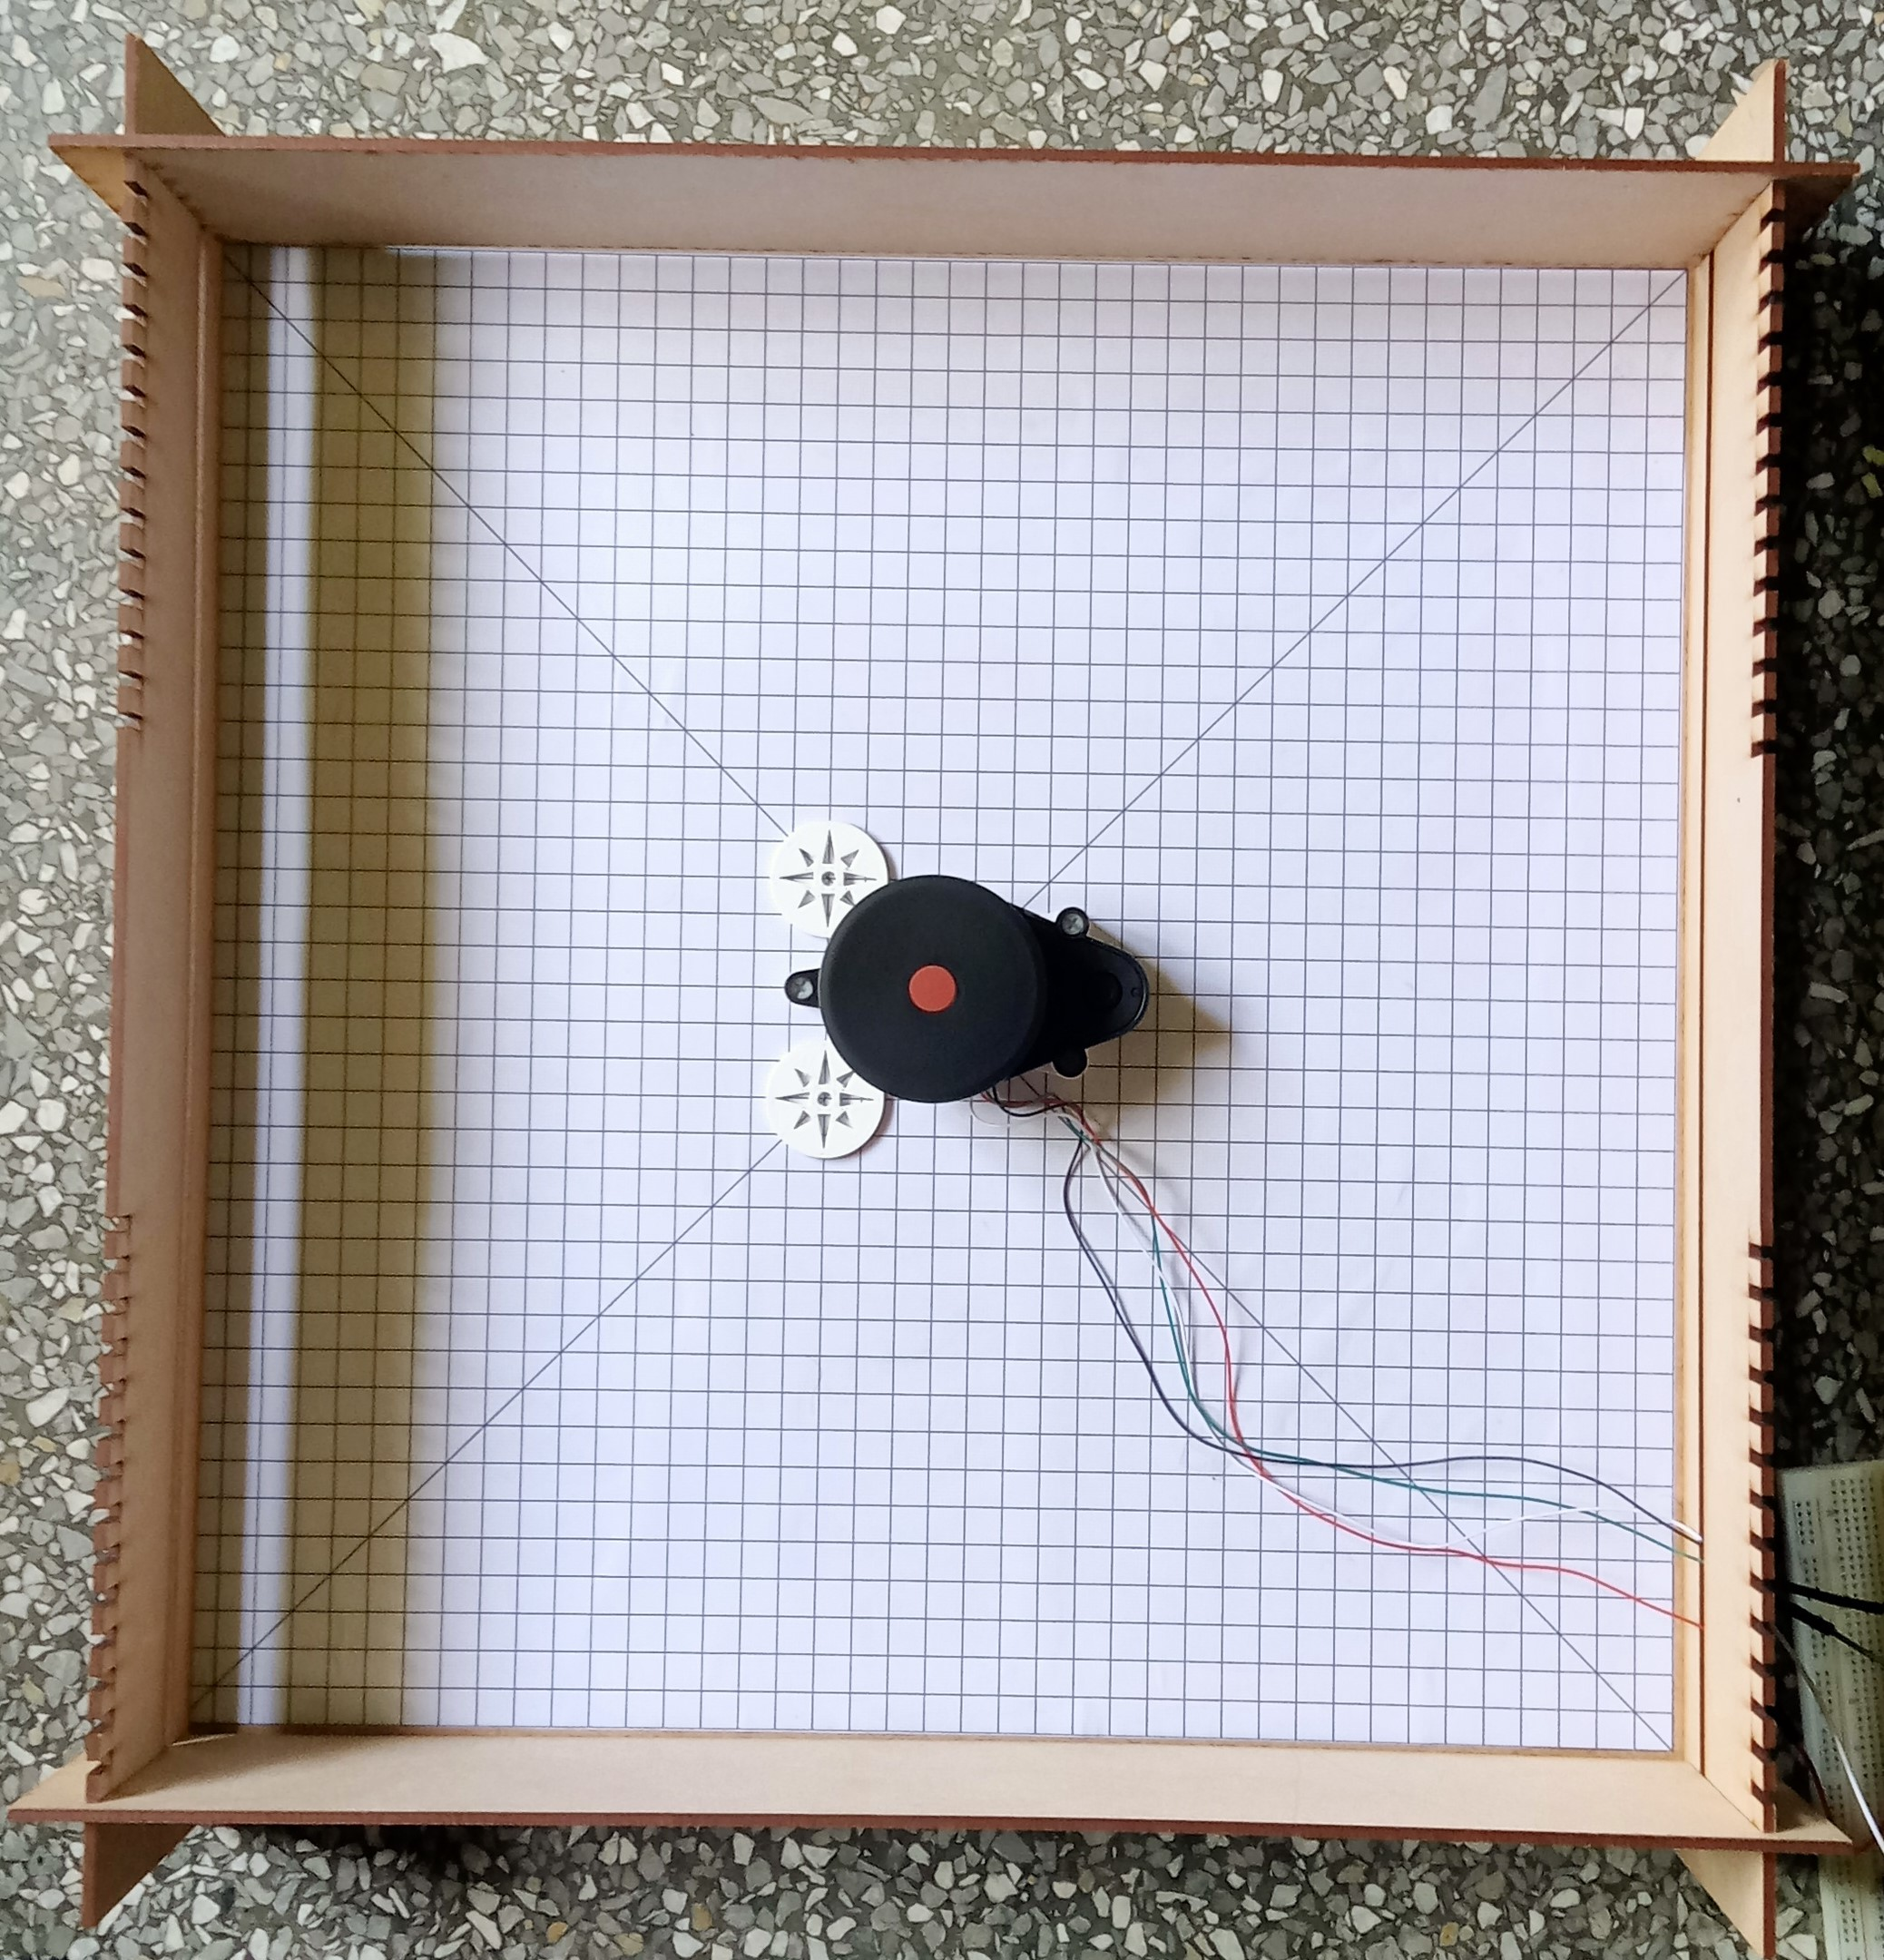
\includegraphics[width=0.5\textwidth]{plataforma.jpg}
	\caption{Vista superior de la plataforma de pruebas.}
	\label{fig:plataforma_fisica}
\end{figure}

Para asegurar una detección eficiente y minimizar el ruido generado por componentes estructurales de los agentes robóticos donde se instalará el sensor, se definió un rango mínimo de operación de 15 cm. Considerando un robot móvil como el Pololu 3pi+, permitir que el sensor opere a distancias menores podría hacer que registre elementos de su propia estructura, afectando negativamente la precisión de las mediciones. Además, dado que es poco probable encontrar obstáculos relevantes a menos de 15 cm, este límite permite enfocar la detección en elementos que realmente impacten la navegación y mejoren la maniobrabilidad del robot.

\section{Depuración de mediciones nulas en el LiDAR FHL-LD20}
Como se describe en la Sección \ref{sec:calibracion}, el proceso de calibración utiliza las distancias en formato decimal, para calcular el ángulo de corrección, el cual ajusta la posición angular de los puntos medidos por el LiDAR. En el diagrama de flujo (Figura \ref{fig:diagrama_procesamiento_dec}), se puede apreciar que el procesamiento depende de si la distancia medida es mayor a cero. Cuando es mayor, se calculan tanto los valores de ajuste como el ángulo de desplazamiento real. Una vez determinado el ángulo real, se actualiza el valor del ángulo de corrección antiguo por el más reciente.

\begin{figure}[H]
	\centering
	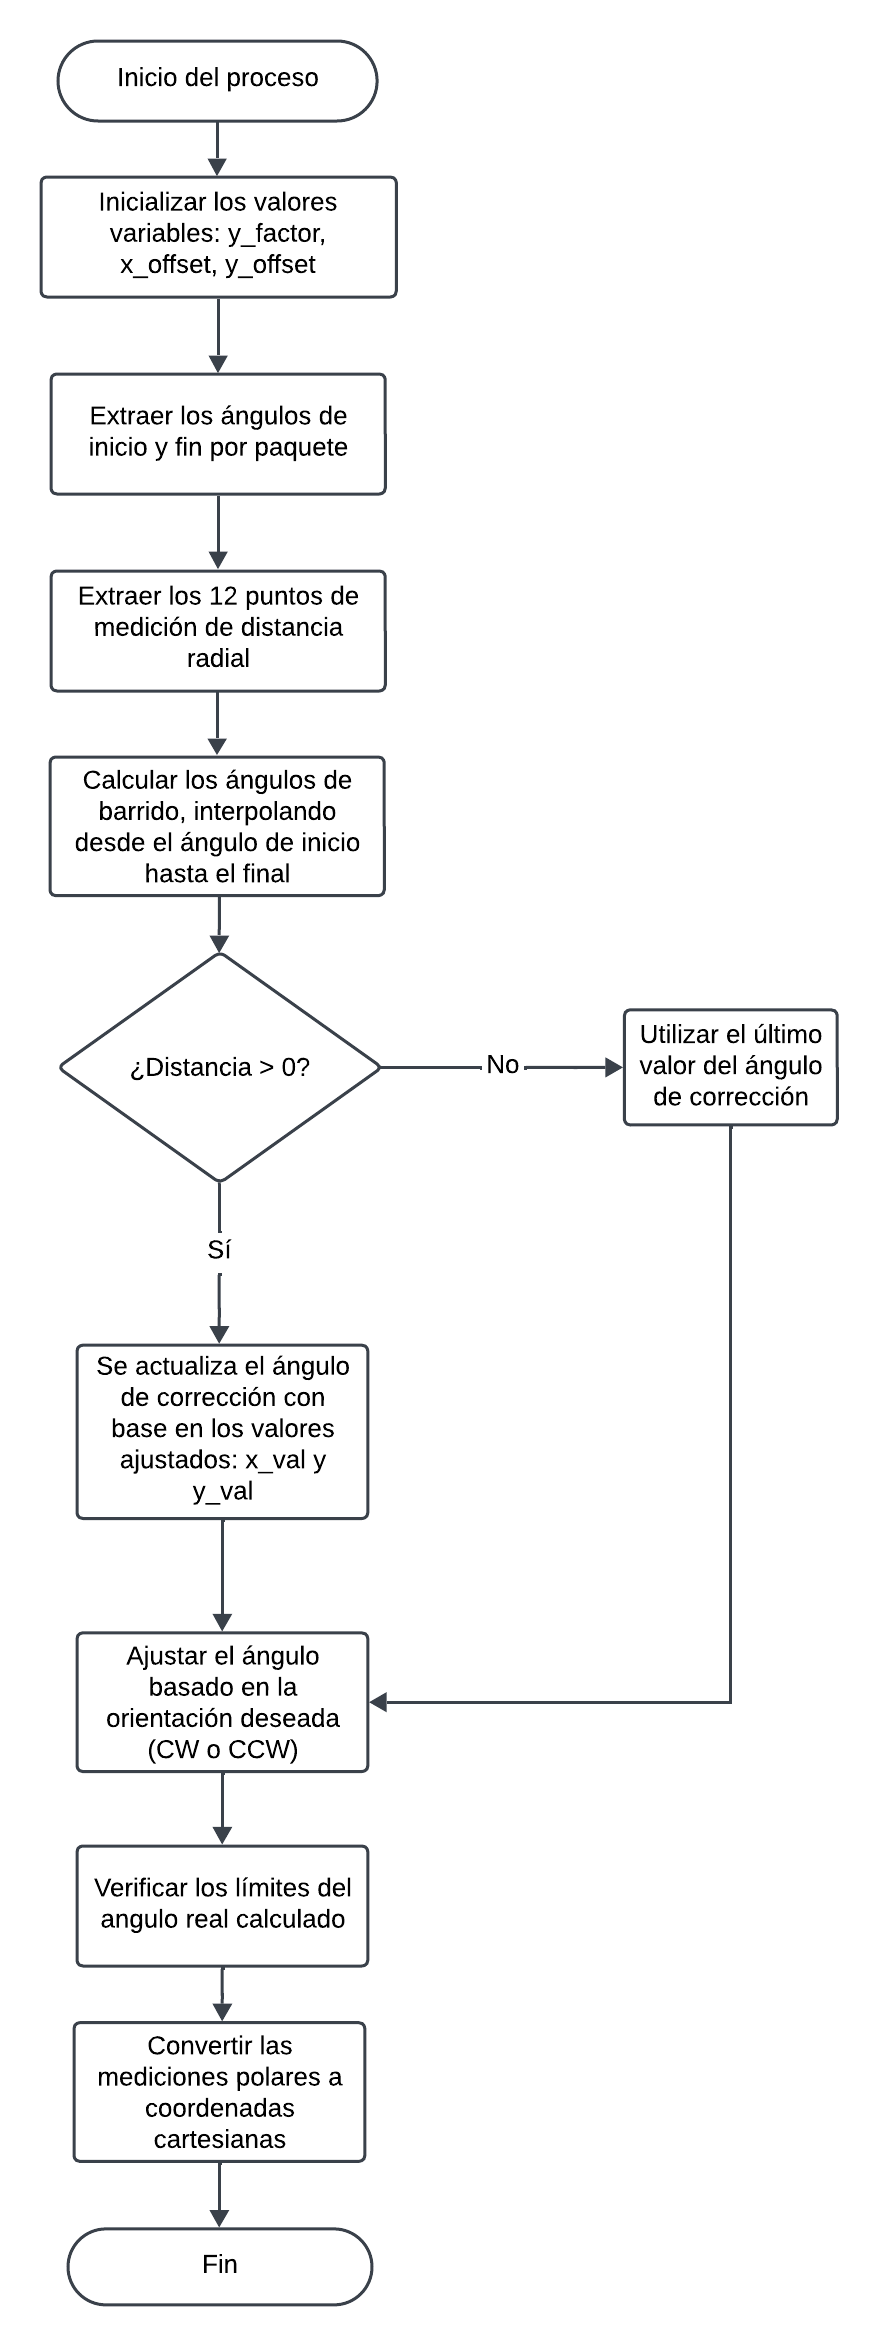
\includegraphics[width=0.4\textwidth]{diagrama_procesamiento_dec.png}
	\caption{Diagrama de flujo general para procesamiento de datos en formato decimal.}
	\label{fig:diagrama_procesamiento_dec}
\end{figure}

En caso de que la distancia medida sea igual a cero, no se recalculan los valores de ajuste, ya que la medición carece de información para ese punto. En su lugar, se reutiliza el último ángulo de corrección calculado, para ajustar el ángulo real de esa medición nula. Este procedimiento garantiza que incluso estas mediciones mantengan una continuidad angular coherente respecto a las anteriores, evitando distorsiones en la reconstrucción del entorno. Sin embargo, incluir estas mediciones nulas en los gráficos de coordenadas polares y cartesianas resulta innecesario, ya que, físicamente, el sensor no es capaz de registrar mediciones justo en su eje de rotación. 

Estos puntos añaden cierta confusión visual al interpretar el entorno capturado. Por esta razón, se optó por filtrar las mediciones cuya distancia radial fuese cero. Al eliminar estos puntos en la generación de los gráficos, se preservan solo las distancias que aportan información relevante sobre el entorno. Este filtrado mejora la claridad y precisión de la representación de los objetos detectados, lo cual mejora la interpretación de los datos capturados. En la Figura \ref{fig: comparación_con_sin_filt} se muestra la comparación antes y después de depurar las mediciones nulas capturadas.

\begin{figure}[H]
	\centering
	\begin{subfigure}{0.6\textwidth}
		\centering
		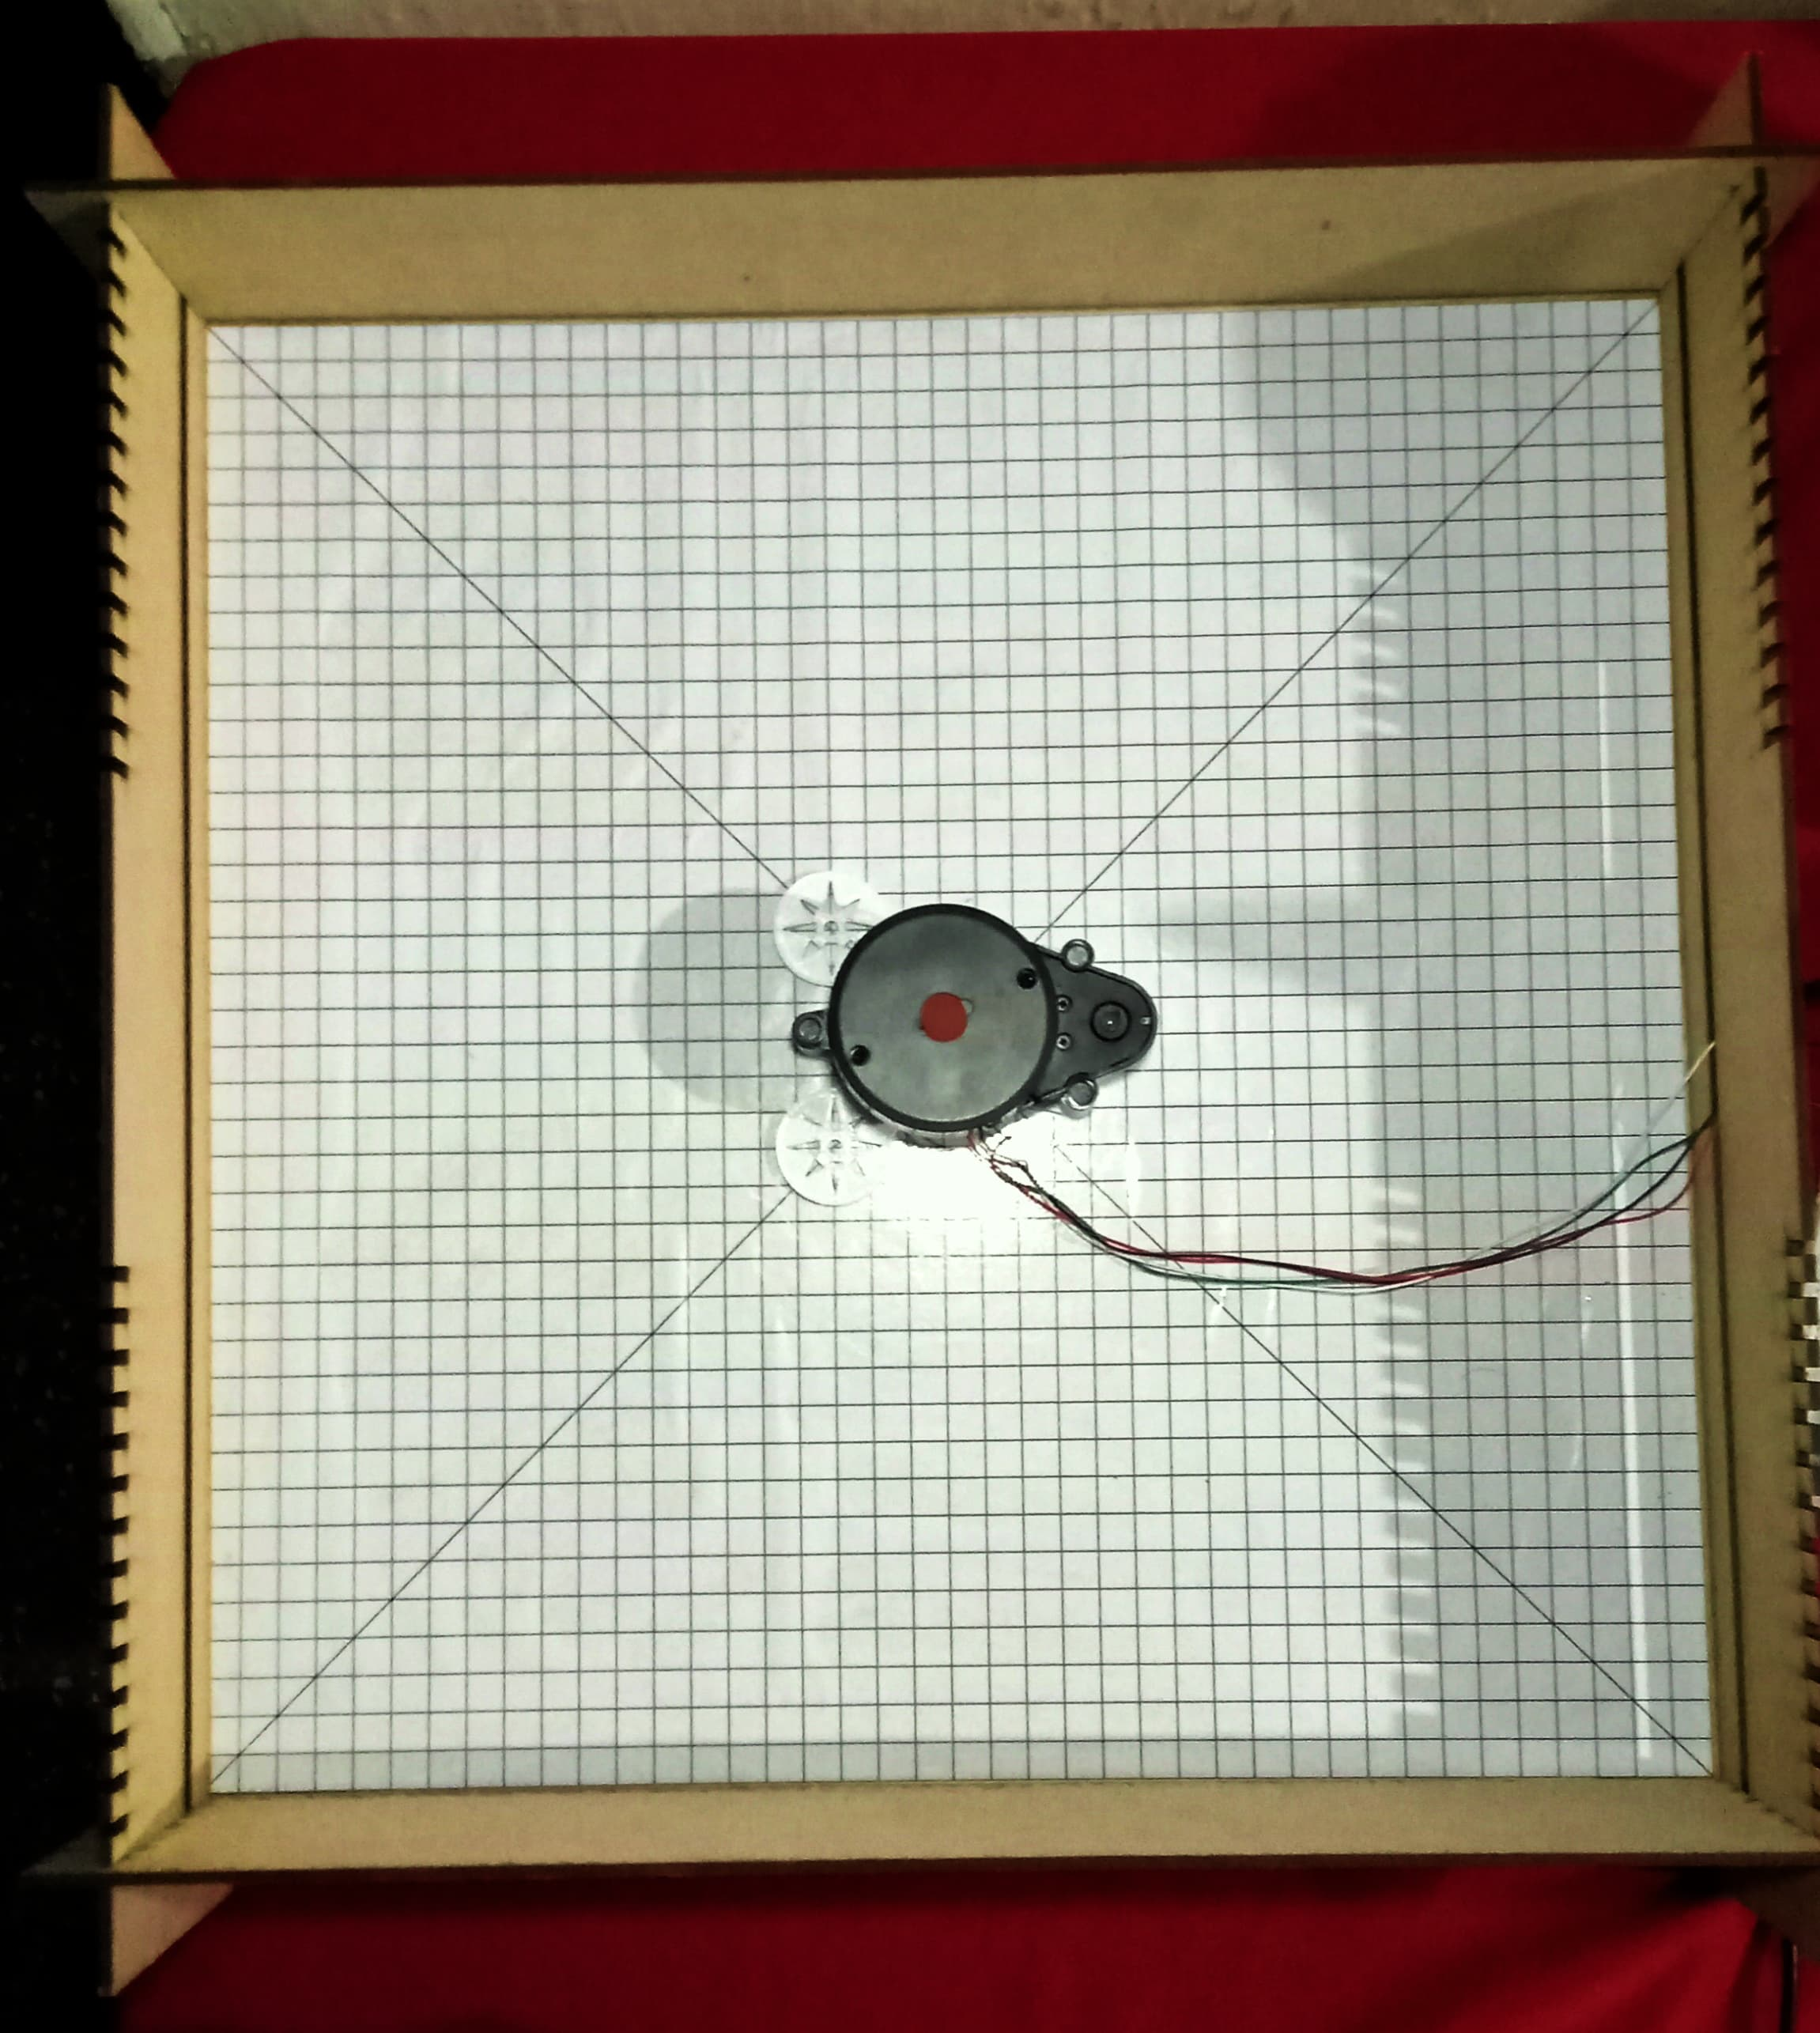
\includegraphics[width=0.7\linewidth]{disposicion_lidar3.jpeg}
		\caption{Disposición del sensor FHL-LD20 dentro de la caja.}
		\label{disposicion_lidar3}
		\vspace{1em}
	\end{subfigure}
	\begin{subfigure}{0.45\textwidth}
		\centering
		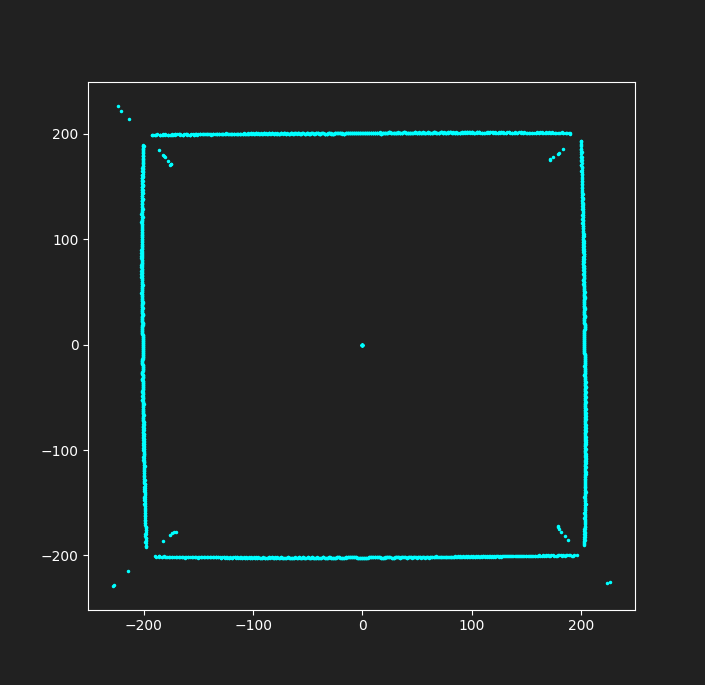
\includegraphics[width=0.9\linewidth]{lectura_sin_filt.png}
		\caption{Reconstrucción de tres revoluciones completas capturadas sin filtro de mediciones nulas.}
		\label{lectura_sin_filt}
	\end{subfigure}
	\hspace{1em}
	\begin{subfigure}{0.45\textwidth}
		\centering
		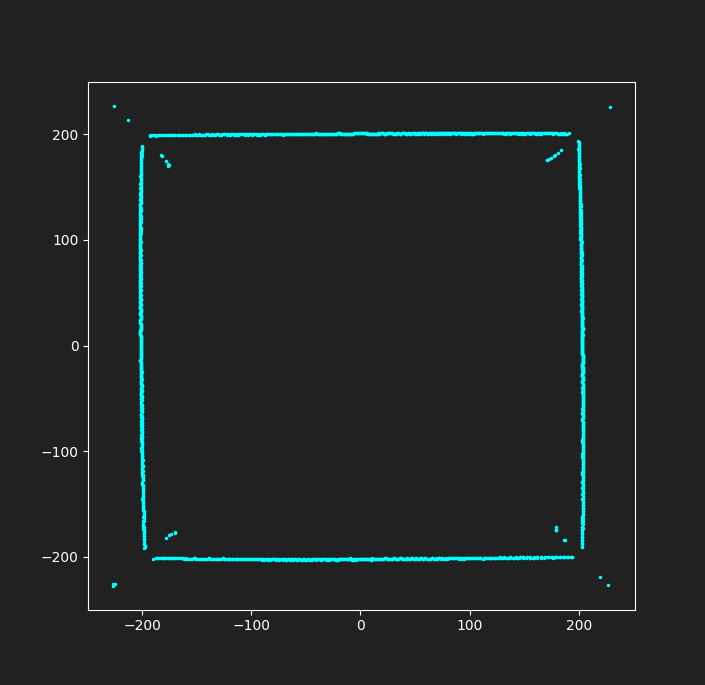
\includegraphics[width=0.9\linewidth]{lectura_con_filt.png}
		\caption{Reconstrucción de tres revoluciones completas capturadas con filtro de mediciones nulas.}
		\label{lectura_con_filt}
	\end{subfigure}
	\caption{Comparación de la reconstrucción con y sin filtro de mediciones nulas: tres revoluciones completas capturadas.}
	\label{fig: comparación_con_sin_filt}
\end{figure}

\section{Rango de medición efectivo del LiDAR FHL-LD20}
Determinar el rango de medición efectivo implica evaluar las distancias mínima y máxima a las que el sensor puede operar con precisión y confiabilidad. El rango mínimo de medición es fundamental para identificar las limitaciones del sensor en rangos cercanos, mientras que el rango máximo define l alcance que el sensor puede cubrir. Conocer estos rangos permite ajustar la caracterización del sensor para satisfacer las necesidades específicas de la aplicación en la que se utilizará.

\subsection{Rango mínimo de medición}
Para evaluar la distancia mínima que el sensor es capaz de medir, se diseñaron entornos circulares con diámetros cercanos a la distancia mínima especificada por el fabricante. Se imprimieron en 3D círculos de 6, 7, 8, 9, 10 y 11 cm de radio con el fin de identificar el rango mínimo que permitiera un funcionamiento adecuado del sensor. Optar por un contorno circular en lugar de uno cuadrado resultó ventajoso, ya que la naturaleza del sensor favorece una cobertura uniforme en todas las direcciones.

En la Figura \ref{fig: reconstrucciones_vacías_6} se muestra la primera prueba, realizada con un contorno circular de 6 cm de radio. Como se aprecia en las Figuras \ref{try_6cm_r} y \ref{try_6cm_r_car}, el contorno no pudo ser reconstruido, y las gráficas resultaron vacías. Al analizar los datos sin procesar de este experimento, se descubrió que el sensor no era capaz de registrar distancias válidas, por lo que se registraban como cero (ver Figura \ref{fig:data_null}). Y, debido a que las mediciones se filtraban para eliminar las distancias nulas, la reconstrucción de los datos resultó vacía. 

Es importante señalar que, a pesar de la ausencia de mediciones de distancia válidas, el sensor aún capturaba los ángulos de inicio y final, como se muestra en la Figura \ref{fig:data_null}. Esto sugiere que la cobertura del campo de visión del sensor es independiente de su capacidad para registrar distancias radiales válidas.
\begin{figure}[H]
	\centering
	
\includegraphics[width=0.8\textwidth]{lecturas_nula.jpg}
	\caption{Ejemplificación de las lecturas nulas durante la reconstrucción de mediciones: entorno circular de 6 cm de radio.}
	\label{fig:data_null}
\end{figure}

\begin{figure}[H]
	\centering
	\begin{subfigure}{0.6\textwidth}
		\centering
		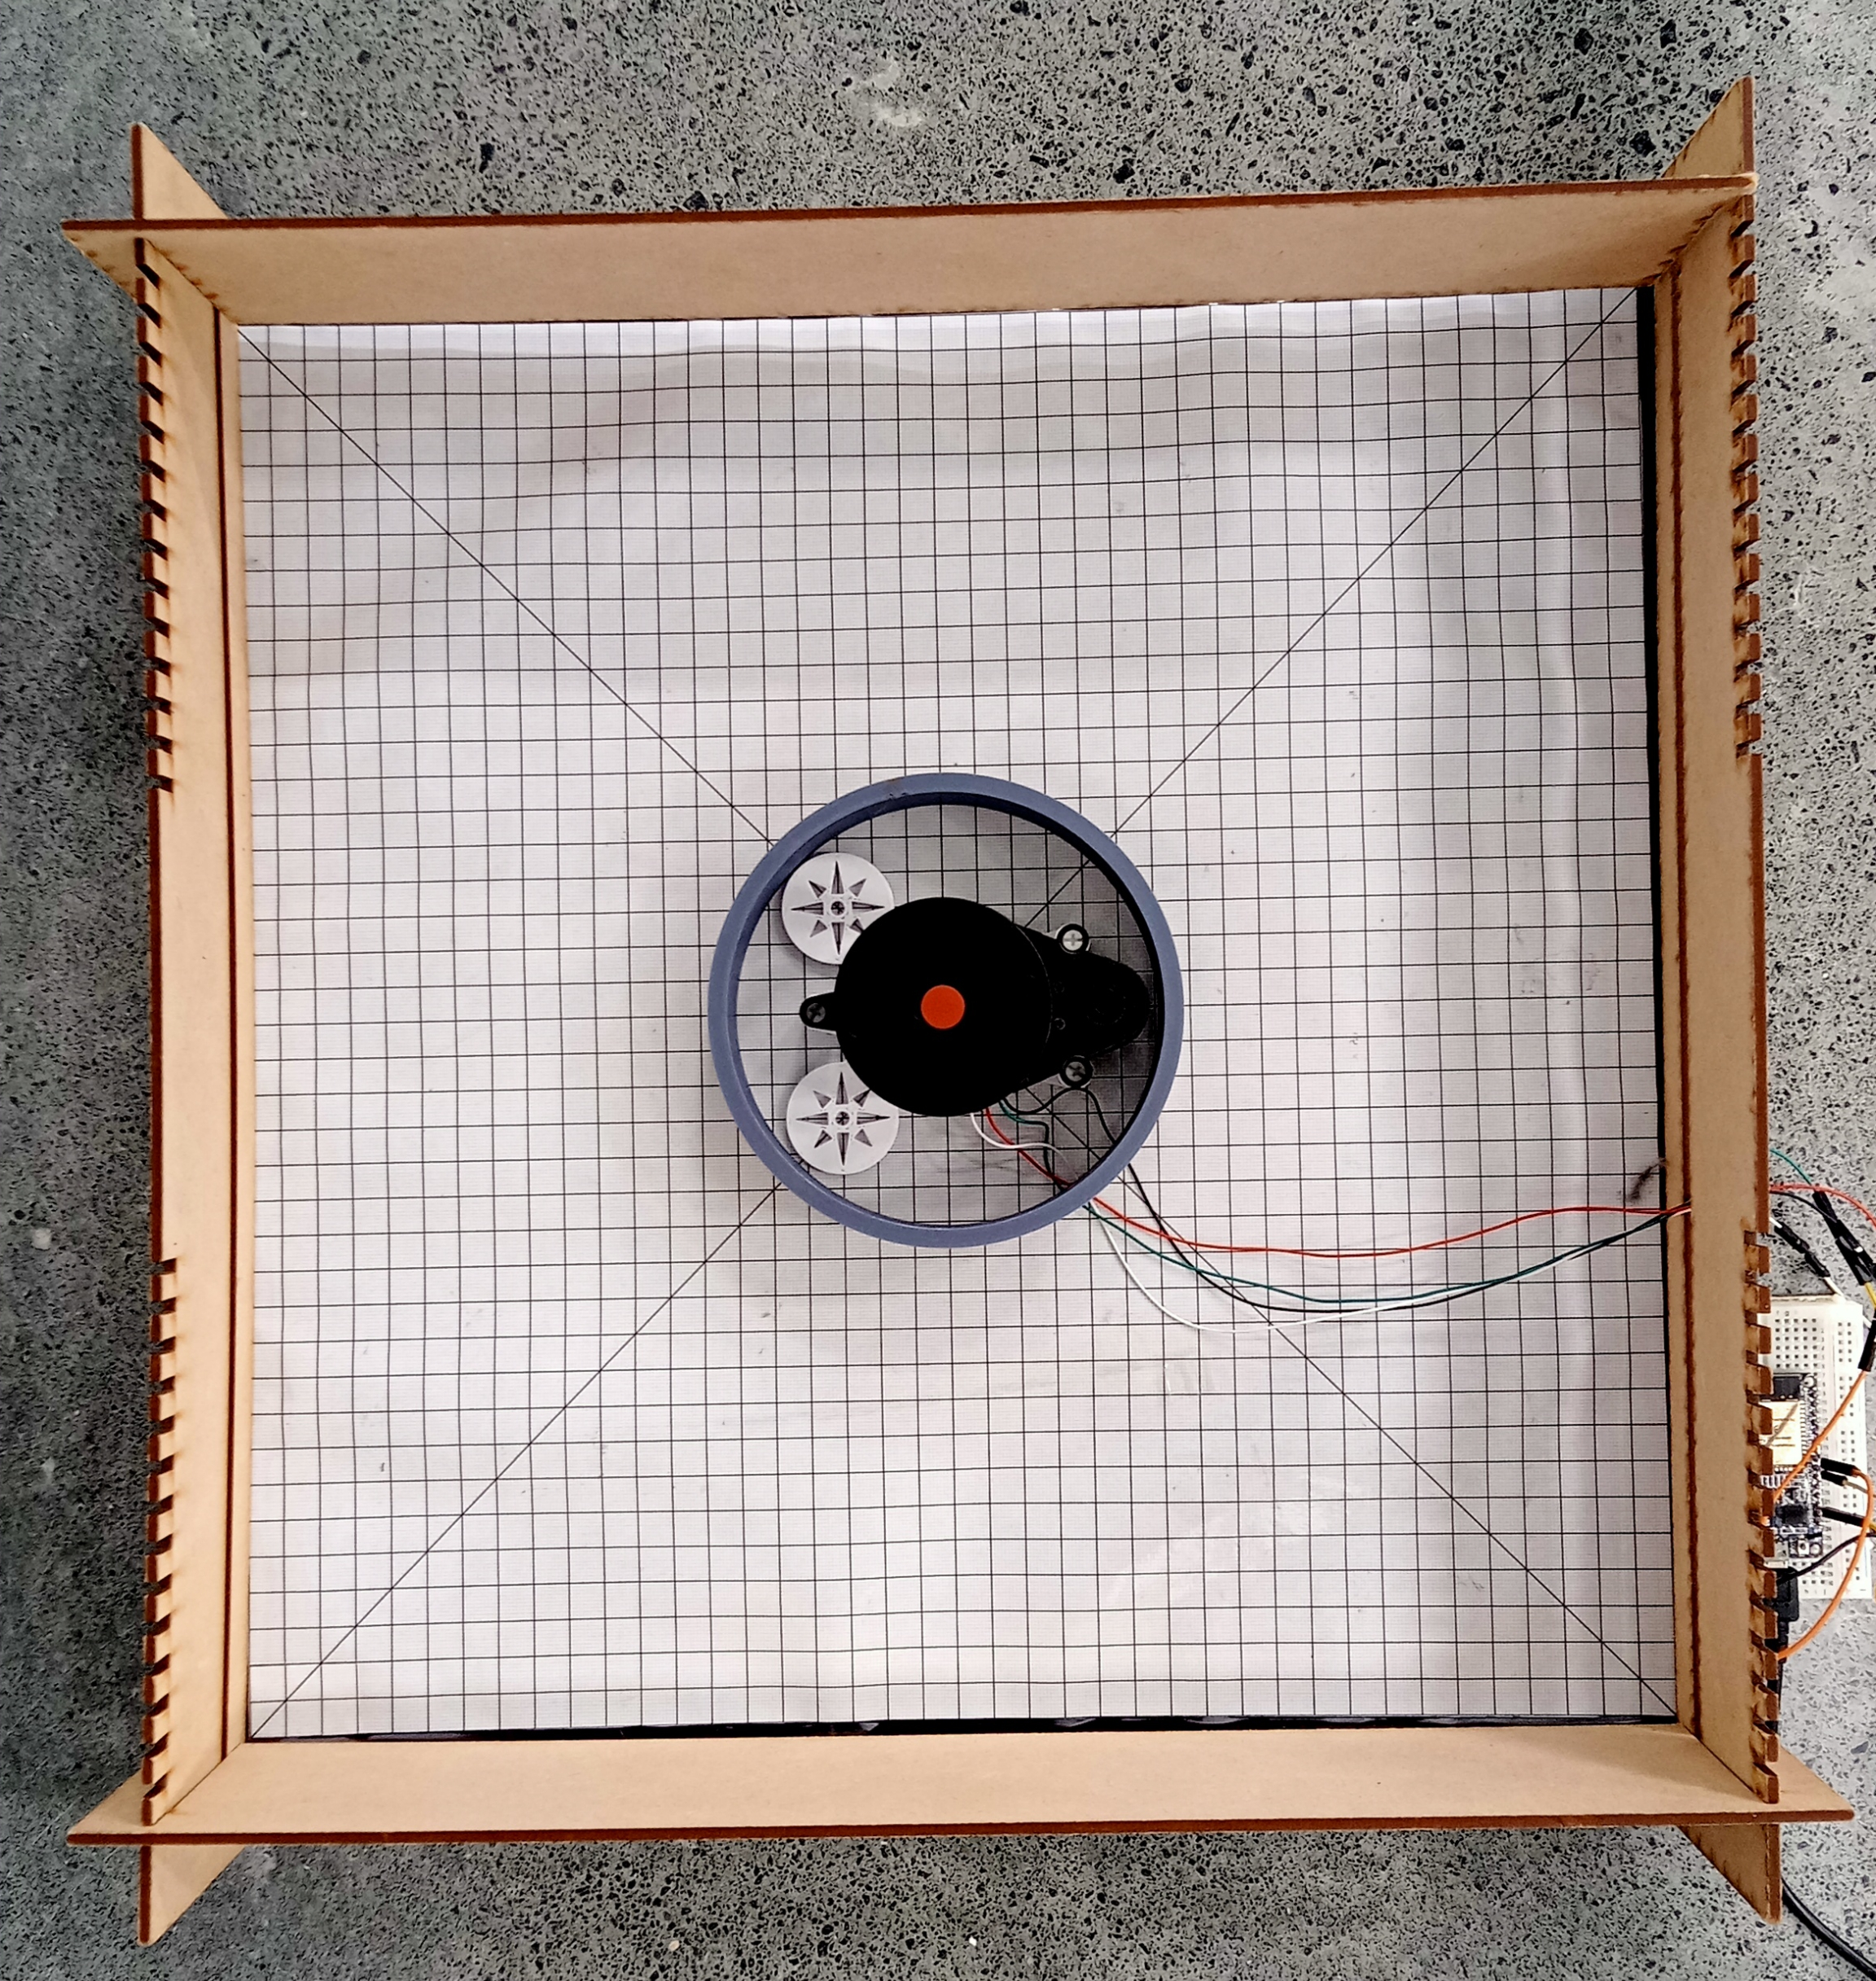
\includegraphics[width=0.65\linewidth]{disposicion_lidar4.jpeg}
		\caption{Disposición del sensor FHL-LD20 dentro del entorno circular: 6 cm de radio}
		\label{disposicion_lidar4}
		\vspace{1em}
	\end{subfigure}
	\begin{subfigure}{0.45\textwidth}
		\centering
		\includegraphics[width=0.9\linewidth]{try_6cm_r.png}
		\caption{Reconstrucción en coordenadas polares de tres revoluciones completas capturadas en entorno circular: 6 cm de radio}
		\label{try_6cm_r}
	\end{subfigure}
	\hspace{1em}
	\begin{subfigure}{0.45\textwidth}
		\centering
		\includegraphics[width=0.9\linewidth]{try_6cm_r_car.png}
		\caption{Reconstrucción en coordenadas cartesianas de tres revoluciones completas capturadas en entorno circular: 6 cm de radio}
		\label{try_6cm_r_car}
	\end{subfigure}
	\caption{Reconstrucciones vacías de tres revoluciones completas capturadas en entorno circular: 6 cm de radio}
	\label{fig: reconstrucciones_vacías_6}
\end{figure}


Se llevaron a cabo pruebas adicionales utilizando los contornos circulares de 7, 8, 9 y 10 cm de radio (ver Anexos \ref{fig: reconstrucciones_vacías_7} y \ref{fig: reconstrucciones_vacías_8}). El entorno circular de 9 cm de radio fue el primero en mostrar indicios de distancias válidas en la reconstrucción. No obstante, la geometría obtenida no resultó completamente precisa. Aunque se logra visualizar una geometría circular, esta presenta irregularidades. Como se observa en la Figura TAL, existen variaciones en la distribución de los puntos. 

A diferencia del resultado anterior, la reconstrucción del entorno de 10 cm de radio muestra una geometría más continua, ajustándose mejor a la forma esperada (ver Figura \ref{fig: reconstrucciones_10}). Este comportamiento era de esperarse, pues las especificaciones del fabricante indican un rango mínimo de medición de 10 cm. El entorno circular de 9 cm de radio, al estar por debajo del umbral mínimo de medición, refleja una mayor inexactitud, pues el sensor no se encuentra optimizado para capturar con precisión distancias tan cortas. 

\begin{figure}[H]
	\centering
	\begin{subfigure}{0.6\textwidth}
		\centering
		\includegraphics[width=0.65\linewidth]{disposicion_lidar8.jpeg}
		\caption{Disposición del sensor FHL-LD20 dentro del entorno circular: 10 cm de radio}
		\label{disposicion_lidar8}
		\vspace{1em}
	\end{subfigure}
	\begin{subfigure}{0.45\textwidth}
		\centering
		\includegraphics[width=0.9\linewidth]{try_10cm_r.png}
		\caption{Reconstrucción en coordenadas polares de tres revoluciones completas capturadas en entorno circular: 10 cm de radio}
		\label{try_10cm_r}
	\end{subfigure}
	\hspace{1em}
	\begin{subfigure}{0.45\textwidth}
		\centering
		\includegraphics[width=0.9\linewidth]{try_10cm_r_car.png}
		\caption{Reconstrucción en coordenadas cartesianas de tres revoluciones completas capturadas en entorno circular: 10 cm de radio}
		\label{try_10cm_r_car}
	\end{subfigure}
	\caption{Reconstrucciones vacías de tres revoluciones completas capturadas en entorno circular: 10 cm de radio}
	\label{fig: reconstrucciones_10}
\end{figure}

Para garantizar una detección eficiente y reducir el ruido causado por los componentes estructurales de los agentes robóticos donde se integrará el sensor, como es el caso del Pololu 3pi+, se ha establecido un rango mínimo de medición de 15 cm. A distancias inferiores a  esta, el sensor podría captar partes del propio robot, lo que afectaría negativamente la precisión de las mediciones. Además, dado que la probabilidad de encontrar obstáculos relevantes a menos de 10 cm en el entorno de operación es baja, establecer este límite permite enfocarse en la detección de obstáculos que realmente impacten en la navegación del agente robótico.

\subsection{Rango máximo de medición}
FALTAN HACER PRUEBAS EN UNA HABITACIÓN.

\section{Estimación de las varianzas del sensor }
\label{sec:estimacion}
En aplicaciones de mapeo de entornos con agentes robóticos móviles, la localización del robot depende de mediciones de distancia y ángulo hacia puntos de referencia fijos (\textit{landmarks}). Describir cómo un sensor de distancia, como un LIDAR, mide su posición relativa con respecto a estos puntos resulta esencial para construir un mapa coherente y actualizar la posición del robot en función de sus observaciones. Este enfoque permite corregir errores acumulados de odometría y reducir la incertidumbre en la estimación de posición, lo que posibilita que los agentes robóticos se localicen y mapeen su entorno de manera precisa y confiable \cite{corke_robotics_2017}. Para modelar matemáticamente las observaciones de un sensor de distancia equipado en un agente robótico, se emplea la Ecuación \eqref{eq:robot_landmark}.

\begin{equation}
	\label{eq:robot_landmark}
	z = h(x,p_i) 
\end{equation}

donde $x = (x_v, y_v, \theta_v)^T$ representa el estado del agente robótico, con $x_v$ y $y_v$ como sus coordenadas en el sistema global y $\theta_v$ como su orientación. Mientras que $p_i = (x_i, y_i)^T$ denota la posición conocida del i-ésimo punto de referencia en el entorno. Para modelar la incertidumbre en las mediciones de distancia y ángulo, la Ecuación \eqref{eq:robot_landmark2} extiende el modelo de observación, añadiendo un vector de ruido que refleja los errores en estas mediciones.

\begin{equation}
	\label{eq:robot_landmark2}
	z = h(x, p_i) =
	\begin{pmatrix}
		\sqrt{(y_i - y_v)^2 + (x_i - x_v)^2} \\
		\tan^{-1}\left(\frac{y_i - y_v}{x_i - x_v}\right) - \theta_v
	\end{pmatrix}
	+
	\begin{pmatrix}
		w_r \\
		w_\beta
	\end{pmatrix}
\end{equation}

\begin{equation}
	\label{eq:matriz_covarianza}
	\begin{pmatrix}
		w_r \\
		w_\beta
	\end{pmatrix}
	\sim
	N(0,W),	W =
	\begin{pmatrix}
		\sigma_r^2 & 0 \\
		0 & \sigma_\beta^2
	\end{pmatrix}
\end{equation}

Esta ecuación describe cómo el sensor mide la distancia $r$ y el ángulo $\beta$ al punto de referencia $p_i$, incorporando un vector de ruido en las mediciones. Este modelo asume que los errores $w_r$ y $w_\beta$ siguen  una distribución Gaussiana con media cero y varianza conocida en las mediciones de distancia y ángulo, respectivamente. En la Ecuación \ref{eq:matriz_covarianza} se especifica la matriz de covarianza $W$, en la cual $\sigma_r^2$ representa la varianza del error en la distancia y $\sigma_\beta^2$ la varianza del error en el ángulo. Esta matriz de covarianza refleja que las observaciones del sensor están sujetas a una incertidumbre inherente.

Para estimar las varianzas $\sigma_r^2$ y $\sigma_\beta^2$ se llevaron a cabo dos experimentos con el sensor LIDAR FHL-LD20.  El primero se centró en evaluar la varianza asociada a las mediciones de distancia, mientras que el segundo se enfocó en analizar las mediciones angulares. Ambos experimentos fueron diseñados para proporcionar una comprensión más profunda del rendimiento del sensor y su precisión en condiciones de operación.

\subsection{Estimación de la varianza asociada a las mediciones de distancia del sensor}
Para el primer experimento, se diseñaron ocho círculos concéntricos con radios de 150, 200, 250, 300, 350, 400, 450 y 500 mm, todos con una altura de 70 mm. Estos círculos fueron fabricados en MDF y recubiertos con una capa uniforme de cartón de 1 mm de grosor. Además, se imprimió una cuadrícula de 1.2$\times$1.2 metros, dividida en intervalos de un centímetro. Esta cuadrícula incluía una serie de círculos concéntricos con los radios mencionados y líneas diagonales que cruzaban su centro, creando un sistema de referencia radial. En conjunto, este diseño ofreció un entorno ideal para analizar las mediciones en coordenadas polares y cartesianas.

\begin{figure}[H]
	\centering
	\begin{subfigure}{\textwidth}
		\centering
		\makebox[\textwidth]{\includegraphics[width=0.6\linewidth]{disposicion_lidar_var_dist1.jpg}}
		\caption{Disposición del sensor FHL-LD20 dentro del entorno circular: 149 mm de radio}
		\label{fig:disposicion_lidar_var1}
		\vspace{1em}
	\end{subfigure}
	\begin{subfigure}{0.45\textwidth}
		\centering
		\includegraphics[width=0.8\linewidth]{0.149m_radius.png}
		\caption{Reconstrucción en coordenadas polares de entorno circular: 149 mm de radio}
		\label{fig:149m_radius_xy}
	\end{subfigure}
	\hspace{1em}
	\begin{subfigure}{0.45\textwidth}
		\centering
		\includegraphics[width=0.83\linewidth]{0.149m_radius_XY.png}
		\caption{Reconstrucción en coordenadas cartesianas de entorno circular: 149 mm de radio}
		\label{fig:149m_radius}
	\end{subfigure}
	\caption{Reconstrucción con 180 revoluciones completas capturadas del entorno circular: 149 mm de radio.}
	\label{fig:disposicion_lidar_var_dist1}
\end{figure}

\begin{figure}[H]
	\centering
	\begin{subfigure}{\textwidth}
		\centering
		\makebox[\textwidth]{\includegraphics[width=0.6\linewidth]{disposicion_lidar_var_dist8.jpg}}
		\caption{Disposición del sensor FHL-LD20 dentro del entorno circular: 499 mm de radio}
		\label{fig:disposicion_lidar_var8}
		\vspace{1em}
	\end{subfigure}
	\begin{subfigure}{0.45\textwidth}
		\centering
		\includegraphics[width=0.8\linewidth]{0.499m_radius.png}
		\caption{Reconstrucción en coordenadas polares de entorno circular: 499 mm de radio}
		\label{fig:449m_radius_xy}
	\end{subfigure}
	\hspace{1em}
	\begin{subfigure}{0.45\textwidth}
		\centering
		\includegraphics[width=0.83\linewidth]{0.499m_radius_XY.png}
		\caption{Reconstrucción en coordenadas cartesianas de entorno circular: 499 mm de radio}
		\label{fig:449m_radius}
	\end{subfigure}
	\caption{Reconstrucción del entorno circular de 499 mm de radio con 180 revoluciones completas capturadas.}
	\label{fig:disposicion_lidar_var_dist8}
\end{figure}

Como se muestra en las Figuras \ref{fig:disposicion_lidar_var_dist1} y \ref{fig:disposicion_lidar_var_dist8}, el sensor se posicionó en el centro de la cuadrícula y se alineó concéntricamente uno de los círculos fabricados, utilizando las líneas radiales como guía. Con esta disposición se esperaba que el sensor registrara mediciones uniformes a lo largo de todo el perímetro del círculo. Después de capturar un total de 180 revoluciones, equivalente a 129,600 puntos de medición, y repetir diez veces las mediciones, fue posible establecer el promedio, varianza muestral y sesgo asociados con las distancias medidas por el sensor para cada círculo. El análisis de los datos obtenidos con los ocho círculos permitió evaluar la la precisión del sensor a distintas distancias, proporcionando una base sólida para caracterizar la variabilidad en las mediciones y determinar la varianza asociada en cada caso.

Los resultados del experimento se presentan en el Cuadro \ref{cuadro:stats}, donde se muestran las varianzas calculadas para cada uno de los ocho radios evaluados. En todos los casos, se verificó que las mediciones se ajustaran a una distribución gaussiana normal (ver Anexos), lo que respalda la validez del modelo de ruido asumido para las observaciones del sensor (Sección \ref{sec:estimacion}). Además, se observó que, a medida que aumentaba la distancia de los radios, también se incrementaba la varianza en las mediciones, indicando una disminución gradual en la exactitud del sensor. Para caracterizar esta relación, se realizó un ajuste lineal de los datos, como se muestra en la Figura \ref{fig:varianza_tendencia}, lo que permitió describir la variación de la varianza en función de la distancia. Es importante señalar que el valor esperado para cada medición resultó ser 1 mm menor que el radio del círculo evaluado debido al grosor del recubrimiento de cartón. 

\begin{table}[H]
	\centering
	\resizebox{\textwidth}{!}{\begin{tabular}{|c|c|c|c|}
		\hline
		\textbf{Radio real ($mm$)} & \textbf{\makecell{Promedio de mediciones \\capturadas ($mm$)}} & \textbf{Bias ($mm$)} & \textbf{\makecell{Varianza \\muestral ($mm^2$)}} \\ \hline
		\textbf{499} & 499.2150 & -0.7850 & 2.4503 \\ \hline
		\textbf{449} & 448.5695 & -0.4306 & 1.4682 \\ \hline
		\textbf{399} & 398.3953 & -0.6047 & 1.3529 \\ \hline
		\textbf{349} & 348.0344 & -0.9656 & 1.0317 \\ \hline
		\textbf{299} & 298.0343 & -0.9657 & 0.5360 \\ \hline
		\textbf{249} & 249.1742 & 0.1742 & 0.5493 \\ \hline
		\textbf{199} & 199.9887 & 0.9895 & 0.4950 \\ \hline
		\textbf{149} & 148.9746 & -0.0254 & 0.0970 \\ \hline
	\end{tabular}}
	\caption{Estadísticas de precisión: valores promedio de distancia, sesgo y varianza muestral obtenidos para cada radio tras las diez corridas realizadas.} 
	\label{cuadro:stats}
\end{table}

\begin{figure}[H]
	\centering
	\includegraphics[width=0.8\textwidth]{varianza_tendencia.png}
	\caption{Ajuste lineal para la variación de la varianza en función de la distancia.}
	\label{fig:varianza_tendencia}
\end{figure}

En la Figura \ref{fig:lecturas1}, se aprecia que para el primer círculo, con un radio real de 149 mm, la variabilidad de los puntos medidos fue relativamente baja, con una notable concentración de mediciones cercanas al valor esperado (149 mm). Sin embargo, al aumentar el radio medido, la dispersión de los puntos incrementó, reflejando una mayor variabilidad en las mediciones (ver Figura \ref{fig:lecturas2}). En cuanto al sesgo o \textit{bias}, la Figura \ref{fig:bias_tendencia} demuestra que no se identificó una tendencia clara, ya que este oscilaba entre aproximadamente -0.9657 mm y 0.9895 mm. Es importante destacar que la varianza muestral, promedio y sesgo reportados en el Cuadro \ref{cuadro:stats} representan los promedios obtenidos en las diez corridas realizadas, proporcionando así una estimación robusta de las mediciones en cada radio. Para una comprensión más detallada de los resultados, en los Anexos TALES se encuentran las estadísticas completas de cada corrida realizada.


\begin{figure}[H]
	\centering
	\makebox[\textwidth]{\includegraphics[width=1.25\linewidth]{0.149m_radius_stats_P6.png}}
	\caption{Variabilidad de las mediciones capturadas para un radio real de 149 mm.}
	\label{fig:lecturas1}
\end{figure}

\begin{figure}[H]
	\centering
	\makebox[\textwidth]{\includegraphics[width=1.25\linewidth]{0.499m_radius_stats_P1.png}}
	\caption{Variabilidad de las mediciones capturadas para un radio real de 499 mm.}
	\label{fig:lecturas2}
\end{figure}

\begin{figure}[H]
	\centering
	\includegraphics[width=0.8\textwidth]{bias_tendencia.png}
	\caption{Variación del sesgo en función de la distancia.}
	\label{fig:bias_tendencia}
\end{figure}

\subsection{Estimación de la varianza asociada a las mediciones de ángulos del sensor}
En el segundo experimento, se utilizó el mismo conjunto de círculos fabricados para el primer experimento, añadiendo un noveno círculo de 70 mm de radio, diseñado para obstruir la visión del sensor en ciertas direcciones. Como se muestra en las Figuras TAL y TAL, el sensor se mantuvo estático en el centro de la cuadrícula, mientras se colocaban dos círculos: uno externo, correspondiente a los fabricados previamente, y el círculo de obstrucción visual, que incluía ligera abertura de 30°. Adicionalmente, se colocó un arco circular con un radio 20 mm menor que el del círculo externo, cubriendo un rango angular de 42° a 47°. Esta disposición permitió evaluar si el LiDAR era capaz de medir adecuadamente los ángulos según el arco establecido. 

Para cada círculo externo, se realizaron diez corridas del experimento, generando un conjunto de datos para evaluar la precisión angular del sensor. Como se detalla en el Cuadro TAL, se observa cierta variabilidad respecto a los valores reales de inicio y final del arco (42° y 47°, respectivamente), lo que indica una variación sistemática en las mediciones angulares del sensor. Al analizar la distribución de las mediciones angulares, se determinó que los datos seguían una distribución normal (ver Anexos), lo cual hace inapropiado el uso de la varianza tradicional para representar la dispersión. En su lugar, en el Cuadro TAL se deja indicado la diferencia respecto a los valores teóricos.

\section{Precisión del LiDAR FHL-LD20}
Para evaluar la precisión del sensor en las mediciones de distancias y ángulos, se llevó a cabo un análisis basado en la reconstrucción de cajas de diferentes dimensiones. Este proceso incluyó la determinación de regresiones lineales para las aristas detectadas y el cálculo de diversas métricas que permiten evaluar la fidelidad de las mediciones del sensor. A continuación se detalla el proceso para evaluar la precisión del sensor para una caja de 400 $\times$ 400 mm.

En primer lugar, se aplicó un filtro para seleccionar los puntos más cercanos a las aristas esperadas, utilizando un intervalo de tolerancia de $\pm$ 5 mm. Se excluyó una franja cercana a los bordes de la caja para evitar distorsiones derivadas al efecto de las esquinas, que suelen generar mediciones menos precisas debido a la complejidad de la geometría de estas áreas. Posteriormente, se realizó un ajuste de regresión lineal para cada conjunto de puntos que conformaba una arista de la caja reconstruida. En el caso de las aristas horizontales, el valor de los valores en el eje Y se ajustó en función de los valores del eje X. Mientras que, para las aristas verticales, se ajustaron los valores del eje X en función de los valores del eje Y. 

A partir de los puntos filtrados y las regresiones obtenidas, se calcularon las siguientes métricas para cada arista:
\begin{itemize}
	\item Ecuación de la recta: Pendiente e intercepto obtenidos a partir del ajuste lineal.
	\item Error cuadrático medio entre los puntos reales y la línea ajustada.
	\item Intervalos de confianza (IC): Para la pendiente e intercepto, se calcularon intervalos de confianza del 95\%, proporcionando una medida de la incertidumbre en la estimación de los parámetros de la recta.
	\item Diferencia promedio. Media de las diferencias entre los puntos detectados y el valor real esperado, proporcionando una medida del error sistemático del sensor.
	\item Puntos máximo y mínimo: Los valores extremos detectados en cada conjunto de puntos que indican la variabilidad en las mediciones.
	\item Rango: Diferencia entre el valor máximo y mínimo., lo que refleja la dispersión de las mediciones.
\end{itemize}

Para evaluar la rectitud de las aristas, se analizaron las pendiente obtenidas a partir del ajuste lineal. Estas pendientes, muestran pequeñas desviaciones respecto a la horizontalidad o verticalidad ideal, lo que sugiere un ligero error sistemático en la orientación del sensor. Los intervalos de confianza calculados para estas presentan un rango estrecho, lo que indica una alta consistencia en las mediciones y un bajo nivel de variabilidad entre los diferente puntos medidos. Adicionalmente, las magnitudes de las pendientes están cercanas a cero, lo que sugiere que las aristas reconstruidas se aproximan de manera precisa a la geometría esperada (lineas rectas definidas). 

El intercepto calculado resulta útil para evaluar el alineamiento general del sensor con respecto a las posiciones esperadas. En todos los casos, se observan ligeras desviaciones en el intercepto que oscilan entre 0.3959 mm y 2.4565 mm con respecto a las dimensiones esperadas de  $\pm$ 200 mm, lo cual es relativamente bajo. Sin embargo, estas pequeñas variaciones evidencia la presencia de imprecisiones en las mediciones del sensor.

El análisis de los intervalos de confianza de la pendiente y eñ intercepto proporciona una medida de la fiabilidad de estos parámetros. Al mostrar rangos estrechos, se sugiera una fuerte consistencia en las mediciones, lo cual refuerza la confiabilidad de las regresiones lineales obtenidas. Junto a esto, el rango de las mediciones, que varía entre 3.8049 mm y 4.4322 mm para las diferentes aristas, refleja una dispersión controlada. La diferencia promedio entre los puntos detectados y el valor real esperado, inferior a 3 mm, confirma que la dispersión de las mediciones se encuentra dentro de los límites de precisión indicados por el fabricante. 

En resumen, las métricas analizadas muestran que el sensor presenta una buena precisión general. A pesar que se observen pequeñas desviaciones, los errores están por debajo de los 5 mm, lo cual es aceptable para la mayoría de las aplicaciones, en especial para navegación autónoma.

\begin{figure}[H]
	\centering
	\begin{subfigure}{0.8\textwidth}
		\centering
		\includegraphics[width=0.9\linewidth]{analisis_precision_1_1.png}
		\caption{Análisis de arista horizontal superior}
		\label{analisis_precision_1_1}
	\end{subfigure}
	\hspace{1em}
	\begin{subfigure}{0.8\textwidth}
		\centering
		\includegraphics[width=0.9\linewidth]{analisis_precision_1_2.png}
		\caption{Análisis de arista horizontal inferior}
		\label{analisis_precision_1_2}
		\vspace{1em}
	\end{subfigure}
	\caption{Análisis de la reconstrucción realizada para las aristas horizontales de una caja de 400$\times$400 mm: tres revoluciones completas capturadas.}
	\label{fig: reconstruccion_analisis_horizontal_1}
\end{figure}
\begin{figure}[H]
	\centering
	\begin{subfigure}{0.45\textwidth}
		\centering
		\includegraphics[width=1\linewidth]{analisis_precision_1_3.png}
		\caption{Análisis de arista vertical derecha}
		\label{analisis_precision_1_3}
	\end{subfigure}
	\hspace{1em}
	\begin{subfigure}{0.45\textwidth}
		\centering
		\includegraphics[width=1\linewidth]{analisis_precision_1_4.png}
		\caption{Análisis de arista vertical izquierda}
		\label{analisis_precision_1_4}
	\end{subfigure}
	\caption{Análisis de la reconstrucción realizada para las aristas verticales de una caja de 400$\times$400 mm: tres revoluciones completas capturadas.}
	\label{fig: reconstruccion_analisis_vertical_1}
\end{figure}

\section{Detección de bordes y discontinuidades para el LiDAR FHL-LD20}
A lo largo de los experimentos realizados se observó que, al probar con entornos cuadriláteros, las esquinas tienden a perderse en las mediciones. Esto sugiere que el sensor podría enfrentar dificultades para detectar con precisión bordes y discontinuidades en estas áreas específicas. Esto se debe a que las esquinas suele generar geometrías complejas y abruptas, lo que genera retornos dispersos e inconsistentes al interactuar con el haz infrarrojo.

Con e fin de evaluar cómo afectan las esquinas la precisión en las mediciones de los bordes, se diseñaron codos con radios de 5, 10 y 15 mm (Figura \ref{fig: codos}). Estos codos permiten estudiar el comportamiento del sensor cuando frente a transiciones suaves entre superficies, simulando una curvatura en lugar de un ángulo agudo. Al utilizar codos en lugar de esquinas afiladas, es posible analizar si el sensor puede detectar transiciones graduales en los bordes con mayor precisión, lo que reduce las distorsiones capturadas. Además, los codos proporcionan un medio de comparación para evaluar el rendimiento del sensor al medir bordes con radios de curvatura específicos, lo que permite establecer un rango de tolerancia en el cual las mediciones del sensor sean confiables.

\begin{figure}[H]
	\centering
	\begin{subfigure}{0.45\textwidth}
		\centering
		\includegraphics[width=0.9\linewidth]{codo.png}
		\caption{Vista isométrica del diseño del codo para transiciones graduales.}
		\label{codo}
	\end{subfigure}
	\hspace{1em}
	\begin{subfigure}{0.45\textwidth}
		\centering
		\includegraphics[width=0.9\linewidth]{codo3.png}
		\caption{Vista superior del diseño del codo de 5 mm de radio.}
		\label{codo3}
		\vspace{1em}
	\end{subfigure}
	\begin{subfigure}{0.45\textwidth}
		\centering
		\includegraphics[width=0.9\linewidth]{codo1.png}
		\caption{Vista superior del diseño del codo de 10 mm de radio.}
		\label{codo1}
	\end{subfigure}
	\hspace{1em}
	\begin{subfigure}{0.45\textwidth}
		\centering
		\includegraphics[width=0.9\linewidth]{codo2.png}
		\caption{Vista superior del diseño del codo de 15 mm de radio.}
		\label{codo2}
	\end{subfigure}
	\caption{Diseño de los codos para transiciones graduales}
	\label{fig: codos}
\end{figure}

\chapter{Calibración del LiDAR FHL-LD20}

\section{Pruebas para calibrar el LiDAR FHL-LD20}
Para verificar la calibración del sensor, se colocó en el centro de la plataforma utilizando las brújulas incluidas en el soporte para asegurar su alineación. Una vez posicionado, se realizó una captura de tres revoluciones completas y se compararon los valores medidos de las aristas con los valores nominales esperados. Si los resultados obtenidos se encuentran dentro de una desviación igual o menor a la precisión especificada por el radio de medición, se considera que el sensor está calibrado. En este experimento, se obtuvieron los siguientes mediciones de las aristas: 201.28 mm para la arista horizontal superior, -201.38 mm para la inferior, 202.45 mm para la vertical derecha, y -200.39 mm para la izquierda. Estas desviaciones, aunque mínimas, se encuentran dentro del rango de precisión del sensor, lo que confirma que el dispositivo está correctamente calibrado. 

\begin{figure}[H]
	\centering
	\includegraphics[width=0.5\textwidth]{calibracion1.png}
	\caption{Reconstrucción realizada para verificar la calibración del sensor.}
	\label{fig:calibracion}
\end{figure}

\section{Compensación en las mediciones del LiDAR FHL-LD20}
\label{sec:calibracion}

En la primera reconstrucción realizada (Figura \ref{primera_corrida}), se observaron deformaciones en las aristas de la caja, que no coincidían con los bordes rectos de la caja física. Estas deformaciones fueron causadas por la falta de corrección angular debida al desplazamiento físico del emisor/receptor del láser dentro de la carcasa. Este desplazamiento implica que el punto exacto desde donde se emite el láser y donde el sensor recoge las reflexiones está ligeramente descentrado con respecto al eje de rotación del sensor.

Cuando el láser no se emite desde el centro del círculo ideal que describe el barrido del LiDAR, se produce un desfase que afecta la precisión angular. Sin embargo, este desplazamiento interno no afecta la distancia medida, ya que sigue siendo una medición directa entre el sensor y el objeto. La luz viaja y vuelve directamente, similar a cómo se usaría una regla para medir la distancia en línea recta. El problema radica en que, un desfase angular interno provoca que el punto aparezca en una ubicación incorrecta en el plano, es decir, más a la izquierda o derecha de su verdadera posición.

El hecho que el sensor gira sobre un eje para medir diferentes ángulos, si el sensor se encuentra desplazado de ese centro de rotación, los ángulo medidos no representarán correctamente la posición de los objetos en el entorno. Para corregir este error, en la documentación proporcionada por el fabricante, se sugería consultar el proceso de corrección realizado a partir del código fuente (FALTA REF). En este se utilizan dos valores ajustados: x\_val y y\_val, que incorporan los desplazamientos en los ejes X y Y. Estos valores no son las coordenadas cartesianas de cada punto evaluado, sino ajustes que ayudan a calcular el error angular causado por el desfase físico del sensor. 

\begin{equation}
	\label{eq:valor_ajustado_x}
	x\_val = distancia + x\_offset
\end{equation}
\begin{equation}
	\label{eq:valor_ajustado_y}
	y\_val = distancia\times y\_factor + y\_offset
\end{equation}

En la Ecuación \ref{eq:valor_ajustado_y}, el valor ajustado y\_val utiliza una constante  ``y\_factor'' de 0.11923. Aunque la documentación no especifica la razón exacta de este valor, se puede inferir que su propósito era corregir la proyección angular de las mediciones. Probablemente compensando una inclinación natural del sensor o representando un ajuste empírico destinado a mejorar la precisión de las mediciones. A partir de los valores ajustados, se calcula un ángulo de corrección usando la función arcotangente de la relación y\_val sobre x\_val. Este ángulo de corrección refleja cuánto debe sumarse o restarse al ángulo original para compensar el desplazamiento interno del sensor. 

Si el sistema utiliza coordenadas en sentido antihorario, el angulo se invierte (restándole 360 grados) y luego se suma el ángulo de corrección para obtener el valor final. En caso contrario, el ángulo de corrección se resta directamente del ángulo original. La Figura \ref{fig: comparación_con_sin_corre}, muestra la disposición del sensor dentro de la caja, junto con una comparación de la reconstrucción visual obtenida a partir de tres revoluciones completas capturadas, utilizando el angulo sin y con corrección.

\begin{figure}[H]
	\centering
	\begin{subfigure}{0.6\textwidth}
		\centering
		\includegraphics[width=0.6\linewidth]{disposicion_lidar2.jpeg}
		\caption{Disposición del sensor FHL-LD20 dentro de la caja}
		\label{disposicion_lidar2}
		\vspace{1em}
	\end{subfigure}
	\begin{subfigure}{0.45\textwidth}
		\centering
		\includegraphics[width=0.9\linewidth]{lectura_sin_corre.png}
		\caption{Reconstrucción de tres revoluciones completas capturadas sin ángulo de corrección}
		\label{lectura_sin_corre}
	\end{subfigure}
	\hspace{1em}
	\begin{subfigure}{0.45\textwidth}
		\centering
		\includegraphics[width=0.9\linewidth]{lectura_con_corre.png}
		\caption{Reconstrucción de tres revoluciones completas capturadas con ángulo de corrección}
		\label{lectura_con_corre}
	\end{subfigure}
	\caption{Comparación de la reconstrucción con y sin ángulo de corrección: tres revoluciones completas capturadas.}
	\label{fig: comparación_con_sin_corre}
\end{figure}
 
\fi

% CONCLUSIONES
% ------------------------------------------------------------------------------
\ifdefined\CAPconclusiones
	\newpage
	\chapter{Conclusiones}
	\ifdefined\parpordefecto
		\defaultparformat{k-conclusiones}
	\else
		\begin{itemize}
	\item La evaluación y comparación de sensores de distancia tipo láser identificó al LiDAR FHL-LD20 como la opción más adecuada para futuras aplicaciones de mapeo de entornos. La selección se fundamentó en criterios críticos como la adaptabilidad y operatividad de este sensor en sistemas robóticos móviles, además de su rango de medición, precisión y dimensiones, esenciales para cumplir con los requisitos de esta aplicación.
	\item La herramienta de software desarrollada no solo facilitó la interpretación y visualización de los datos del sensor, sino que también se consolidó como un recurso fundamental para futuras validaciones en distintos entornos. 
	\item La herramienta de software proporcionó un medio visual para comprender el funcionamiento del sensor y aprovechar de manera eficiente los datos que genera.
	\item La caracterización del sensor LiDAR FHL-LD20 permitió evaluar y modelar la confiabilidad de sus mediciones bajo condiciones reales de operación, identificando diferencias en la distribución de las mediciones: las distancias radiales presentaron una distribución normal, mientras que los ángulos siguieron una distribución uniforme.
	\item A partir de la caracterización del sensor se definió un rango mínimo de medición efectivo de 15 cm y se depuraron mediciones nulas asociadas a ángulos de incidencia desfavorables, mejorando la calidad de los datos.
	\item Las reconstrucciones del entorno ante cambios abruptos de geometría revelaron la aparición de reflexiones difusas en los bordes de transición, generadas por interacciones específicas del LiDAR con los bordes de las superficies.
	\item Las pruebas de calibración del sensor demostraron que los valores reconstruidos coinciden con las dimensiones nominales de referencia, mostrando desviaciones inferiores a $\pm$5 mm en mediciones repetidas realizadas bajo las mismas condiciones.
	\item A través de las pruebas de caracterización y calibración, se determinó que la diferencia entre la distancia medida promedio y la distancia real se mantuvo por debajo de 3 mm. Además, las mediciones angulares promedio coincidieron con el valor teórico esperado, con una dispersión que no superó los $\pm$3°.
	\item Se verificó que el agente robótico Pololu 3pi+ soportó la carga del sensor sin comprometer su funcionamiento. Esto, junto con la integración de la placa de expansión, montajes evaluados y la herramienta de software desarrollada, confirmó que es posible integrar el sensor en el agente.
\end{itemize}


	\fi
\fi

% RECOMENDACIONES
% ------------------------------------------------------------------------------
\ifdefined\CAPrecomendaciones
	\newpage
	\chapter{Recomendaciones}
	\ifdefined\parpordefecto
		\defaultparformat{l-recomendaciones}
	\else
		\begin{itemize}
	\item Se sugiere la implementación de técnicas avanzadas de posprocesamiento, como el suavizado de datos o algoritmos de compensación geométrica, para reducir las dispersiones en las mediciones y mejorar la precisión en la reconstrucción de escenarios. Estas técnicas permitirían una mayor fidelidad en la representación de los entornos, optimizando la calidad de los modelos generados a partir de figuras primitivas y mejorando la eficiencia del sensor en entornos con variabilidad.
	\item Se propone explorar la incorporación de una rueda loca con bola en el diseño del montaje al agente robótico, ya que esta configuración reduce la fricción y ofrece una mayor libertad de movimiento. Esta mejora sería especialmente beneficiosa para el montaje del sensor en la parte frontal del agente, permitiendo una mayor estabilidad y flexibilidad en su desplazamiento, lo que podría optimizar el rendimiento del sensor y mejorar la maniobrabilidad del robot en diversos entornos.
	\item Se sugiere ampliar las funcionalidades de la herramienta de software para permitir la reconstrucción en tiempo real del entorno, eliminando la necesidad de intervención manual por parte del usuario.
	\item  Se recomienda continuar con la línea de investigación en el mapeo de entornos dinámicos, aprovechando los resultados obtenidos en este trabajo como base para futuras exploraciones. La implementación de nuevas técnicas de mapeo podrían expandir las capacidades del sensor y maximizar su rendimiento en entornos más complejos y variables.
\end{itemize}


	\fi
\fi

% BIBLIOGRAFÍA
% ------------------------------------------------------------------------------
\ifdefined\CAPbibliografia
	\newpage
    \cleardoublepage\phantomsection
	\chapter{\bibname}
    \printbibliography[heading=none]
\fi

% ANEXOS
% ------------------------------------------------------------------------------
\ifdefined\CAPanexos
	\newpage
	\chapter{Anexos}
	\ifdefined\parpordefecto
		\defaultparformat{n-anexos}
	\else
		\section{Pruebas de rango de medición mínimo}
\label{min_pruebas}
\begin{figure}[H]
	\centering
	\begin{subfigure}{0.6\textwidth}
		\centering
		\includegraphics[width=0.5\linewidth]{disposicion_lidar5.jpeg}
		\caption{Disposición del sensor FHL-LD20 dentro del entorno circular: 70 mm de radio.}
		\label{disposicion_lidar5}
		\vspace{1em}
	\end{subfigure}
	\begin{subfigure}{0.45\textwidth}
		\centering
		\includegraphics[width=0.7\linewidth]{try_7cm_r.png}
		\caption{Reconstrucción en coordenadas polares de tres revoluciones completas de lectura en entorno circular: 70 mm de radio.}
		\label{try_7cm_r}
	\end{subfigure}
	\hspace{1em}
	\begin{subfigure}{0.45\textwidth}
		\centering
		\includegraphics[width=0.7\linewidth]{try_7cm_r_car.png}
		\caption{Reconstrucción en coordenadas cartesianas de tres revoluciones completas de lectura en entorno circular: 70 mm de radio.}
		\label{try_7cm_r_car}
	\end{subfigure}
	\caption{Reconstrucciones vacías de tres revoluciones completas de lectura en entorno circular:  70 mm de radio.}
	\label{fig: reconstrucciones_vacías_7}
\end{figure}

\begin{figure}[H]
	\centering
	\begin{subfigure}{0.6\textwidth}
		\centering
		\includegraphics[width=0.6\linewidth]{disposicion_lidar6.jpeg}
		\caption{Disposición del sensor FHL-LD20 dentro del entorno circular: 80 mm de radio.}
		\label{disposicion_lidar6}
		\vspace{1em}
	\end{subfigure}
	\begin{subfigure}{0.45\textwidth}
		\centering
		\includegraphics[width=0.8\linewidth]{try_8cm_r.png}
		\caption{Reconstrucción en coordenadas polares de tres revoluciones completas de lectura en entorno circular: 80 mm de radio.}
		\label{try_8cm_r}
	\end{subfigure}
	\hspace{1em}
	\begin{subfigure}{0.45\textwidth}
		\centering
		\includegraphics[width=0.8\linewidth]{try_8cm_r_car.png}
		\caption{Reconstrucción en coordenadas cartesianas de tres revoluciones completas de lectura en entorno circular: 80 mm de radio.}
		\label{try_8cm_r_car}
	\end{subfigure}
	\caption{Reconstrucciones vacías de tres revoluciones completas de lectura en entorno circular: 8 cm de radio.}
	\label{fig: reconstrucciones_vacías_8}
\end{figure}

\section{Pruebas para la estimación de la varianza asociada a las mediciones de distancia del sensor}
\label{varianza_distancia}
\begin{figure}[H]
	\centering
	\begin{subfigure}{\textwidth}
		\centering
		\makebox[\textwidth]{\includegraphics[width=0.6\linewidth]{disposicion_lidar_var_dist2.jpg}}
		\caption{Disposición del sensor FHL-LD20 dentro del entorno circular: 199 mm de radio.}
		\label{fig:disposicion_lidar_var2}
		\vspace{1em}
	\end{subfigure}
	\begin{subfigure}{0.45\textwidth}
		\centering
		\includegraphics[width=0.8\linewidth]{0.199m_radius.png}
		\caption{Reconstrucción en coordenadas polares de entorno circular: 199 mm de radio.}
		\label{fig:199m_radius_xy}
	\end{subfigure}
	\hspace{1em}
	\begin{subfigure}{0.45\textwidth}
		\centering
		\includegraphics[width=0.83\linewidth]{0.199m_radius_XY.png}
		\caption{Reconstrucción en coordenadas cartesianas de entorno circular: 199 mm de radio.}
		\label{fig:199m_radius}
	\end{subfigure}
	\caption{Reconstrucción del entorno circular de 199 mm de radio con 180 revoluciones completas capturadas.}
	\label{fig:disposicion_lidar_var_dist2}
\end{figure}

\begin{figure}[H]
	\centering
	\begin{subfigure}{\textwidth}
		\centering
		\makebox[\textwidth]{\includegraphics[width=0.6\linewidth]{disposicion_lidar_var_dist3.jpg}}
		\caption{Disposición del sensor FHL-LD20 dentro del entorno circular: 249 mm de radio.}
		\label{fig:disposicion_lidar_var3}
		\vspace{1em}
	\end{subfigure}
	\begin{subfigure}{0.45\textwidth}
		\centering
		\includegraphics[width=0.8\linewidth]{0.249m_radius.png}
		\caption{Reconstrucción en coordenadas polares de entorno circular: 249 mm de radio.}
		\label{fig:249m_radius_xy}
	\end{subfigure}
	\hspace{1em}
	\begin{subfigure}{0.45\textwidth}
		\centering
		\includegraphics[width=0.83\linewidth]{0.249m_radius_XY.png}
		\caption{Reconstrucción en coordenadas cartesianas de entorno circular: 249 mm de radio.}
		\label{fig:249m_radius}
	\end{subfigure}
	\caption{Reconstrucción del entorno circular de 249 mm de radio con 180 revoluciones completas capturadas.}
	\label{fig:disposicion_lidar_var_dist3}
\end{figure}

\begin{figure}[H]
	\centering
	\begin{subfigure}{\textwidth}
		\centering
		\makebox[\textwidth]{\includegraphics[width=0.6\linewidth]{disposicion_lidar_var_dist4.jpg}}
		\caption{Disposición del sensor FHL-LD20 dentro del entorno circular: 299 mm de radio.}
		\label{fig:disposicion_lidar_var4}
		\vspace{1em}
	\end{subfigure}
	\begin{subfigure}{0.45\textwidth}
		\centering
		\includegraphics[width=0.8\linewidth]{0.299m_radius.png}
		\caption{Reconstrucción en coordenadas polares de entorno circular: 299 mm de radio.}
		\label{fig:299m_radius_xy}
	\end{subfigure}
	\hspace{1em}
	\begin{subfigure}{0.45\textwidth}
		\centering
		\includegraphics[width=0.83\linewidth]{0.299m_radius_XY.png}
		\caption{Reconstrucción en coordenadas cartesianas de entorno circular: 299 mm de radio.}
		\label{fig:299m_radius}
	\end{subfigure}
	\caption{Reconstrucción del entorno circular de 299 mm de radio con 180 revoluciones completas capturadas.}
	\label{fig:disposicion_lidar_var_dist4}
\end{figure}

\begin{figure}[H]
	\centering
	\begin{subfigure}{\textwidth}
		\centering
		\makebox[\textwidth]{\includegraphics[width=0.6\linewidth]{disposicion_lidar_var_dist5.jpg}}
		\caption{Disposición del sensor FHL-LD20 dentro del entorno circular: 349 mm de radio.}
		\label{fig:disposicion_lidar_var5}
		\vspace{1em}
	\end{subfigure}
	\begin{subfigure}{0.45\textwidth}
		\centering
		\includegraphics[width=0.8\linewidth]{0.349m_radius.png}
		\caption{Reconstrucción en coordenadas polares de entorno circular: 349 mm de radio.}
		\label{fig:349m_radius_xy}
	\end{subfigure}
	\hspace{1em}
	\begin{subfigure}{0.45\textwidth}
		\centering
		\includegraphics[width=0.83\linewidth]{0.349m_radius_XY.png}
		\caption{Reconstrucción en coordenadas cartesianas de entorno circular: 349 mm de radio.}
		\label{fig:349m_radius}
	\end{subfigure}
	\caption{Reconstrucción del entorno circular de 349 mm de radio con 180 revoluciones completas capturadas.}
	\label{fig:disposicion_lidar_var_dist5}
\end{figure}

\begin{figure}[H]
	\centering
	\begin{subfigure}{\textwidth}
		\centering
		\makebox[\textwidth]{\includegraphics[width=0.6\linewidth]{disposicion_lidar_var_dist6.jpg}}
		\caption{Disposición del sensor FHL-LD20 dentro del entorno circular: 399 mm de radio.}
		\label{fig:disposicion_lidar_var6}
		\vspace{1em}
	\end{subfigure}
	\begin{subfigure}{0.45\textwidth}
		\centering
		\includegraphics[width=0.8\linewidth]{0.399m_radius.png}
		\caption{Reconstrucción en coordenadas polares de entorno circular: 399 mm de radio.}
		\label{fig:399m_radius_xy}
	\end{subfigure}
	\hspace{1em}
	\begin{subfigure}{0.45\textwidth}
		\centering
		\includegraphics[width=0.83\linewidth]{0.399m_radius_XY.png}
		\caption{Reconstrucción en coordenadas cartesianas de entorno circular: 399 mm de radio.}
		\label{fig:399m_radius}
	\end{subfigure}
	\caption{Reconstrucción del entorno circular de 399 mm de radio con 180 revoluciones completas capturadas.}
	\label{fig:disposicion_lidar_var_dist6}
\end{figure}

\begin{figure}[H]
	\centering
	\begin{subfigure}{\textwidth}
		\centering
		\makebox[\textwidth]{\includegraphics[width=0.6\linewidth]{disposicion_lidar_var_dist7.jpg}}
		\caption{Disposición del sensor FHL-LD20 dentro del entorno circular: 449 mm de radio.}
		\label{fig:disposicion_lidar_var7}
		\vspace{1em}
	\end{subfigure}
	\begin{subfigure}{0.45\textwidth}
		\centering
		\includegraphics[width=0.8\linewidth]{0.449m_radius.png}
		\caption{Reconstrucción en coordenadas polares de entorno circular: 449 mm de radio.}
		\label{fig:449m_radius_xy}
	\end{subfigure}
	\hspace{1em}
	\begin{subfigure}{0.45\textwidth}
		\centering
		\includegraphics[width=0.83\linewidth]{0.449m_radius_XY.png}
		\caption{Reconstrucción en coordenadas cartesianas de entorno circular: 449 mm de radio.}
		\label{fig:449m_radius}
	\end{subfigure}
	\caption{Reconstrucción del entorno circular de 449 mm de radio con 180 revoluciones completas capturadas.}
	\label{fig:disposicion_lidar_var_dist7}
\end{figure}

\begin{figure}[H]
	\centering
	\makebox[\textwidth]{\includegraphics[width=1\linewidth]{0.149m_radius_stats_P1.png}}
	\caption{Variabilidad de las mediciones capturadas para un radio real de 149 mm.}
	\label{fig:lecturas2}
\end{figure}

\begin{figure}[H]
	\centering
	\makebox[\textwidth]{\includegraphics[width=1\linewidth]{0.249m_radius_stats_P1.png}}
	\caption{Variabilidad de las mediciones capturadas para un radio real de 249 mm.}
	\label{fig:lecturas3}
\end{figure}

\begin{figure}[H]
	\centering
	\makebox[\textwidth]{\includegraphics[width=1\linewidth]{0.299m_radius_stats_P1.png}}
	\caption{Variabilidad de las mediciones capturadas para un radio real de 299 mm.}
	\label{fig:lecturas4}
\end{figure}

\begin{figure}[H]
	\centering
	\makebox[\textwidth]{\includegraphics[width=1\linewidth]{0.349m_radius_stats_P1.png}}
	\caption{Variabilidad de las mediciones capturadas para un radio real de 349 mm.}
	\label{fig:lecturas5}
\end{figure}

\begin{figure}[H]
	\centering
	\makebox[\textwidth]{\includegraphics[width=1\linewidth]{0.399m_radius_stats_P1.png}}
	\caption{Variabilidad de las mediciones capturadas para un radio real de 399 mm.}
	\label{fig:lecturas6}
\end{figure}

\begin{figure}[H]
	\centering
	\makebox[\textwidth]{\includegraphics[width=1\linewidth]{0.499m_radius_stats_P1.png}}
	\caption{Variabilidad de las mediciones capturadas para un radio real de 449 mm.}
	\label{fig:lecturas7}
\end{figure}


\begin{figure}[H]
	\centering
	\makebox[\textwidth]{\includegraphics[width=0.8\linewidth]{histograma_dists6}}
	\caption{Distribución de las mediciones de distancia radial para un círculo de 399 mm de radio.}
	\label{fig:histograma_dists6}
\end{figure}

\begin{figure}[H]
	\centering
	\makebox[\textwidth]{\includegraphics[width=0.8\linewidth]{histograma_dists7}}
	\caption{Distribución de las mediciones de distancia radial para un círculo de 449 mm de radio.}
	\label{fig:histograma_dists7}
\end{figure}

\begin{figure}[H]
	\centering
	\makebox[\textwidth]{\includegraphics[width=0.8\linewidth]{histograma_dists8}}
	\caption{Distribución de las mediciones de distancia radial para un círculo de 499 mm de radio.}
	\label{fig:histograma_dists8}
\end{figure}

\begin{table}[!ht]
	\centering
	\begin{tabular}{|c|c|c|c|}
		\hline
		\multicolumn{4}{|c|}{\textbf{Radio real de 149 mm}} \\ \hline
		\textbf{No. Prueba} & \textbf{Promedio (mm)} & \textbf{Sesgo (\textit{bias}, mm)} & \textbf{Varianza muestral ($mm^2$)} \\ \hline
		1 & 148.9755 & -0.0245 & 0.1036 \\ 
		2 & 148.9741 & -0.0259 & 0.0910 \\ 
		3 & 148.9722 & -0.0278 & 0.0919 \\ 
		4 & 148.9773 & -0.0227 & 0.0917 \\ 
		5 & 148.9755 & -0.0245 & 0.0897 \\ 
		6 & 148.9833 & -0.0167 & 0.0988 \\ 
		7 & 148.9681 & -0.0319 & 0.1199 \\ 
		8 & 148.9722 & -0.0278 & 0.0928 \\ 
		9 & 148.9722 & -0.0278 & 0.0974 \\
		10 & 148.9755 & -0.0245 & 0.0934 \\ \hline
		\textbf{Promedio} & 148.9746 & -0.0254 & 0.0970 \\ \hline
	\end{tabular}
	\caption{Estadísticas de precisión de 180 revoluciones completas de lectura en entorno circular: 149 mm de radio.}
	\label{fig:tabla_dists1}
\end{table}

\begin{table}[H]
	\centering
	\begin{tabular}{|c|c|c|c|}
		\hline
		\multicolumn{4}{|c|}{\textbf{Radio real de 199 mm}} \\ \hline
		\textbf{No. Prueba} & \textbf{Promedio (mm)} & \textbf{Sesgo (\textit{bias}, mm)} & \textbf{Varianza muestral ($mm^2$)} \\ \hline
		1 & 199.9338 & 0.9338 & 0.5111 \\ 
		2 & 200.0185 & 1.0185 & 0.4721 \\ 
		3 & 200.0222 & 1.0222 & 0.4766 \\ 
		4 & 200.0264 & 1.0264 & 0.4917 \\ 
		5 & 199.9800 & 0.9880 & 0.4899 \\ 
		6 & 199.9495 & 0.9495 & 0.5222 \\ 
		7 & 199.9477 & 0.9477 & 0.5276 \\ 
		8 & 200.0181 & 1.0181 & 0.4763 \\ 
		9 & 200.0134 & 1.0134 & 0.4811 \\ 
		10 & 199.9769 & 0.9769 & 0.5015 \\ \hline
		\textbf{Promedio} & 199.9887 & 0.9895 & 0.4950 \\ \hline
	\end{tabular}
	\caption{Estadísticas de precisión de 180 revoluciones completas de lectura en entorno circular: 199 mm de radio.}
	\label{fig:tabla_dists2}
\end{table}

\begin{table}[H]
	\centering
	\begin{tabular}{|c|c|c|c|}
		\hline
		\multicolumn{4}{|c|}{\textbf{Radio real de 249 mm}} \\ \hline
		\textbf{No. Prueba} & \textbf{Promedio (mm)} & \textbf{Sesgo (\textit{bias}, mm)} & \textbf{Varianza muestral ($mm^2$)} \\ \hline
		1 & 249.1662 & 0.1662 & 0.5425 \\ 
		2 & 249.1361 & 0.1361 & 0.5614 \\ 
		3 & 249.2148 & 0.2148 & 0.5328 \\ 
		4 & 249.2144 & 0.2144 & 0.5446 \\ 
		5 & 249.1366 & 0.1366 & 0.5598 \\ 
		6 & 249.2093 & 0.2093 & 0.5463 \\ 
		7 & 249.1731 & 0.1731 & 0.5453 \\ 
		8 & 249.1764 & 0.1764 & 0.5465 \\ 
		9 & 249.1694 & 0.1694 & 0.5586 \\ 
		10 & 249.1458 & 0.1458 & 0.5554 \\ \hline
		\textbf{Promedio} & 249.1742 & 0.1742 & 0.5493 \\ \hline
	\end{tabular}
	\caption{Estadísticas de precisión de 180 revoluciones completas de lectura en entorno circular: 249 mm de radio.}
	\label{fig:tabla_dists3}
\end{table}

\begin{table}[H]
	\centering
	\begin{tabular}{|c|c|c|c|}
		\hline
		\multicolumn{4}{|c|}{\textbf{Radio real de 299 mm}} \\ \hline
		\textbf{No. Prueba} & \textbf{Promedio (mm)} & \textbf{Sesgo (\textit{bias}, mm)} & \textbf{Varianza muestral ($mm^2$)} \\ \hline
		1 & 298.0972 & -0.9028 & 0.5714 \\ 
		2 & 298.0444 & -0.9556 & 0.5047 \\ 
		3 & 297.9861 & -1.0139 & 0.5640 \\ 
		4 & 298.0319 & -0.9681 & 0.5136 \\ 
		5 & 297.9782 & -1.0218 & 0.5549 \\ 
		6 & 298.0449 & -0.9551 & 0.5218 \\ 
		7 & 298.0630 & -0.9370 & 0.5324 \\ 
		8 & 298.0125 & -0.9875 & 0.5135 \\ 
		9 & 298.0000 & -1.0000 & 0.5419 \\ 
		10 & 298.0852 & -0.9148 & 0.5421 \\ \hline
		\textbf{Promedio} & 298.0343 & -0.9657 & 0.5360 \\ \hline
	\end{tabular}
	\caption{Estadísticas de precisión de 180 revoluciones completas de lectura en entorno circular: 299 mm de radio.}
	\label{fig:tabla_dists4}
\end{table}

\begin{table}[H]
	\centering
	\begin{tabular}{|c|c|c|c|}
		\hline
		\multicolumn{4}{|c|}{\textbf{Radio real de 349 mm}} \\ \hline
		\textbf{No. Prueba} & \textbf{Promedio (mm)} & \textbf{Sesgo (\textit{bias}, mm)} & \textbf{Varianza muestral ($mm^2$)} \\ \hline
		1 & 348.0944 & -0.9056 & 1.0962 \\ 
		2 & 348.0157 & -0.9843 & 1.0993 \\ 
		3 & 348.0731 & -0.9269 & 1.0887 \\ 
		4 & 348.0000 & -1.0000 & 1.1394 \\ 
		5 & 348.0069 & -0.9931 & 0.9416 \\ 
		6 & 348.1116 & -0.8884 & 1.0552 \\ 
		7 & 348.0403 & -0.9597 & 0.9572 \\ 
		8 & 348.0088 & -0.9912 & 0.9731 \\ 
		9 & 348.0361 & -0.9639 & 0.9380 \\ 
		10 & 347.9569 & -1.0431 & 1.0278 \\ \hline
		\textbf{Promedio} & 348.0344 & -0.9656 & 1.0317 \\ \hline
	\end{tabular}
	\caption{Estadísticas de precisión de 180 revoluciones completas de lectura en entorno circular: 349 mm de radio.}
	\label{fig:tabla_dists5}
\end{table}

\begin{table}[H]
	\centering
	\begin{tabular}{|c|c|c|c|}
		\hline
		\multicolumn{4}{|c|}{\textbf{Radio real de 399 mm}} \\ \hline
		\textbf{No. Prueba} & \textbf{Promedio (mm)} & \textbf{Sesgo (\textit{bias}, mm)} & \textbf{Varianza muestral ($mm^2$)} \\ \hline
		1 & 398.4819 & -0.5181 & 1.2132 \\ 
		2 & 398.4778 & -0.5222 & 1.3566 \\ 
		3 & 398.3356 & -0.6644 & 1.3356 \\ 
		4 & 398.4667 & -0.5333 & 1.3940 \\ 
		5 & 398.4019 & -0.5981 & 1.3530 \\ 
		6 & 398.4532 & -0.5468 & 1.3744 \\ 
		7 & 398.3153 & -0.6847 & 1.3730 \\ 
		8 & 398.3764 & -0.6236 & 1.3696 \\ 
		9 & 398.3093 & -0.6907 & 1.3781 \\ 
		10 & 398.3347 & -0.6653 & 1.3817 \\ \hline
		\textbf{Promedio} & 398.3953 & -0.6047 & 1.3529 \\ \hline
	\end{tabular}
	\caption{Estadísticas de precisión de 180 revoluciones completas de lectura en entorno circular: 399 mm de radio.}
	\label{fig:tabla_dists6}
\end{table}

\begin{table}[H]
	\centering
	\begin{tabular}{|c|c|c|c|}
		\hline
		\multicolumn{4}{|c|}{\textbf{Radio real de 449 mm}} \\ \hline
		\textbf{No. Prueba} & \textbf{Promedio (mm)} & \textbf{Sesgo (\textit{bias}, mm)} & \textbf{Varianza muestral ($mm^2$)} \\ \hline
		1 & 448.5236 & -0.4764 & 1.5177 \\ 
		2 & 448.5278 & -0.4722 & 1.4258 \\ 
		3 & 448.6005 & -0.3995 & 1.4647 \\ 
		4 & 448.6056 & -0.3944 & 1.4571 \\ 
		5 & 448.5981 & -0.4019 & 1.4642 \\ 
		6 & 448.5574 & -0.4426 & 1.5270 \\ 
		7 & 448.6014 & -0.3986 & 1.5108 \\ 
		8 & 448.5773 & -0.4227 & 1.3936 \\ 
		9 & 448.5181 & -0.4819 & 1.4466 \\
		10 & 448.5847 & -0.4153 & 1.4741 \\ \hline
		\textbf{Promedio} & 448.5695 & -0.4306 & 1.4682 \\ \hline
	\end{tabular}
	\caption{Estadísticas de precisión de 180 revoluciones completas de lectura en entorno circular: 449 mm de radio.}
	\label{fig:tabla_dists7}
\end{table}

\begin{table}[H]
	\centering
	\begin{tabular}{|c|c|c|c|}
		\hline
		\multicolumn{4}{|c|}{\textbf{Radio real de 499 mm}} \\ \hline
		\textbf{No. Prueba} & \textbf{Promedio (mm)} & \textbf{Sesgo (\textit{bias}, mm)} & \textbf{Varianza muestral ($mm^2$)} \\ \hline
		1 & 499.3449 & -0.6551 & 2.6114 \\ 
		2 & 499.1468 & -0.8532 & 2.5134 \\ 
		3 & 499.1245 & -0.8755 & 2.5269 \\ 
		4 & 499.2083 & -0.7917 & 2.3679 \\ 
		5 & 499.1384 & -0.8616 & 2.4510 \\ 
		6 & 499.2972 & -0.7028 & 2.4785 \\ 
		7 & 499.2190 & -0.7810 & 2.3240 \\ 
		8 & 499.2046 & -0.7954 & 2.3981 \\ 
		9 & 499.1977 & -0.8023 & 2.3949 \\ 
		10 & 499.2685 & -0.7315 & 2.4364 \\ \hline
		\textbf{Promedio} & 499.2150 & -0.7850 & 2.4503 \\ \hline
	\end{tabular}
	\caption{Estadísticas de precisión de 180 revoluciones completas de lectura en entorno circular: 499 mm de radio.}
	\label{fig:tabla_dists8}
\end{table}


\section{Pruebas para la dispersión de las mediciones angulares del sensor}
\label{dispersion_angular}
\begin{figure}[H]
	\centering
	\begin{subfigure}{0.45\textwidth}
		\centering
		\makebox[\textwidth]{\includegraphics[width=1.15\linewidth]{disposicion_lidar_var_theta2.jpg}}
		\caption{Disposición del sensor FHL-LD20 dentro del entorno circular: 199 mm de radio con arco.}
		\label{fig:disposicion_lidar_theta2}
	\end{subfigure}
	\hspace{1em}
	\begin{subfigure}{0.45\textwidth}
		\centering
		\includegraphics[width=0.85\linewidth]{180mm_theta_XY.png}
		\caption{Reconstrucción en coordenadas cartesianas de entorno circular: 199 mm de radio con arco.}
		\label{fig:199m_radius_xy_theta2}
	\end{subfigure}
	\caption{Reconstrucción del entorno circular de 199 mm de radio con arco, 180 revoluciones completas capturadas.}
	\label{fig:disposicion_lidar_var_theta2}
\end{figure}

\begin{figure}[H]
	\centering
	\begin{subfigure}{0.45\textwidth}
		\centering
		\makebox[\textwidth]{\includegraphics[width=1.15\linewidth]{disposicion_lidar_var_theta3.jpg}}
		\caption{Disposición del sensor FHL-LD20 dentro del entorno circular: 249 mm de radio con arco.}
		\label{fig:disposicion_lidar_theta3}
	\end{subfigure}
	\hspace{1em}
	\begin{subfigure}{0.45\textwidth}
		\centering
		\includegraphics[width=0.85\linewidth]{230mm_theta_XY.png}
		\caption{Reconstrucción en coordenadas cartesianas de entorno circular: 249 mm de radio con arco.}
		\label{fig:249m_radius_xy_theta3}
	\end{subfigure}
	\caption{Reconstrucción del entorno circular de 249 mm de radio con arco, 230 revoluciones completas capturadas.}
	\label{fig:disposicion_lidar_var_theta3}
\end{figure}


\begin{figure}[H]
	\centering
	\begin{subfigure}{0.45\textwidth}
		\centering
		\makebox[\textwidth]{\includegraphics[width=1.15\linewidth]{disposicion_lidar_var_theta4.jpg}}
		\caption{Disposición del sensor FHL-LD20 dentro del entorno circular: 299 mm de radio con arco.}
		\label{fig:disposicion_lidar_theta4}
	\end{subfigure}
	\hspace{1em}
	\begin{subfigure}{0.45\textwidth}
		\centering
		\includegraphics[width=0.85\linewidth]{280mm_theta_XY.png}
		\caption{Reconstrucción en coordenadas cartesianas de entorno circular: 299 mm de radio con arco.}
		\label{fig:299m_radius_xy_theta4}
	\end{subfigure}
	\caption{Reconstrucción del entorno circular de 299 mm de radio con arco, 280 revoluciones completas capturadas.}
	\label{fig:disposicion_lidar_var_theta4}
\end{figure}


\begin{figure}[H]
	\centering
	\begin{subfigure}{0.45\textwidth}
		\centering
		\makebox[\textwidth]{\includegraphics[width=1.15\linewidth]{disposicion_lidar_var_theta5.jpg}}
		\caption{Disposición del sensor FHL-LD20 dentro del entorno circular: 349 mm de radio con arco.}
		\label{fig:disposicion_lidar_theta5}
	\end{subfigure}
	\hspace{1em}
	\begin{subfigure}{0.45\textwidth}
		\centering
		\includegraphics[width=0.85\linewidth]{330mm_theta_XY.png}
		\caption{Reconstrucción en coordenadas cartesianas de entorno circular: 349 mm de radio con arco.}
		\label{fig:349m_radius_xy_theta5}
	\end{subfigure}
	\caption{Reconstrucción del entorno circular de 349 mm de radio con arco, 330 revoluciones completas capturadas.}
	\label{fig:disposicion_lidar_var_theta5}
\end{figure}


\begin{figure}[H]
	\centering
	\begin{subfigure}{0.45\textwidth}
		\centering
		\makebox[\textwidth]{\includegraphics[width=1.15\linewidth]{disposicion_lidar_var_theta6.jpg}}
		\caption{Disposición del sensor FHL-LD20 dentro del entorno circular: 399 mm de radio con arco.}
		\label{fig:disposicion_lidar_theta6}
	\end{subfigure}
	\hspace{1em}
	\begin{subfigure}{0.45\textwidth}
		\centering
		\includegraphics[width=0.85\linewidth]{380mm_theta_XY.png}
		\caption{Reconstrucción en coordenadas cartesianas de entorno circular: 399 mm de radio con arco.}
		\label{fig:399m_radius_xy_theta6}
	\end{subfigure}
	\caption{Reconstrucción del entorno circular de 399 mm de radio con arco, 380 revoluciones completas capturadas.}
	\label{fig:disposicion_lidar_var_theta6}
\end{figure}


\begin{figure}[H]
	\centering
	\begin{subfigure}{0.45\textwidth}
		\centering
		\makebox[\textwidth]{\includegraphics[width=1.15\linewidth]{disposicion_lidar_var_theta7.jpg}}
		\caption{Disposición del sensor FHL-LD20 dentro del entorno circular: 449 mm de radio con arco.}
		\label{fig:disposicion_lidar_theta7}
	\end{subfigure}
	\hspace{1em}
	\begin{subfigure}{0.45\textwidth}
		\centering
		\includegraphics[width=0.85\linewidth]{430mm_theta_XY.png}
		\caption{Reconstrucción en coordenadas cartesianas de entorno circular: 449 mm de radio con arco.}
		\label{fig:449m_radius_xy_theta7}
	\end{subfigure}
	\caption{Reconstrucción del entorno circular de 449 mm de radio con arco, 430 revoluciones completas capturadas.}
	\label{fig:disposicion_lidar_var_theta7}
\end{figure}

\begin{figure}[H]
	\centering
	\makebox[\textwidth]{\includegraphics[width=1.25\linewidth]{0.129m_theta_stats_arc_42.png}}
	\caption{Deltas de la última medición angular capturada para el arco de 129 mm de radio, finalizando a 42°.}
	\label{fig:lecturas_theta42_1}
\end{figure}

\begin{figure}[H]
	\centering
	\makebox[\textwidth]{\includegraphics[width=0.7\linewidth]{histograma_theta_arc_42_1.png}}
	\caption{Distribución de la última medición angular capturada para el arco de 129 mm de radio, finalizando a 42°.}
	\label{fig:histograma_theta42_1}
\end{figure}


\begin{figure}[H]
	\centering
	\makebox[\textwidth]{\includegraphics[width=1.25\linewidth]{0.279m_theta_stats_arc_47.png}}
	\caption{Deltas de la primera medición angular capturada para el arco de 279 mm de radio, iniciando a 47°.}
	\label{fig:lecturas_theta47_4}
\end{figure}

\begin{figure}[H]
	\centering
	\makebox[\textwidth]{\includegraphics[width=0.7\linewidth]{histograma_theta_arc_47_4.png}}
	\caption{Distribución de la primera medición angular capturada para el arco de 279 mm de radio, iniciando a 47°.}
	\label{fig:histograma_theta47_4}
\end{figure}

\begin{figure}[H]
	\centering
	\makebox[\textwidth]{\includegraphics[width=1.25\linewidth]{0.279m_theta_stats_arc_42.png}}
	\caption{Deltas de la última medición angular capturada para el arco de 279 mm de radio, finalizando a 42°.}
	\label{fig:lecturas_theta42_4}
\end{figure}

\begin{figure}[H]
	\centering
	\makebox[\textwidth]{\includegraphics[width=0.7\linewidth]{histograma_theta_arc_42_4.png}}
	\caption{Distribución de la última medición angular capturada para el arco de 279 mm de radio, finalizando a 42°.}
	\label{fig:histograma_theta42_4}
\end{figure}


\begin{figure}[H]
	\centering
	\makebox[\textwidth]{\includegraphics[width=1.25\linewidth]{0.379m_theta_stats_arc_47.png}}
	\caption{Deltas de la primera medición angular capturada para el arco de 379 mm de radio, iniciando a 47°.}
	\label{fig:lecturas_theta47_6}
\end{figure}

\begin{figure}[H]
	\centering
	\makebox[\textwidth]{\includegraphics[width=0.7\linewidth]{histograma_theta_arc_47_6.png}}
	\caption{Distribución de la primera medición angular capturada para el arco de 379 mm de radio, iniciando a 47°.}
	\label{fig:histograma_theta47_6}
\end{figure}


\begin{figure}[H]
	\centering
	\makebox[\textwidth]{\includegraphics[width=1.25\linewidth]{0.479m_theta_stats_arc_47.png}}
	\caption{Deltas de la primera medición angular capturada para el arco de 479 mm de radio, iniciando a 47°.}
	\label{fig:lecturas_theta47_8}
\end{figure}

\begin{figure}[H]
	\centering
	\makebox[\textwidth]{\includegraphics[width=0.7\linewidth]{histograma_theta_arc_47_8.png}}
	\caption{Distribución de la primera medición angular capturada para el arco de 479 mm de radio, iniciando a 47°.}
	\label{fig:histograma_theta47_8}
\end{figure}

\begin{figure}[H]
	\centering
	\makebox[\textwidth]{\includegraphics[width=1.25\linewidth]{0.479m_theta_stats_arc_42.png}}
	\caption{Deltas de la última medición angular capturada para el arco de 479 mm de radio, finalizando a 42°.}
	\label{fig:lecturas_theta42_8}
\end{figure}

\begin{figure}[H]
	\centering
	\makebox[\textwidth]{\includegraphics[width=0.7\linewidth]{histograma_theta_arc_42_8.png}}
	\caption{Distribución de la última medición angular capturada para el arco de 479 mm de radio, finalizando a 42°.}
	\label{fig:histograma_theta42_8}
\end{figure}

\begin{table}[H]
	\centering
	\resizebox{\textwidth}{!}{\begin{tabular}{|c|c|c|c|c|}
			\hline
			\textbf{Ubicación de la medición obtenida} & \textbf{Radio (mm)} & \textbf{Valor mínimo (°)} & \textbf{Promedio (°)} & \textbf{Valor máximo(°)} \\ \hline
			\multirow{8}{*}{\centering\makecell{Primera medición angular al iniciar el arco \\ Valor teórico: 47°}} & 129 & 47.0350 & 47.3340 & 47.6241 \\ \cline{2-5}
			& 179 & 46.7588 & 47.0614 & 47.4007 \\ \cline{2-5}
			& 229 & 47.0750 & 47.3780 & 47.7210 \\ \cline{2-5}
			& 279 & 47.1514 & 47.4419 & 47.7625 \\ \cline{2-5}
			& 329 & 46.9895 & 47.3236 & 47.6784 \\ \cline{2-5}
			& 379 & 46.9684 & 47.2535 & 47.5860 \\ \cline{2-5}
			& 429 & 46.8787 & 47.1631 & 47.4531 \\ \cline{2-5}
			& 479 & 47.0345 & 47.3140 & 47.6177 \\ \hline
			\multirow{8}{*}{\centering\makecell{Última medición angular al finalizar el arco \\ Valor teórico: 42°}} & 129 & 43.2650 & 43.5514 & 43.8413 \\ \cline{2-5}
			& 179 & 42.8707 & 43.1203 & 43.6661 \\ \cline{2-5}
			& 229 & 42.6210 & 42.8994& 43.1755 \\ \cline{2-5}
			& 279 & 42.8943 & 43.1512 & 43.4223 \\ \cline{2-5}
			& 329 & 42.8055 & 43.0614 & 43.3422 \\ \cline{2-5}
			& 379 & 42.7478 & 43.0220 & 43.3160 \\ \cline{2-5}
			& 429 & 42.6731 & 42.9541 & 43.2387 \\ \cline{2-5}
			& 479 & 42.8186 & 43.0960 & 43.3874 \\ \hline
	\end{tabular}}
	\caption{Estadísticas de precisión: valores mínimo, promedio y máximo de las mediciones angulares en los puntos inicial y final del arco a 42° y 47° respecto al eje horizontal positivo, para los ocho escenarios evaluados.} 
	\label{cuadro:stats_theta}
\end{table}

\begin{table}[H]
	\centering
	\resizebox{\textwidth}{!}{\begin{tabular}{|c|c|c|c|c|}
			\hline
			\textbf{Ubicación de la medición obtenida} & \textbf{Radio (mm)} & \textbf{Valor mínimo (°)} & \textbf{Promedio (°)} & \textbf{Valor máximo (°)} \\ \hline
			\multirow{8}{*}{\centering\makecell{Última medición registrada del círculo externo antes de iniciar el arco \\ Valor teórico: 47°}} & 149 & 49.3008 & 49.6009 & 49.8817 \\ \cline{2-5}
			& 199 & 48.5314 & 48.8972 & 49.1888 \\ \cline{2-5}
			& 249 & 48.0001 & 48.3327 & 48.6109 \\ \cline{2-5}
			& 299 & 48.4427 & 48.7354 & 49.0121 \\ \cline{2-5}
			& 349 & 48.1187 & 48.4472 & 48.7376 \\ \cline{2-5}
			& 399 & 47.9526 & 48.2464 & 48.5395 \\ \cline{2-5}
			& 449 & 47.8190 & 48.1295 & 48.4233 \\ \cline{2-5}
			& 499 & 47.9151 & 48.2242 & 48.5117 \\ \hline
			\multirow{8}{*}{\centering\makecell{Primera medición del círculo externo tras concluir el arco. \\ Valor teórico: 42°}} & 149 & 41.3390 & 41.6180 & 41.9008 \\ \cline{2-5}
			& 199 & 41.6769 & 41.9410 & 42.2150 \\ \cline{2-5}
			& 249 & 41.5600 & 41.8453 & 42.1247 \\ \cline{2-5}
			& 299 & 41.9845 & 42.2746 & 42.5681 \\ \cline{2-5}
			& 349 & 42.1114 & 42.4033 & 42.6815 \\ \cline{2-5}
			& 399 & 42.1031 & 42.3844 & 42.6762 \\ \cline{2-5}
			& 449 & 42.0552 & 42.3442 & 42.6017 \\ \cline{2-5}
			& 499 & 42.1955 & 42.4754 & 42.7551 \\ \hline
	\end{tabular}}
	\caption{Estadísticas de precisión: valores mínimo, promedio y máximo de las mediciones angulares en los puntos inicial y final del círculo externo a 42° y 47° respecto al eje horizontal positivo, para los ocho escenarios evaluados.} 
	\label{cuadro:stats_theta_r}
\end{table}

\begin{table}[H]
	\centering
	\resizebox{\textwidth}{!}{\begin{tabular}{|c|c|c|c|c|}
			\hline
			\textbf{Ubicación de la medición obtenida} & \textbf{Radio (mm)} & \textbf{Valor mínimo (°)} & \textbf{Promedio (°)} & \textbf{Valor máximo(°)} \\ \hline
			\multirow{3}{*}{\centering\makecell{Primera medición angular\\ al iniciar el arco \\ Valor teórico: 227°}} & 129& 226.7935 & 227.0847 & 227.3535 \\ \cline{2-5}
			& 329 & 226.7304 & 227.0076 & 227.3003 \\ \cline{2-5}
			& 479 & 226.9684 & 227.2681 & 227.5750 \\ \hline
			\multirow{3}{*}{\centering\makecell{Última medición angular al finalizar el arco \\ Valor teórico: 222°}} & 129 & 222.6146 & 222.8671 & 223.0686 \\ \cline{2-5}
			& 329 & 222.6403 & 222.9038 & 223.1877 \\ \cline{2-5}
			& 479 & 222.5004 & 222.7638 & 223.0421 \\ \hline
	\end{tabular}}
	\caption{Estadísticas de precisión: valores mínimo, promedio y máximo de las mediciones angulares en los puntos inicial y final del arco a 222° y 227° respecto al eje horizontal positivo, para los ocho escenarios evaluados.} 
	\label{cuadro:stats_theta_2}
\end{table}

\begin{table}[H]
	\centering
	\resizebox{\textwidth}{!}{\begin{tabular}{|c|c|c|c|c|}
			\hline
			\textbf{Ubicación de la medición obtenida} & \textbf{Radio (mm)} & \textbf{Valor mínimo (°)} & \textbf{Promedio (°)} & \textbf{Valor máximo (°)} \\ \hline
			\multirow{3}{*}{\centering\makecell{Última medición registrada del círculo\\externo antes de iniciar el arco \\ Valor teórico: 227°}} & 149 & 228.8206 & 229.0626 & 229.3290 \\ \cline{2-5}
			& 349 & 227.9150 & 228.2045 & 228.4794 \\ \cline{2-5}
			& 499 & 227.5307 & 227.8043 & 228.1843 \\ \hline
			\multirow{3}{*}{\centering\makecell{Primera medición del círculo\\externo tras concluir el arco. \\ Valor teórico: 222°}} & 149 & 221.0423 & 221.3194 & 221.6051 \\ \cline{2-5}
			& 349 & 221.6696 & 221.9399 & 222.24052 \\ \cline{2-5}
			& 499 & 221.7479 & 222.1962 & 222.5588 \\ \hline
	\end{tabular}}
	\caption{Estadísticas de precisión: valores mínimo, promedio y máximo de las mediciones angulares en los puntos inicial y final del círculo externo a 222° y 227° respecto al eje horizontal positivo, para los ocho escenarios evaluados.} 
	\label{cuadro:stats_theta_r_2}
\end{table}
	\fi
\fi

% GLOSARIO
% ------------------------------------------------------------------------------
\ifdefined\CAPglosario
	\newpage
	\printglossary
\fi

\end{document}